%!TEX TS-program = xelatex
\documentclass[notes,12pt, aspectratio=169]{beamer}

\usepackage{amsmath,amsfonts,amssymb,amsthm,mathtools}  % пакеты для математики
%\usepackage{minted}

\usepackage[english, russian]{babel} % выбор языка для документа
\usepackage[utf8]{inputenc} % задание utf8 кодировки исходного tex файла
\usepackage[X2,T2A]{fontenc}        % кодировка

\usepackage{fontspec}         % пакет для подгрузки шрифтов
\setmainfont{Georgia}  % задаёт основной шрифт документа

% why do we need \newfontfamily:
% http://tex.stackexchange.com/questions/91507/
\newfontfamily{\cyrillicfonttt}{Georgia}
\newfontfamily{\cyrillicfont}{Georgia}
\newfontfamily{\cyrillicfontsf}{Georgia}

\usepackage{unicode-math}     % пакет для установки математического шрифта
% \setmathfont{Neo Euler} % шрифт для математики

\usepackage{polyglossia}      % Пакет, который позволяет подгружать русские буквы
\setdefaultlanguage{russian}  % Основной язык документа
\setotherlanguage{english}    % Второстепенный язык документа

% Шрифт для кода
\setmonofont[Scale=0.85]{Georgia}
\usepackage{verbments}

\usepackage{pgfpages}
% These slides also contain speaker notes. You can print just the slides,
% just the notes, or both, depending on the setting below. Comment out the want
% you want.
%\setbeameroption{hide notes} % Only slide
%\setbeameroption{show only notes} % Only notes
%\setbeameroption{show notes on second screen=right} % Both

\usepackage{array}

\usepackage{tikz}
\usepackage{verbatim}
\setbeamertemplate{note page}{\pagecolor{yellow!5}\insertnote}
\usetikzlibrary{positioning}
\usetikzlibrary{snakes}
\usetikzlibrary{calc}
\usetikzlibrary{arrows}
\usetikzlibrary{decorations.markings}
\usetikzlibrary{shapes.misc}
\usetikzlibrary{matrix,shapes,arrows,fit,tikzmark}

\usepackage{hyperref}
\usepackage{lipsum}
\usepackage{multimedia}
\usepackage{multirow}
\usepackage{dcolumn}
\usepackage{bbm}
\newcolumntype{d}[0]{D{.}{.}{5}}

\usepackage{changepage}
\usepackage{appendixnumberbeamer}
\newcommand{\beginbackup}{
	\newcounter{framenumbervorappendix}
	\setcounter{framenumbervorappendix}{\value{framenumber}}
	\setbeamertemplate{footline}
	{
		\leavevmode%
		\hline
		box{%
			\begin{beamercolorbox}[wd=\paperwidth,ht=2.25ex,dp=1ex,right]{footlinecolor}%
				%         \insertframenumber  \hspace*{2ex} 
		\end{beamercolorbox}}%
		\vskip0pt%
	}
}
\newcommand{\backupend}{
	\addtocounter{framenumbervorappendix}{-\value{framenumber}}
	\addtocounter{framenumber}{\value{framenumbervorappendix}} 
}

% для имитации питоновского синтаксиса 
\newcommand{\pgr}[1]{{\color{green} \textbf{#1}}}


%%%%%%%%%% Работа с картинками %%%%%%%%%
\usepackage{graphicx}                  % Для вставки рисунков
\usepackage{graphics}
\graphicspath{{images/}}    % можно указать папки с картинками
\usepackage{wrapfig}                   % Обтекание рисунков и таблиц текстом

\usepackage[space]{grffile}
\usepackage{booktabs}

% These are my colors -- there are many like them, but these ones are mine.
\definecolor{blue}{RGB}{0,114,178}
\definecolor{red}{RGB}{213,94,0}
\definecolor{yellow}{RGB}{240,228,66}
\definecolor{green}{RGB}{0,128, 0}

\hypersetup{
	colorlinks=false,
	linkbordercolor = {white},
	linkcolor = {blue}
}


%% I use a beige off white for my background
\definecolor{MyBackground}{RGB}{255,253,218}

%% Uncomment this if you want to change the background color to something else
%\setbeamercolor{background canvas}{bg=MyBackground}

%% Change the bg color to adjust your transition slide background color!
\newenvironment{transitionframe}{
	\setbeamercolor{background canvas}{bg=yellow}
	\begin{frame}}{
\end{frame}
}

\setbeamercolor{frametitle}{fg=blue}
\setbeamercolor{title}{fg=black}
\setbeamertemplate{footline}[frame number]
\setbeamertemplate{navigation symbols}{} 
\setbeamertemplate{itemize items}{-}
\setbeamercolor{itemize item}{fg=blue}
\setbeamercolor{itemize subitem}{fg=blue}
\setbeamercolor{enumerate item}{fg=blue}
\setbeamercolor{enumerate subitem}{fg=blue}
\setbeamercolor{button}{bg=MyBackground,fg=blue,}
\usepackage{hyperref}
\usepackage{graphicx}

% If you like road maps, rather than having clutter at the top, have a roadmap show up at the end of each section 
% (and after your introduction)
% Uncomment this is if you want the roadmap!
% \AtBeginSection[]
% {
%    \begin{frame}
%        \frametitle{Roadmap of Talk}
%        \tableofcontents[currentsection]
%    \end{frame}
% }
\setbeamercolor{section in toc}{fg=blue}
\setbeamercolor{subsection in toc}{fg=red}
\setbeamersize{text margin left=1em,text margin right=1em} 

% списки, которые растягиваются на всю величину слайда 
\newenvironment{wideitemize}{\itemize\addtolength{\itemsep}{10pt}}{\enditemize}



\title[]{\textcolor{blue}{Глубокое обучение и вообще}}
\author{Ульянкин Филипп}
\date{\today}


\begin{document}

%%% TIKZ STUFF
\tikzset{   
        every picture/.style={remember picture,baseline},
        every node/.style={anchor=base,align=center,outer sep=1.5pt},
        every path/.style={thick},
        }
\newcommand\marktopleft[1]{%
    \tikz[overlay,remember picture] 
        \node (marker-#1-a) at (-.3em,.3em) {};%
}
\newcommand\markbottomright[2]{%
    \tikz[overlay,remember picture] 
        \node (marker-#1-b) at (0em,0em) {};%
}
\tikzstyle{every picture}+=[remember picture] 
\tikzstyle{mybox} =[draw=black, very thick, rectangle, inner sep=10pt, inner ysep=20pt]
\tikzstyle{fancytitle} =[draw=black,fill=red, text=white]
%%%% END TIKZ STUFF

% Title Slide
\begin{frame}
\maketitle
\centering \textbf{\color{blue} Посиделка 13:} The Mappet show (улица Сезам)
\end{frame}


\begin{frame}{Agenda} 
\begin{wideitemize}
	\item  Attention is all you need
	\item  Трансформеры
	\item  ELMO, BERT, ROBERTA, ALBERT and co
	\item  GPT 
\end{wideitemize}
\end{frame}


\begin{transitionframe}
	\begin{center}
		\Huge Attention is All You Need! 
	\end{center}
\end{transitionframe}


\begin{frame}{Attention is All You Need! (2017)} 
	\begin{wideitemize}
		\item  RNN это очень долго! Всегда, чтобы найти следующий токен, надо знать предыдущий 
		\item  Backward pass идёт ещё и через время :(
		\item  Transformer — нейросетевая архитектура для задач seq2seq, основанная
		исключительно на полносвязных слоях
		\item Превзошла существовавшие seq2seq архитектуры как по качеству, так и по скорости
		работы
		\item Основной элемент — multi-head self-attention
	\end{wideitemize}
\end{frame}


\begin{frame}{Attention is All You Need! (2017)} 
	\begin{center}
		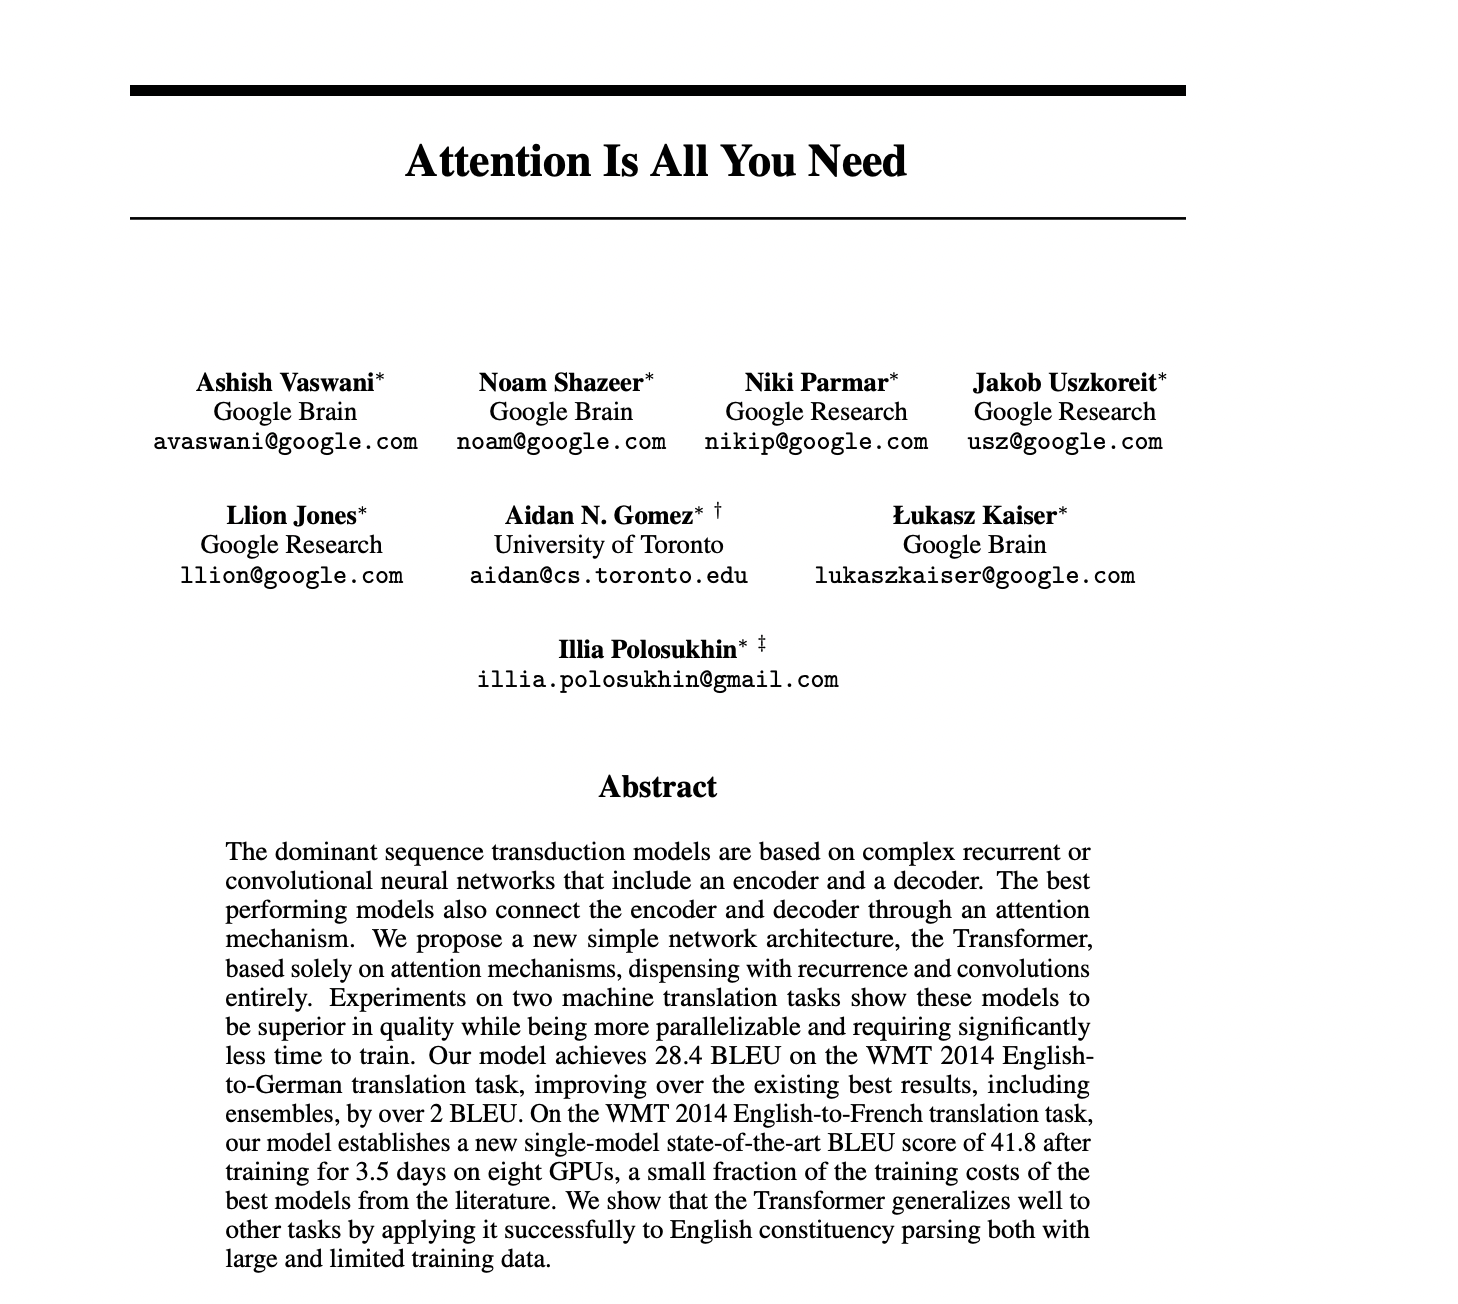
\includegraphics[width=.5\linewidth]{att.png}
	\end{center}
	\vfill
	\footnotesize
	{\color{blue} \url{https://arxiv.org/abs/1706.03762}}
\end{frame}


\begin{frame}{Transformer} 
	\alert{Верхнеуровнего - это просто энкодер и декодер}
	
	\begin{center}
		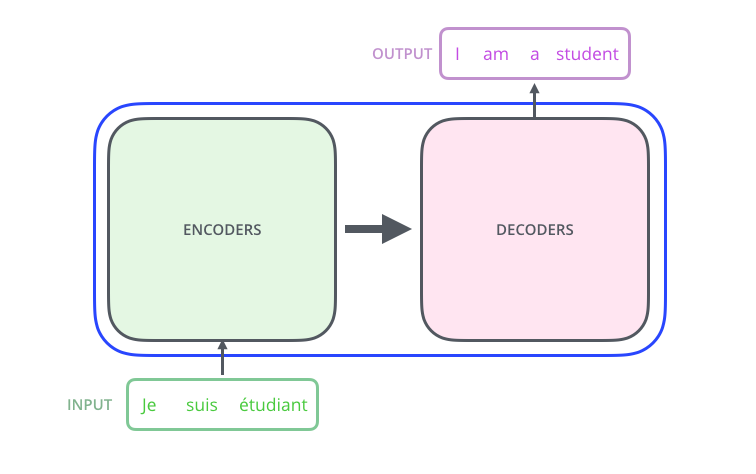
\includegraphics[width=.6\linewidth]{transformer01.png}
	\end{center}
	\vfill
	\footnotesize
	{\color{blue} \url{http://jalammar.github.io/illustrated-transformer/}}
\end{frame}


\begin{frame}{Transformer} 
	Энкодер и декодер состоят из одинаковых блоков; веса во всех блоках разные
	
	\begin{center}
		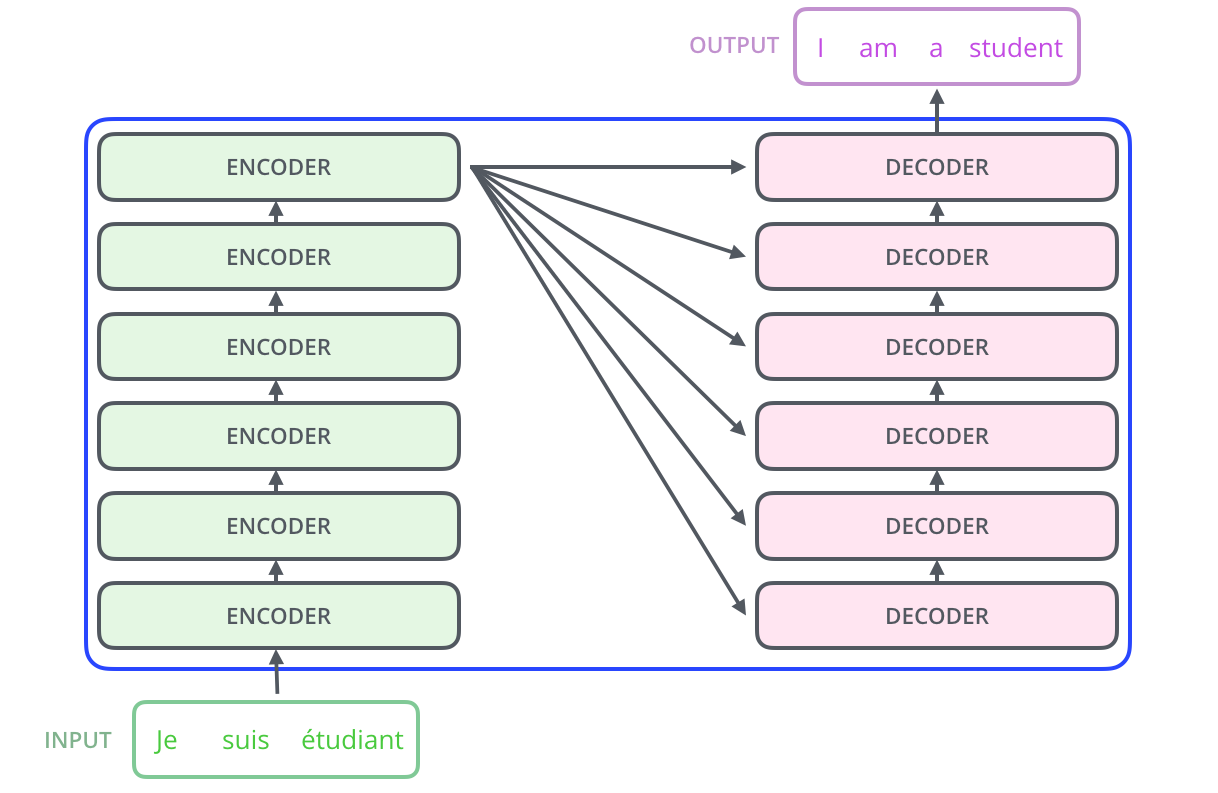
\includegraphics[width=.6\linewidth]{transformer02.png}
	\end{center}
	\vfill
	\footnotesize
	{\color{blue} \url{http://jalammar.github.io/illustrated-transformer/}}
\end{frame}


\begin{frame}{Transformer} 
	В энкодере происходят две вещи: сначала вход прогоняется через self-attention, а затем —
	через полносвязный слой. В декодере помимо обычного self-attention есть ещё и attention
	из энкодера.
	
	\begin{center}
		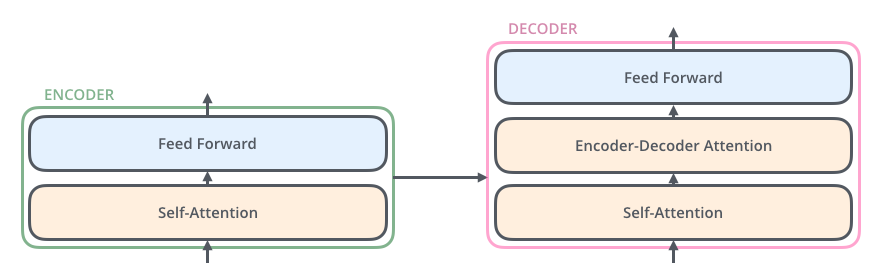
\includegraphics[width=.8\linewidth]{tranformer03.png}
	\end{center}
	\vfill
	\footnotesize
	{\color{blue} \url{http://jalammar.github.io/illustrated-transformer/}}
\end{frame}


\begin{frame}{Self-attention} 
	\begin{center}
		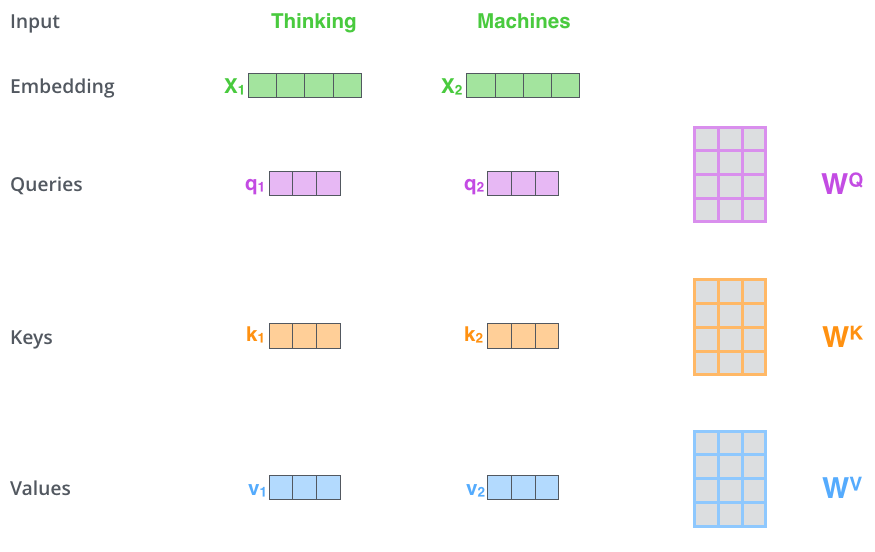
\includegraphics[width=.7\linewidth]{selfattention.png}
	\end{center}
\end{frame}


\begin{frame}{Абстракции}
	\begin{wideitemize}
		\item  Для каждого входного слова считаются три вектора: Query, Key и Value
		\item  Матрицы $W^Q, W^K , W^V$ обучаются вместе с моделью
		\item  Value - то, что мы знаем об этом слове
		\item  Query, Key помогают искать связи между словами, мы ходим по всем словам и пытаемся понять насколько они связаны между собой 
		\item Query - мое текущее слово, Key - мое слово с которым я сравниваю себя
	\end{wideitemize}
\end{frame}


\begin{frame}{Self-attention} 
	Цель этого слоя — сложить Value с некоторыми весами
	
	\begin{center}
		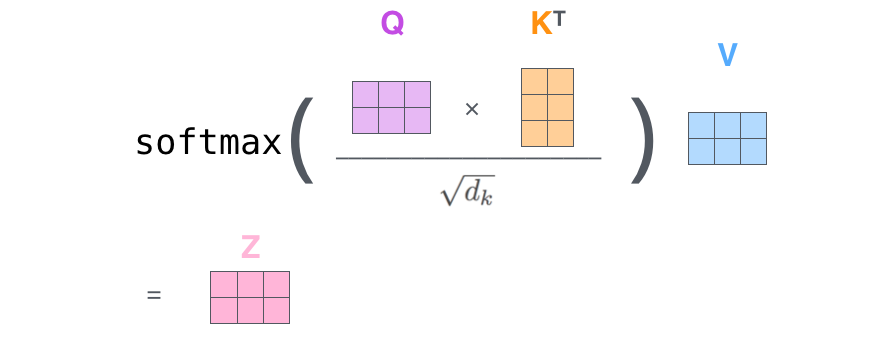
\includegraphics[width=.9\linewidth]{self_final.png}
	\end{center}
\end{frame}


\begin{frame}{Более детально}
	\centering
	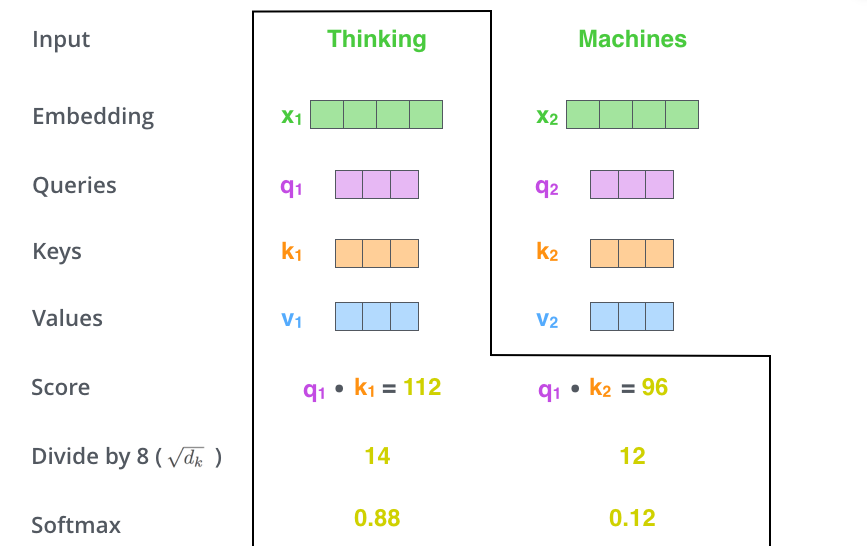
\includegraphics[width=0.8\linewidth]{step_3}
\end{frame}


\begin{frame}{Более детально}
	\centering
	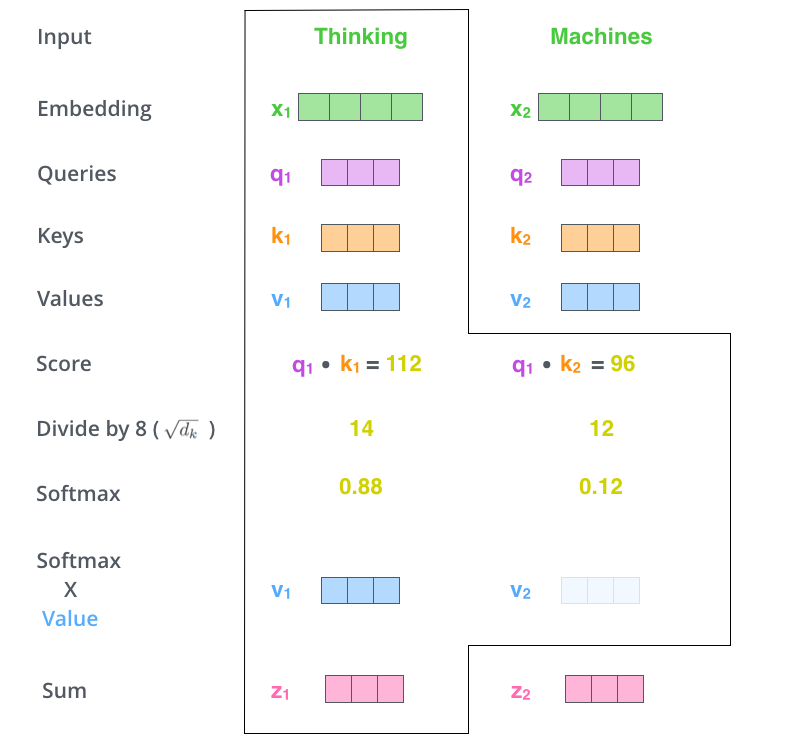
\includegraphics[width=0.5\linewidth]{step_4}
\end{frame}


\begin{frame}{Query, Key, Value}
	\begin{center}
	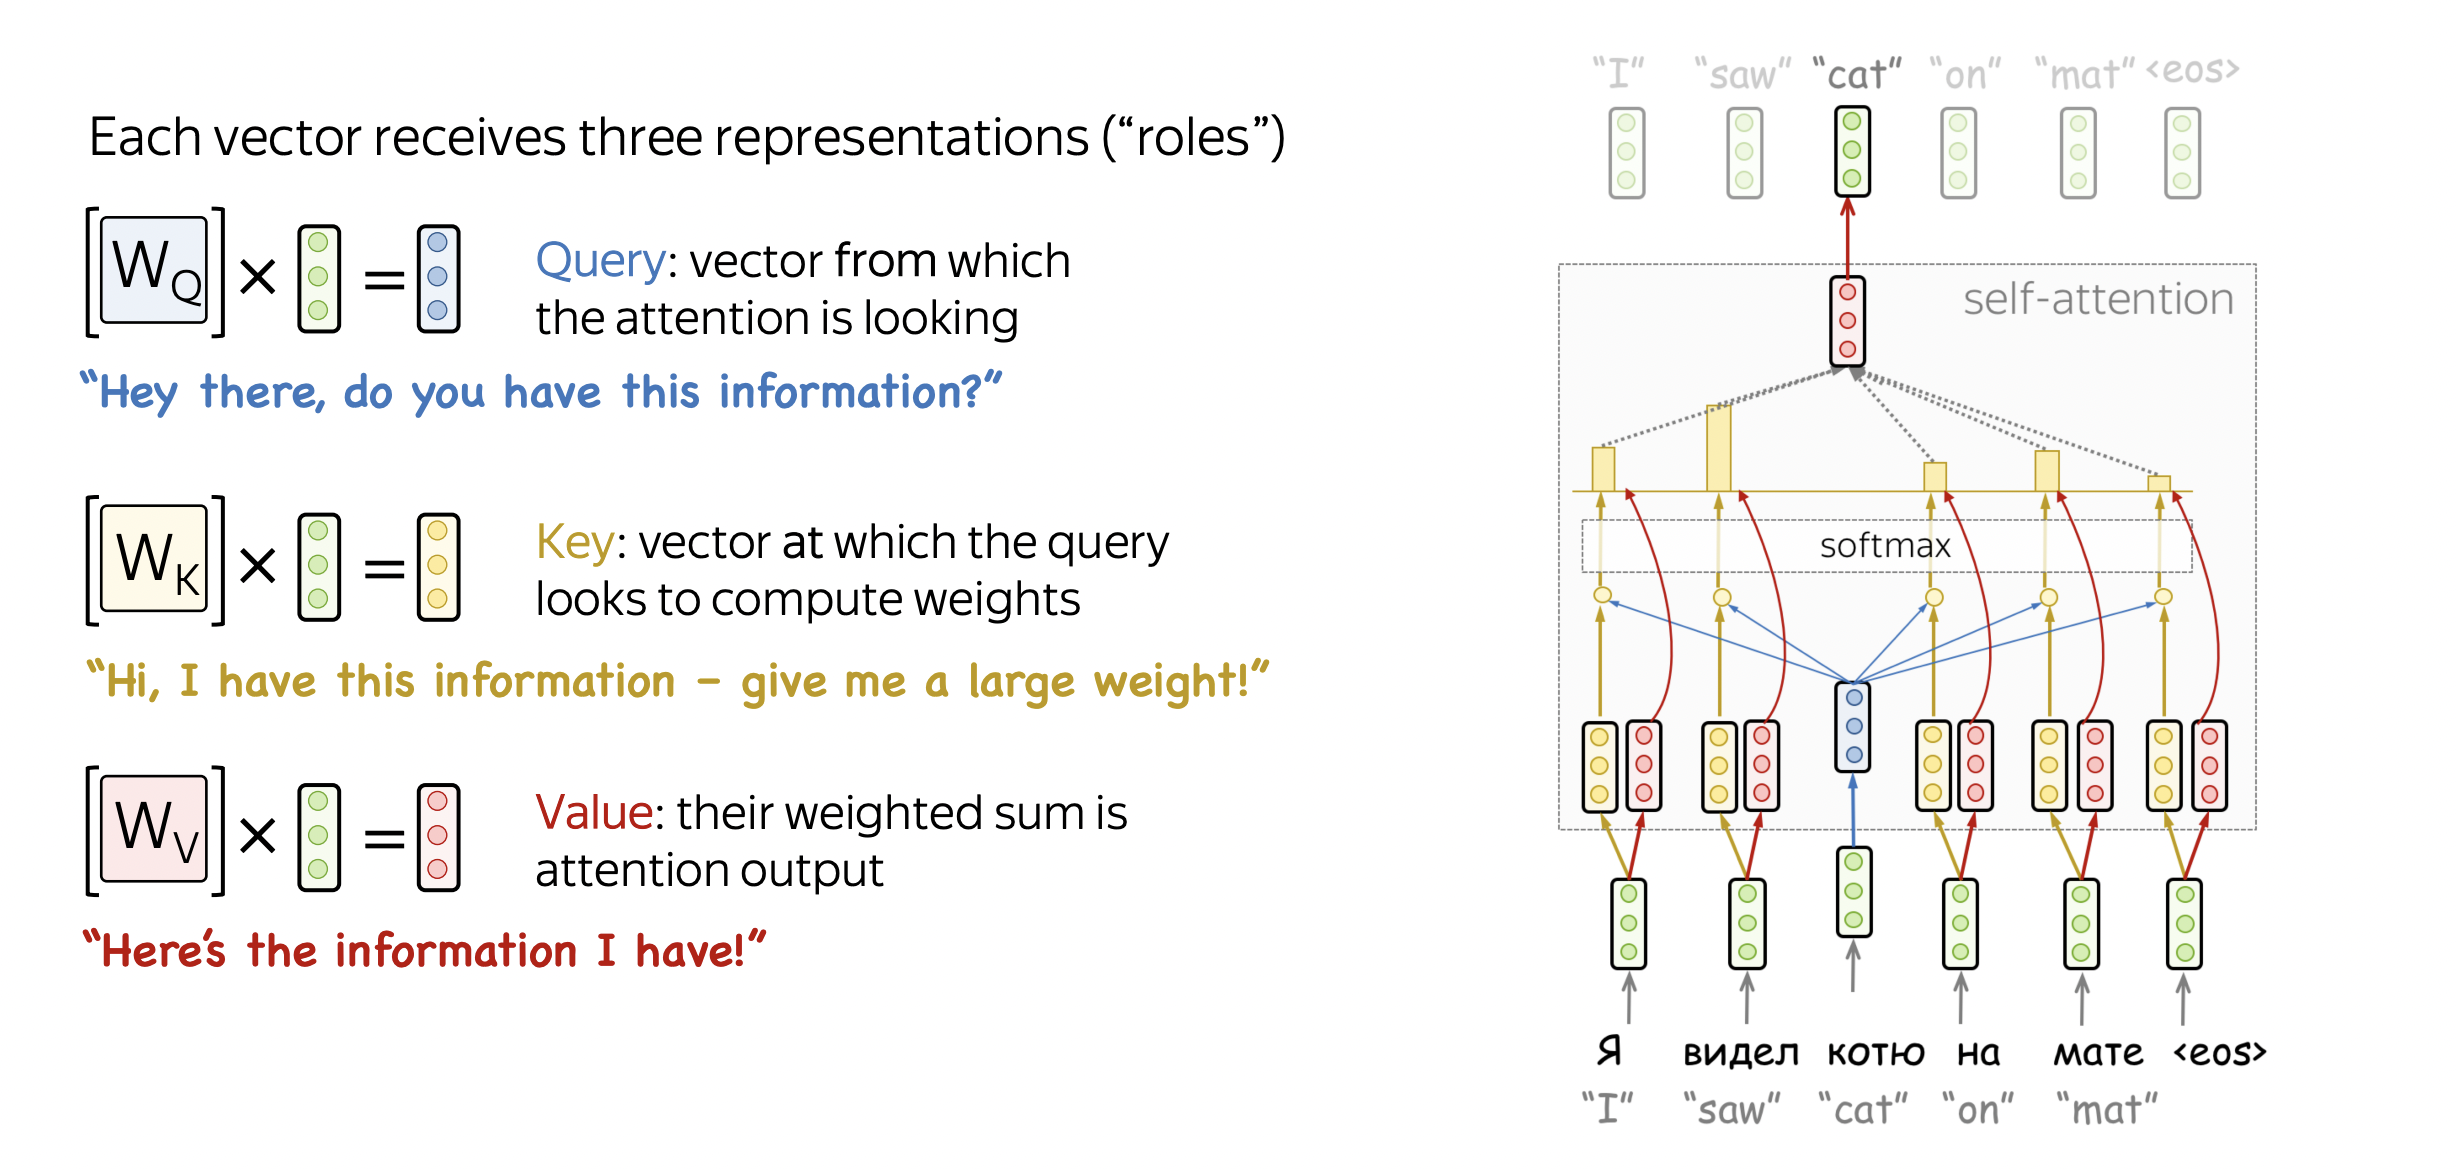
\includegraphics[width=.95\linewidth]{qkv1.png}
	\end{center}
	\vfill
	\footnotesize  {\color{blue} \url{https://github.com/yandexdataschool/nlp_course/tree/2021/week04_seq2seq}} 
\end{frame}


\begin{frame}{Query, Key, Value}
	\begin{center}
		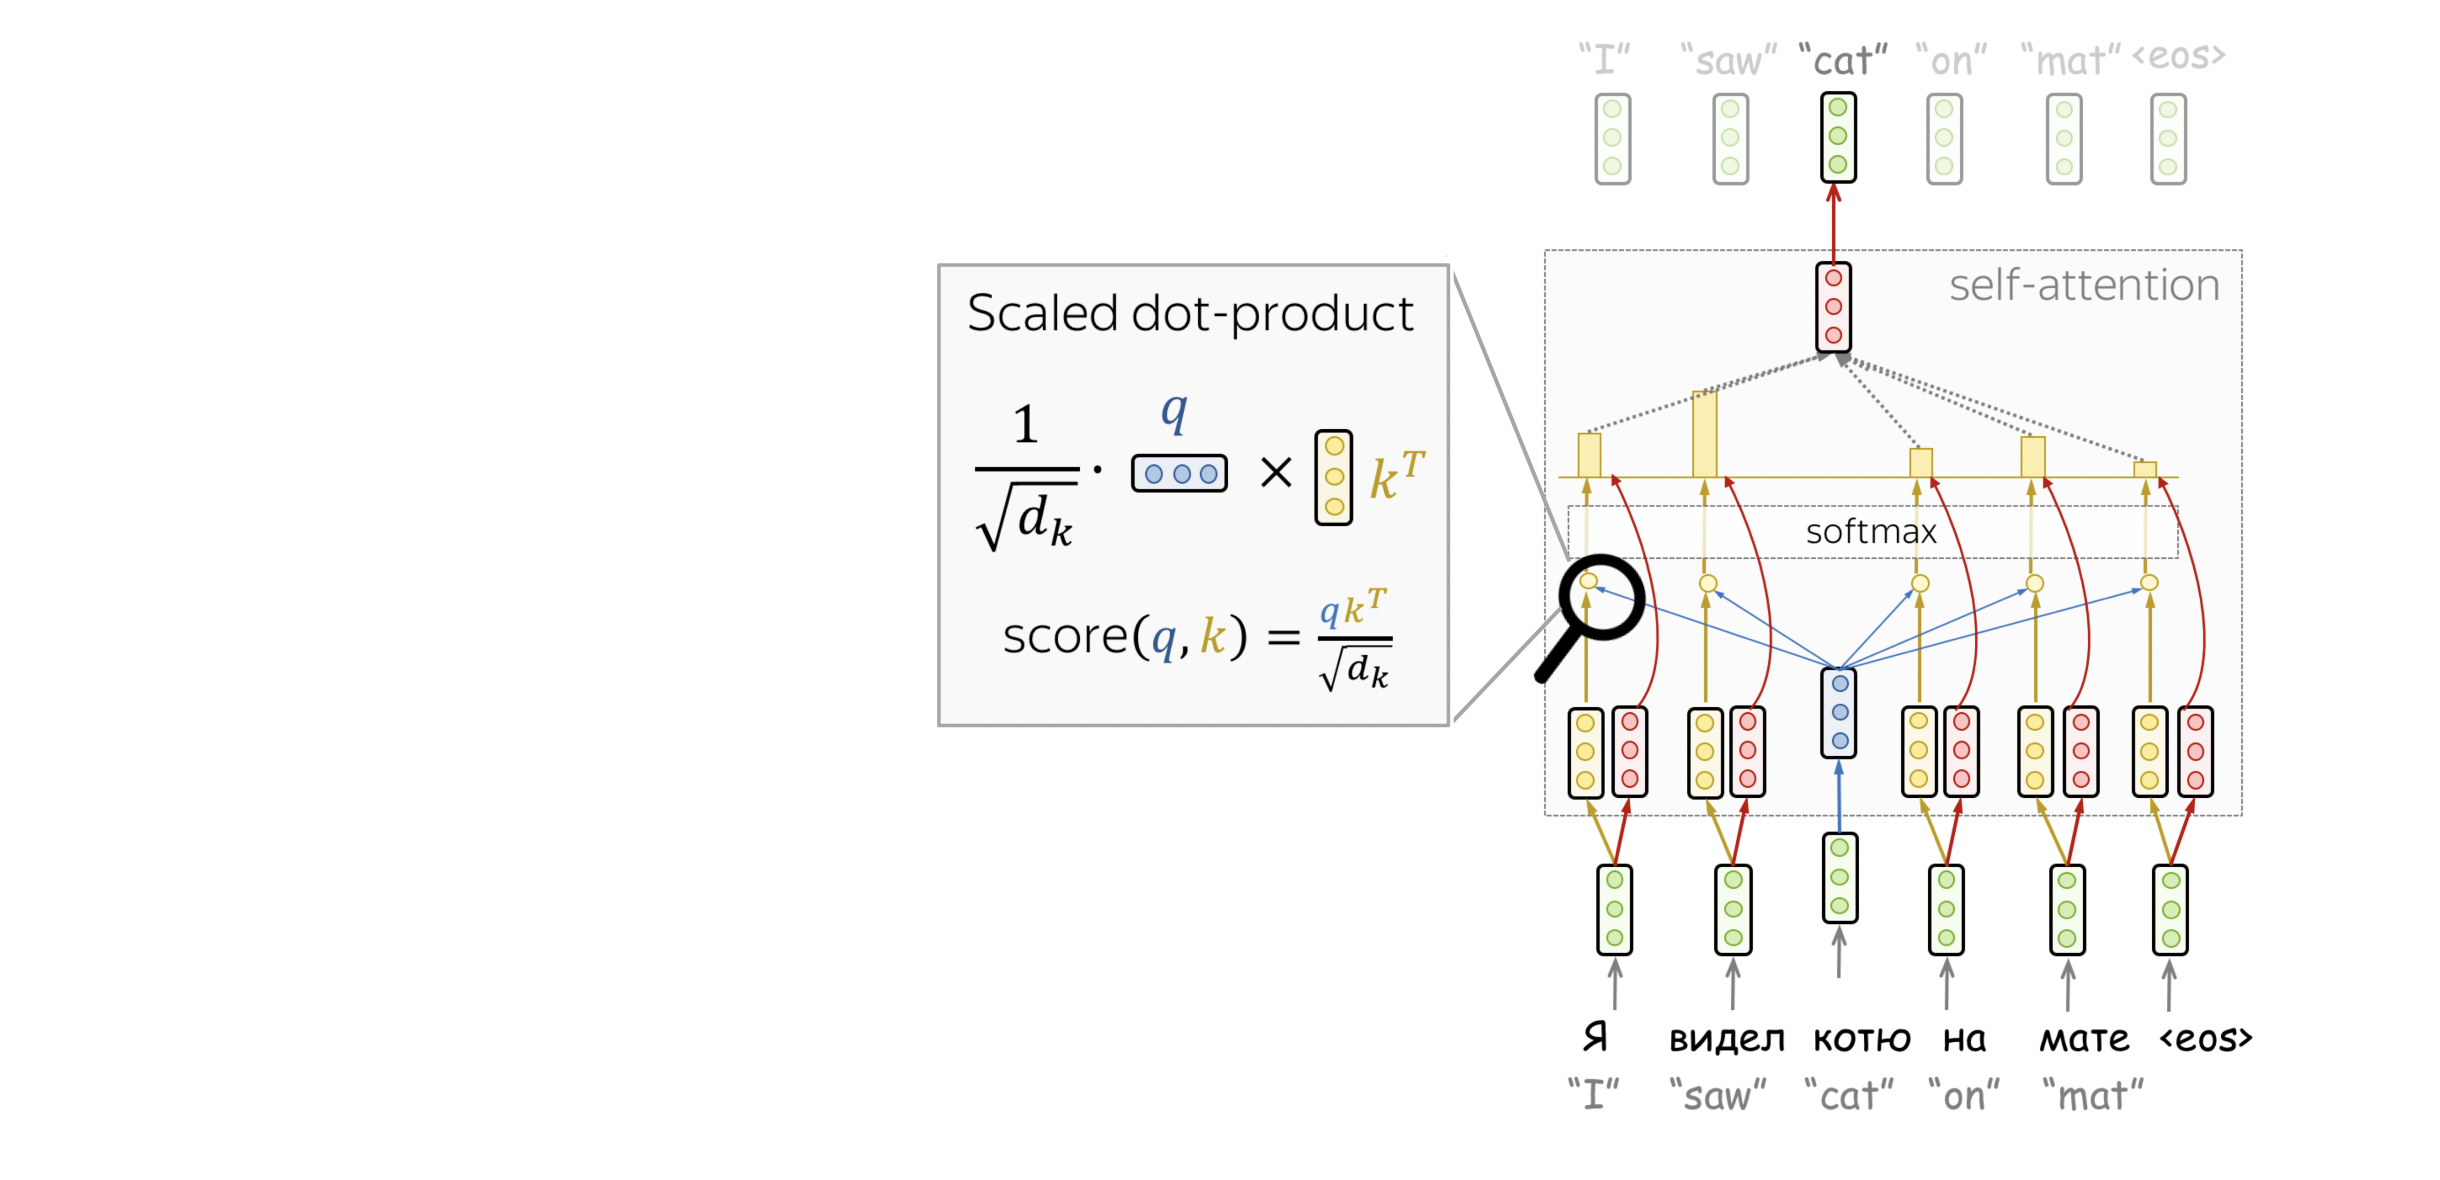
\includegraphics[width=.95\linewidth]{qkv2.png}
	\end{center}
	\vfill
	\footnotesize  {\color{blue} \url{https://github.com/yandexdataschool/nlp_course/tree/2021/week04_seq2seq}} 
\end{frame}


\begin{frame}{Query, Key, Value}
	\begin{center}
		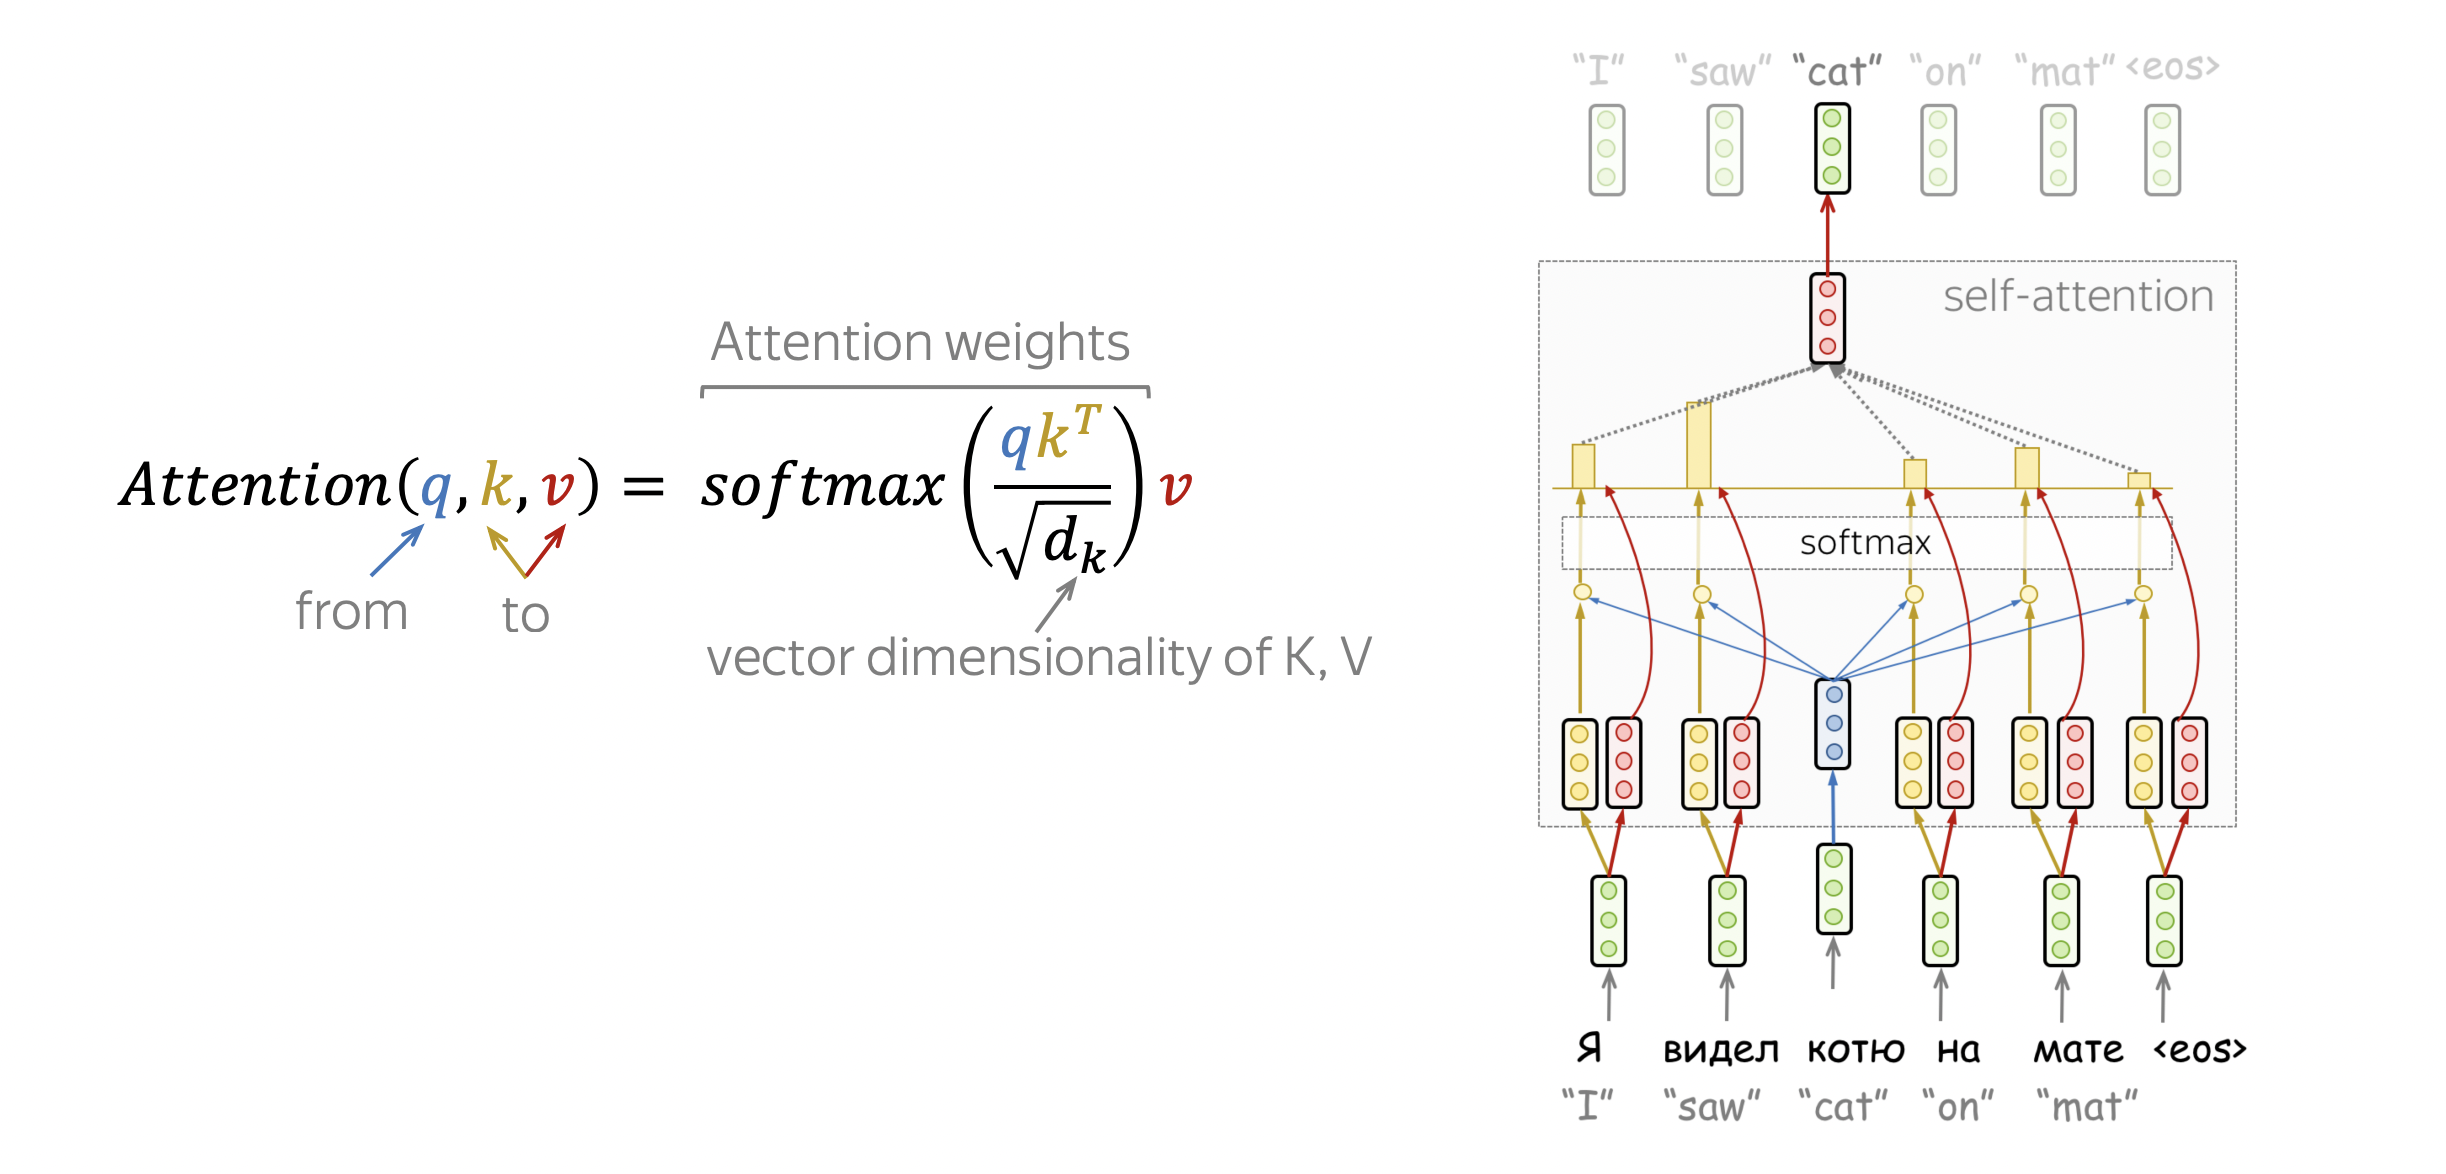
\includegraphics[width=.95\linewidth]{qkv3.png}
	\end{center}
	\vfill
	\footnotesize  {\color{blue} \url{https://github.com/yandexdataschool/nlp_course/tree/2021/week04_seq2seq}} 
\end{frame}


\begin{frame}{Masked Self-Attention}
	\begin{center}
		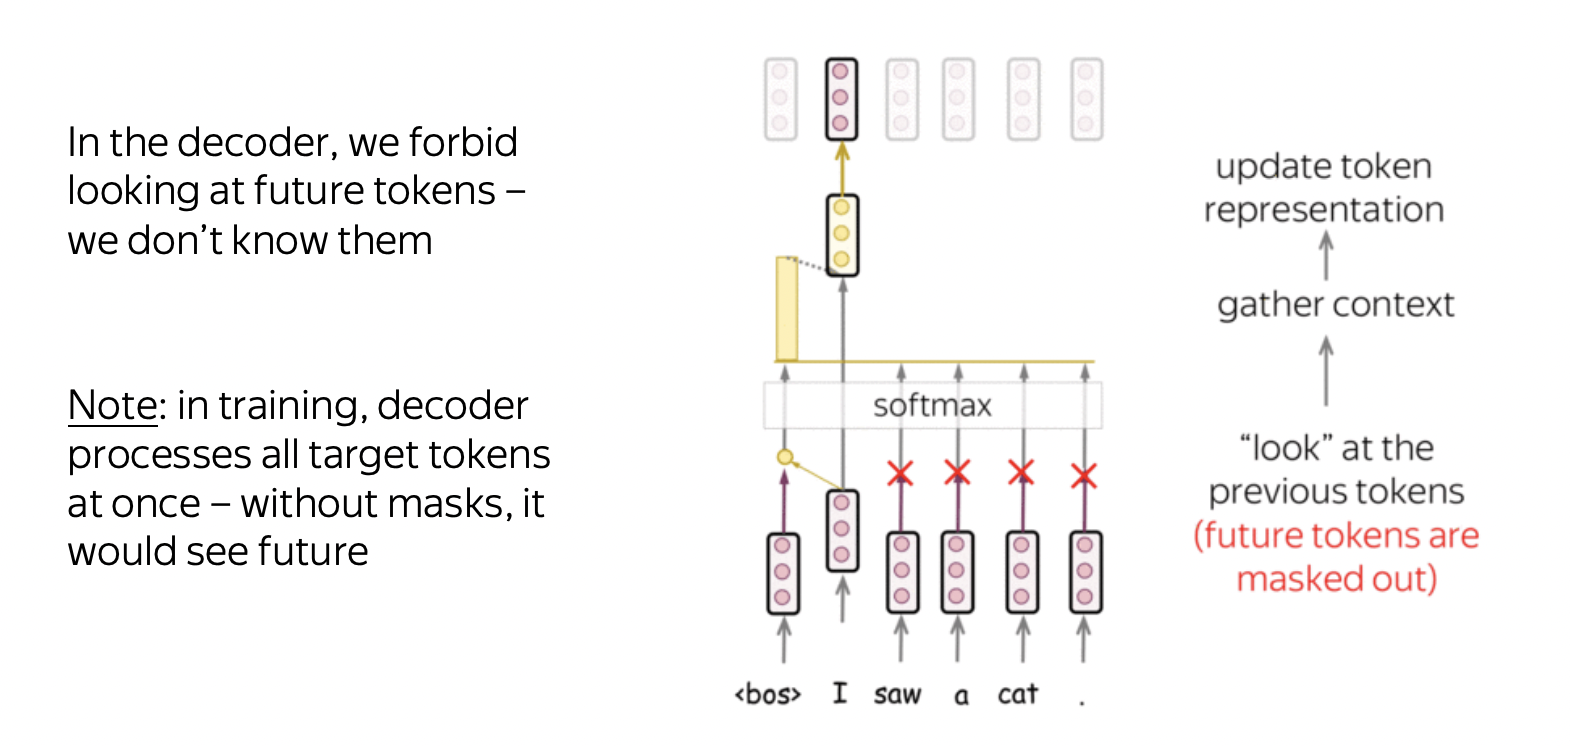
\includegraphics[width=.95\linewidth]{qkv4.png}
	\end{center}
	\vfill
	\footnotesize  {\color{blue} \url{https://github.com/yandexdataschool/nlp_course/tree/2021/week04_seq2seq}} 
\end{frame}


\begin{transitionframe}
	\begin{center}
		\Huge Зверь с кучей голов
	\end{center}
\end{transitionframe}


\begin{frame}{Зверь с кучей голов} 
		Несколько голов обеспечивают разное внимание
		\begin{center}
			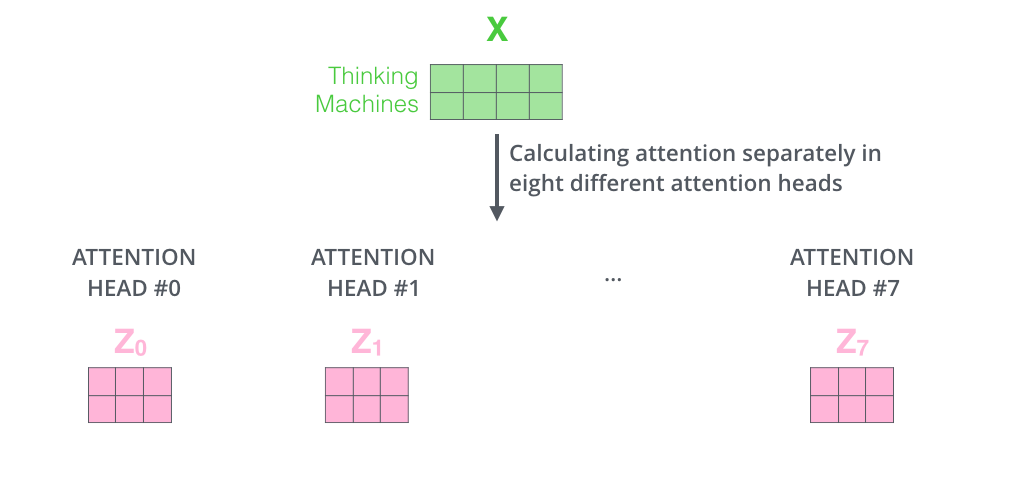
\includegraphics[width=.8\linewidth]{many_hads.png}
		\end{center}
\end{frame}


\begin{frame}{Слой целиком} 
		\begin{center}
			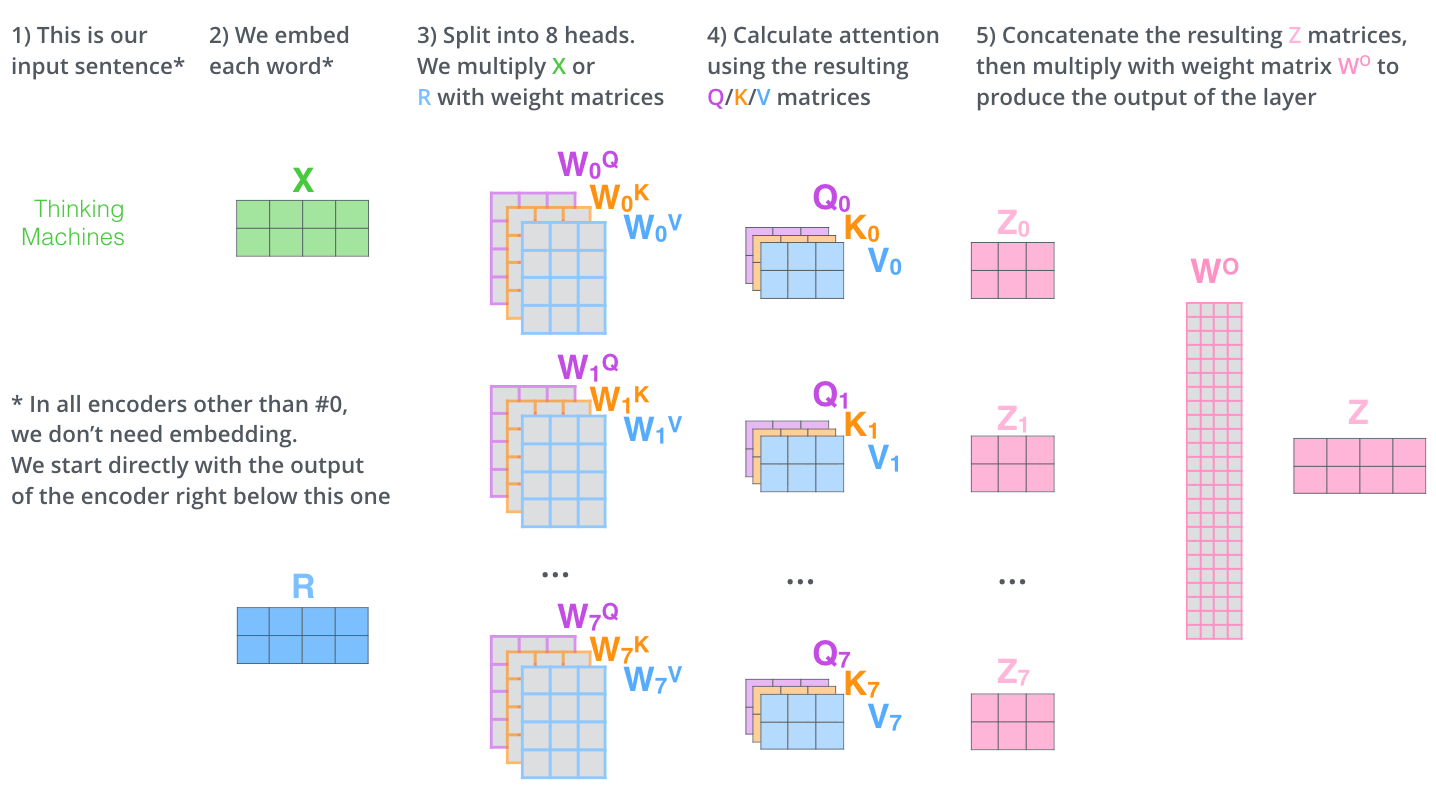
\includegraphics[width=.85\linewidth]{together.png}
		\end{center}
\end{frame}


\begin{frame}{Multi-Head Attention} 
	\begin{center}
		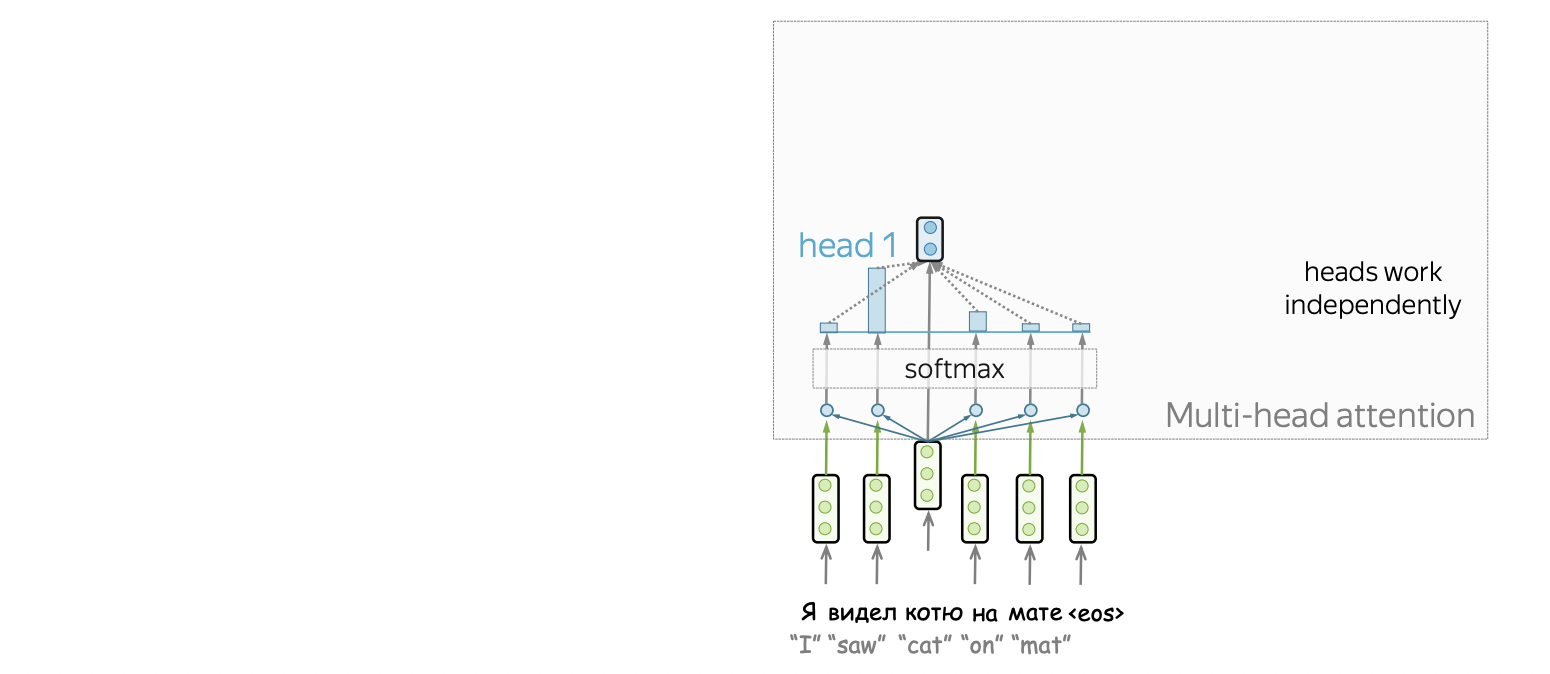
\includegraphics[width=.99\linewidth]{mh1.png}
	\end{center}
	\vfill
\footnotesize  {\color{blue} \url{https://github.com/yandexdataschool/nlp_course/tree/2021/week04_seq2seq}} 
\end{frame}


\begin{frame}{Multi-Head Attention} 
	\begin{center}
		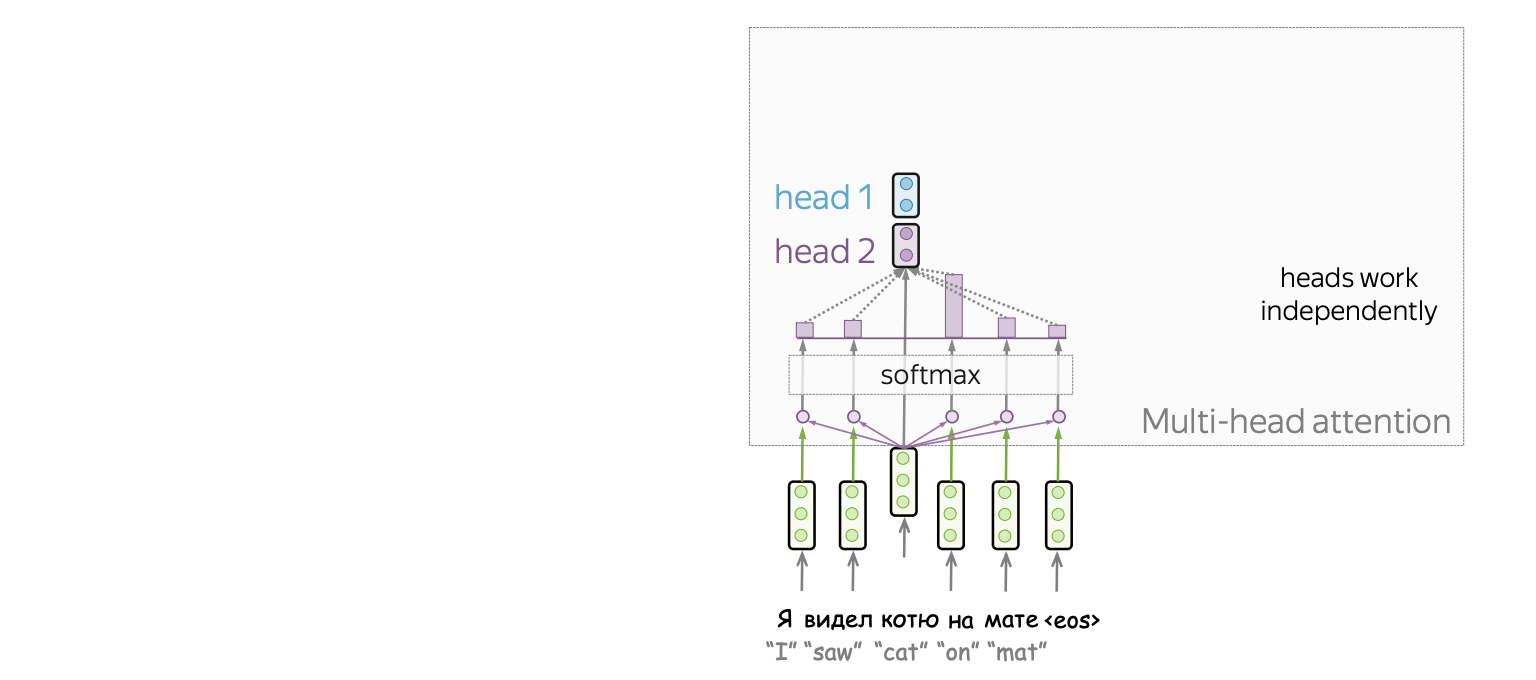
\includegraphics[width=.99\linewidth]{mh2.png}
	\end{center}
	\vfill
\footnotesize  {\color{blue} \url{https://github.com/yandexdataschool/nlp_course/tree/2021/week04_seq2seq}} 
\end{frame}


\begin{frame}{Multi-Head Attention} 
	\begin{center}
		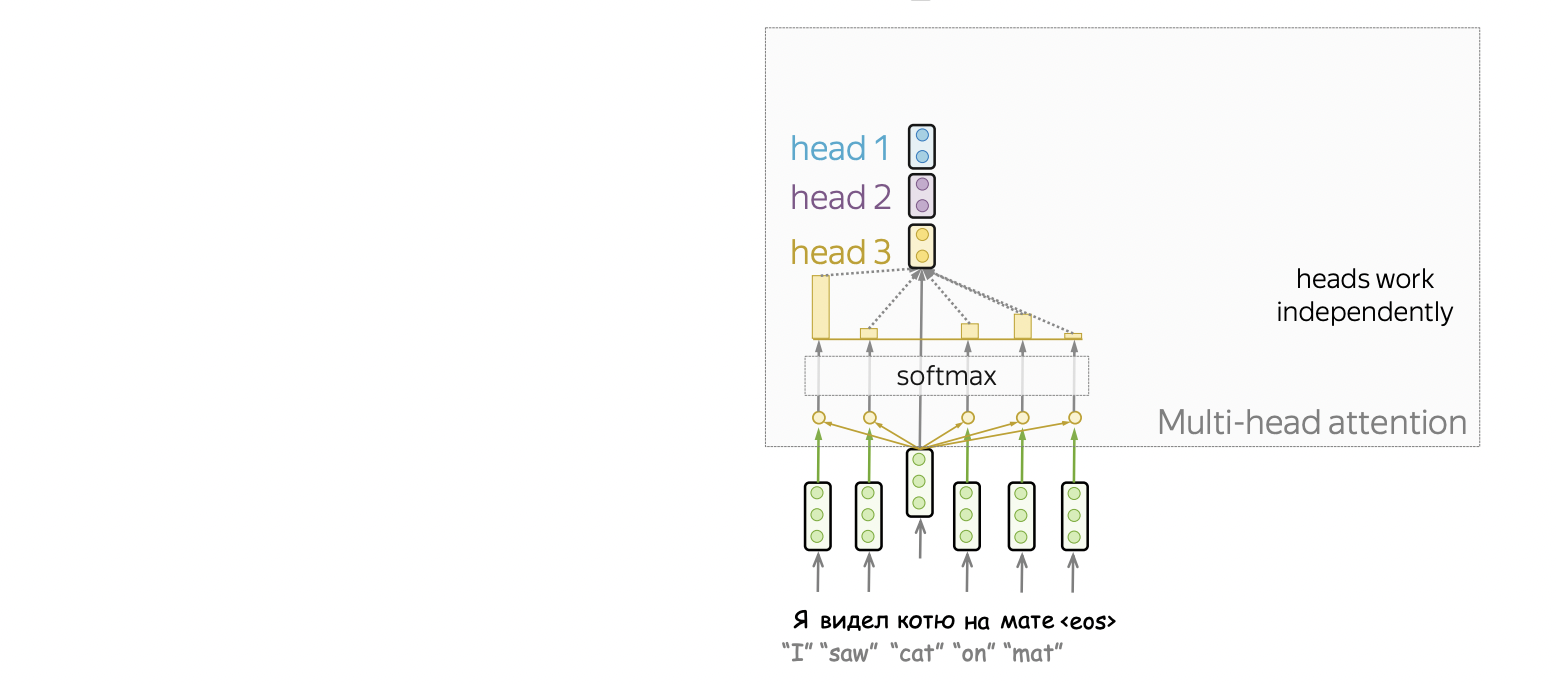
\includegraphics[width=.99\linewidth]{mh3.png}
	\end{center}
	\vfill
\footnotesize  {\color{blue} \url{https://github.com/yandexdataschool/nlp_course/tree/2021/week04_seq2seq}} 
\end{frame}


\begin{frame}{Multi-Head Attention} 
	\begin{center}
		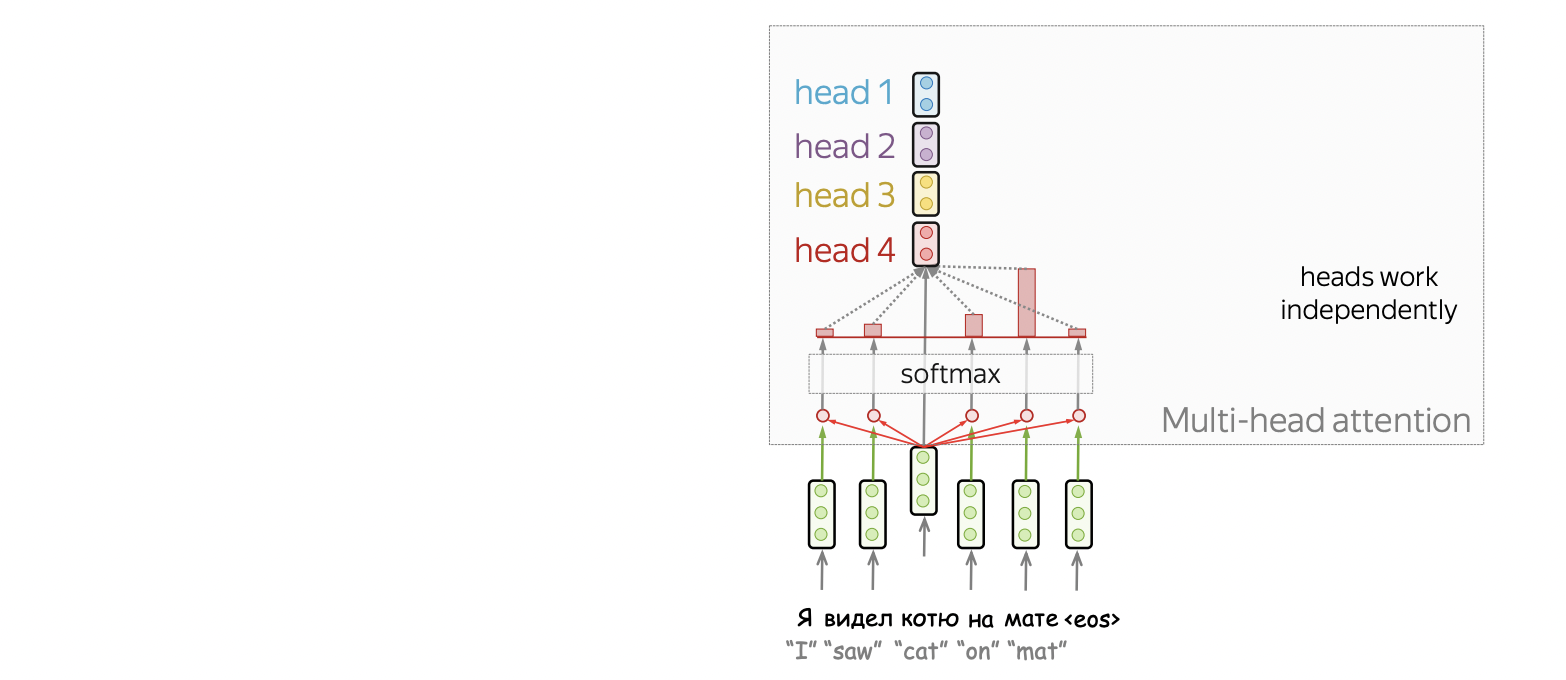
\includegraphics[width=.99\linewidth]{mh4.png}
	\end{center}
	\vfill
\footnotesize  {\color{blue} \url{https://github.com/yandexdataschool/nlp_course/tree/2021/week04_seq2seq}} 
\end{frame}


\begin{frame}{Multi-Head Attention} 
	\begin{center}
		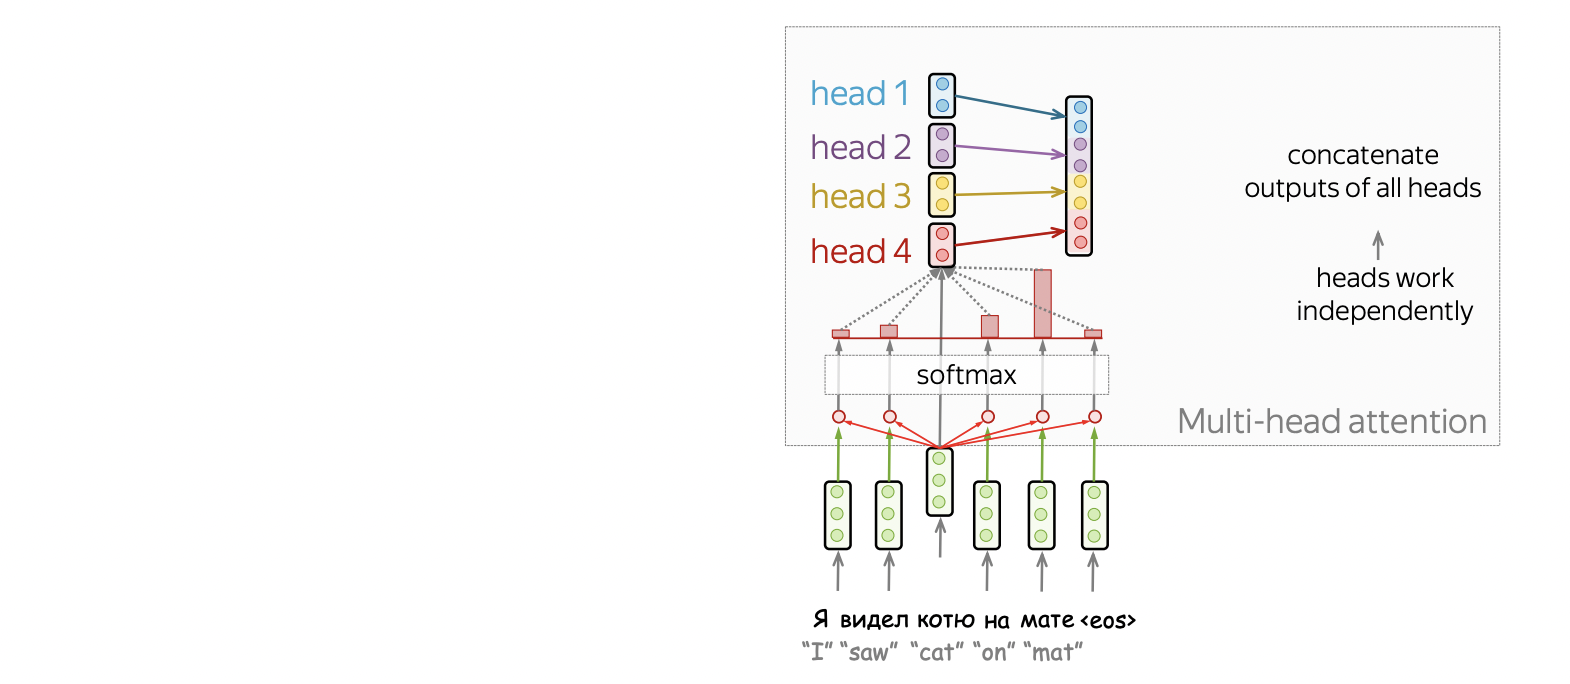
\includegraphics[width=.99\linewidth]{mh5.png}
	\end{center}
	\vfill
\footnotesize  {\color{blue} \url{https://github.com/yandexdataschool/nlp_course/tree/2021/week04_seq2seq}} 
\end{frame}


\begin{frame}{Multi-Head Attention} 
	\begin{center}
		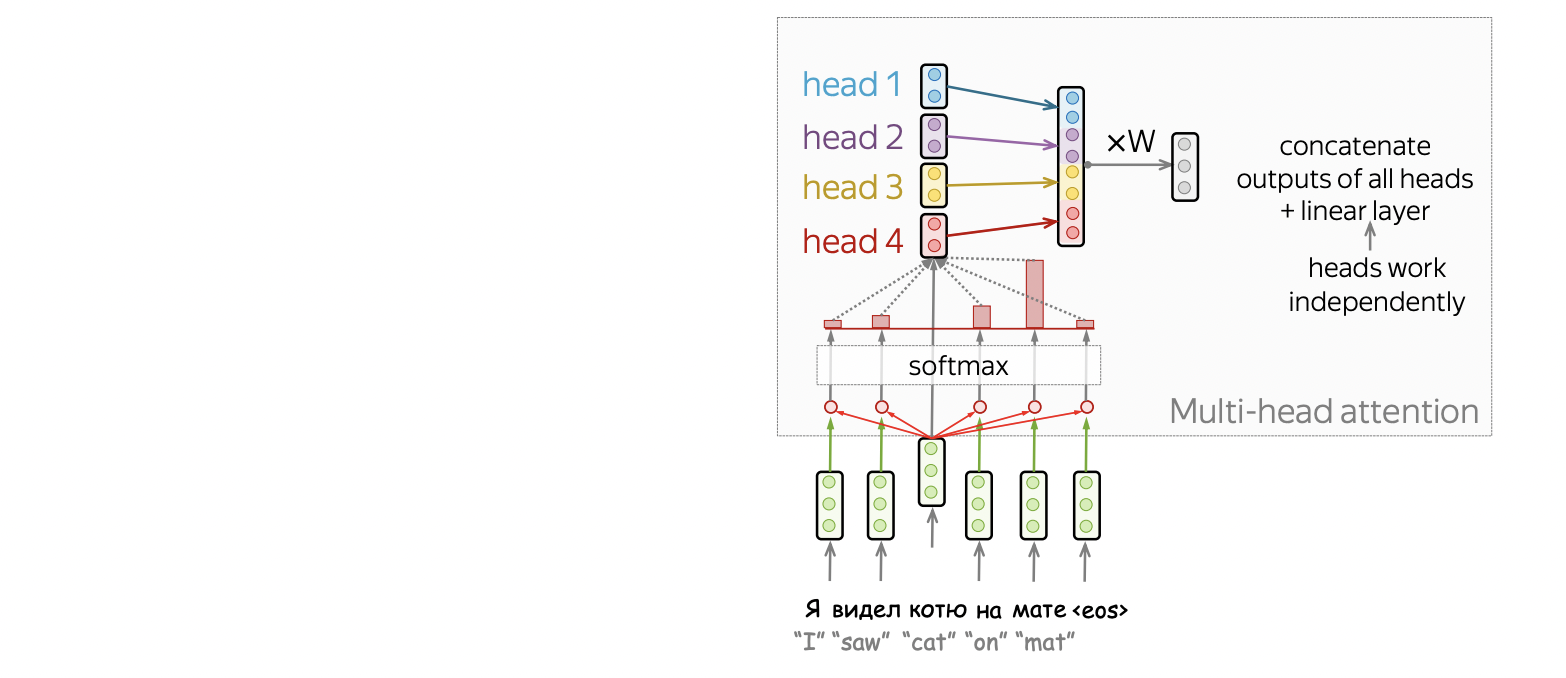
\includegraphics[width=.99\linewidth]{mh6.png}
	\end{center}
	\vfill
\footnotesize  {\color{blue} \url{https://github.com/yandexdataschool/nlp_course/tree/2021/week04_seq2seq}} 
\end{frame}


\begin{frame}{Multi-Head Attention} 
	\begin{center}
		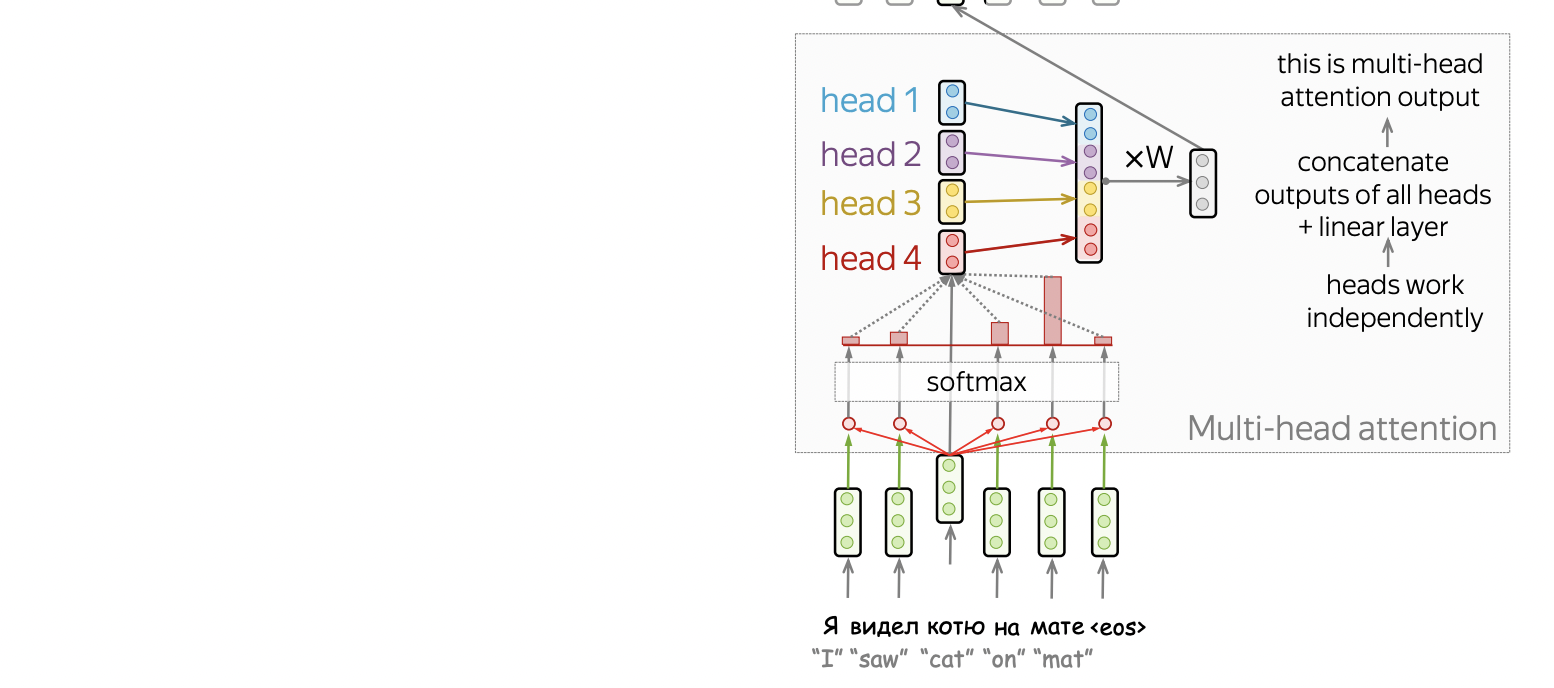
\includegraphics[width=.99\linewidth]{mh7.png}
	\end{center}
	\vfill
\footnotesize  {\color{blue} \url{https://github.com/yandexdataschool/nlp_course/tree/2021/week04_seq2seq}} 
\end{frame}


\begin{transitionframe}
	\begin{center}
		\Huge Positional Encoding
	\end{center}
\end{transitionframe}


\begin{frame}{Positional encoding} 
		Для учёта позиции можно приплюсовать дополнительный вектор
		
		\begin{center}
			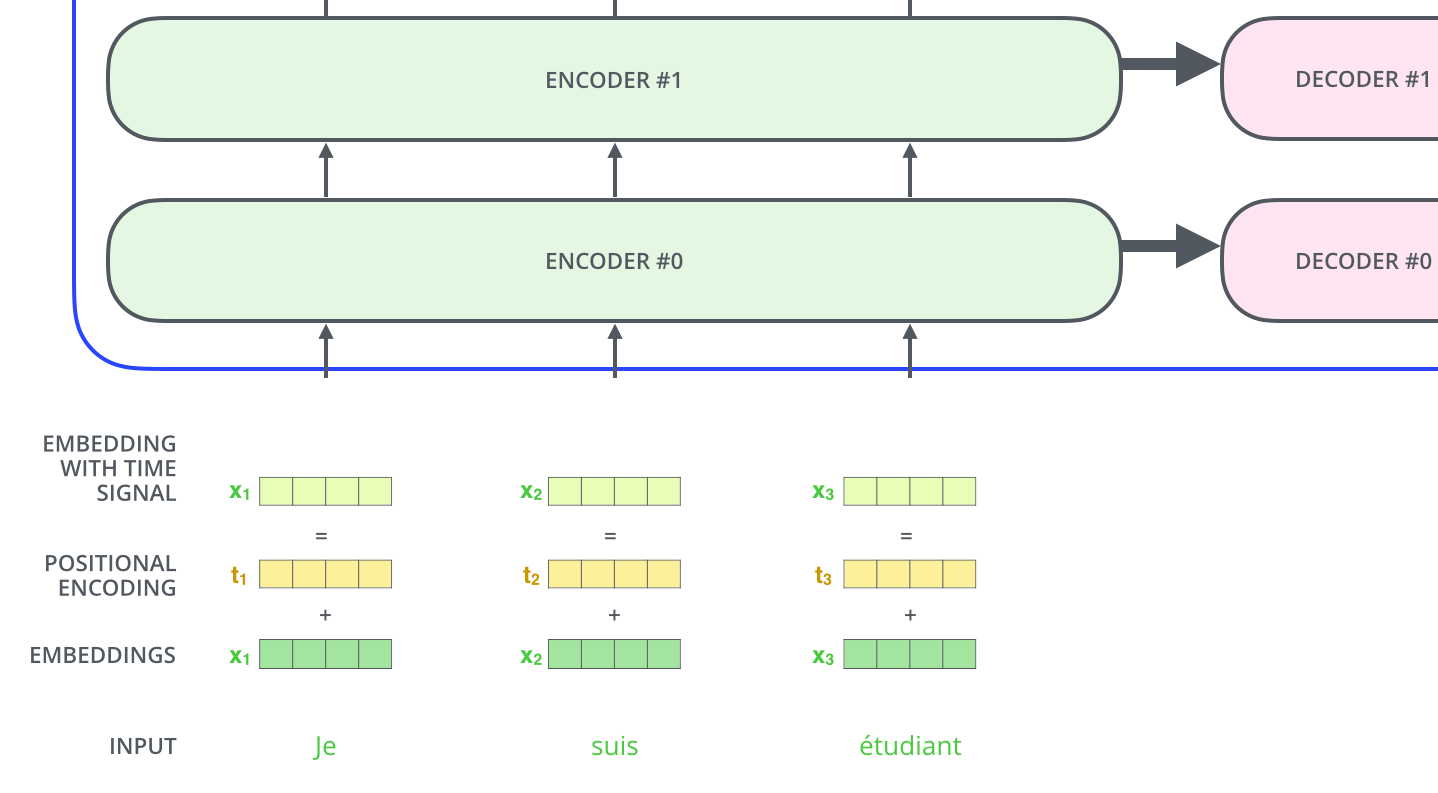
\includegraphics[width=.8\linewidth]{positional_encoding.png}
		\end{center}
\end{frame}


\begin{frame}{Positional encoding} 
	Можно закодировать позицию с помощью синусоиды или какого-нибудь OHE-вектора
	\begin{center}
		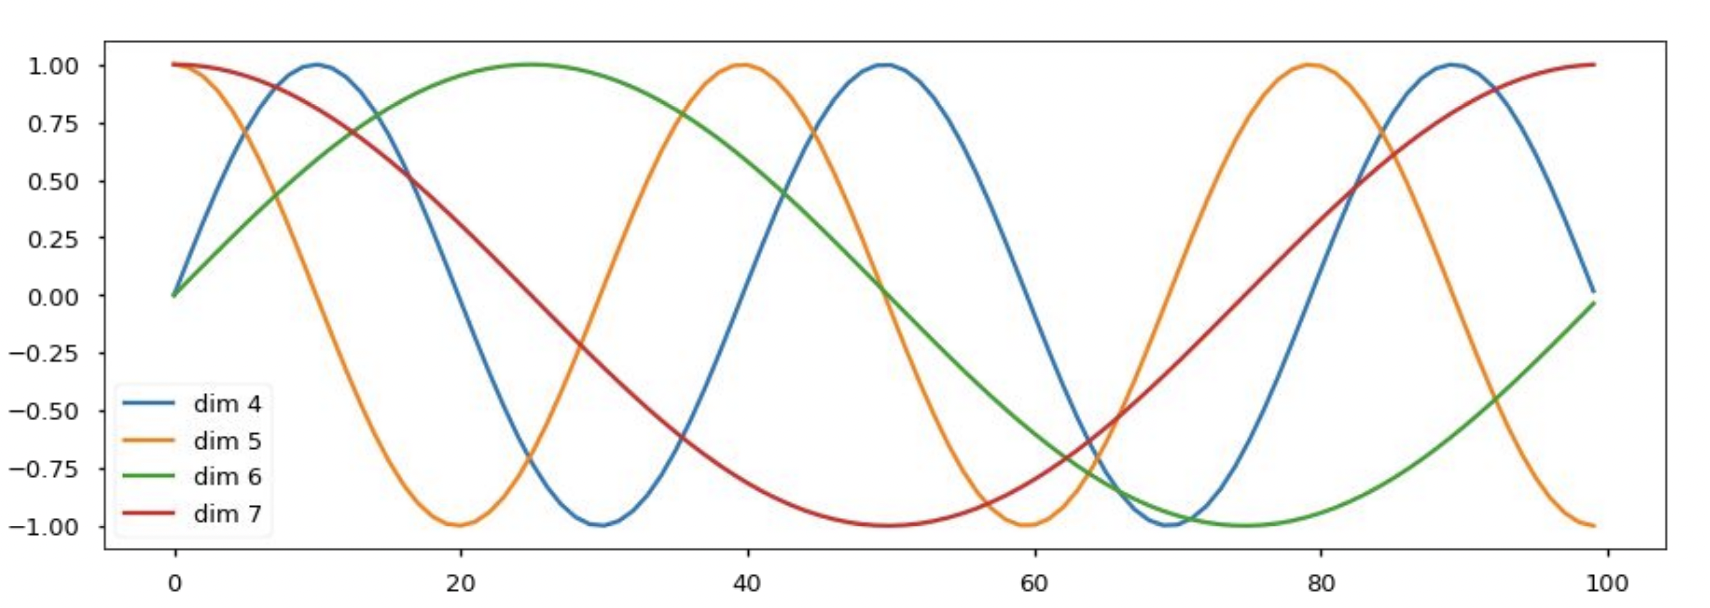
\includegraphics[width=.9\linewidth]{pos2.png}
	\end{center}
\end{frame}


\begin{frame}{Positional encoding} 
	\begin{center}
		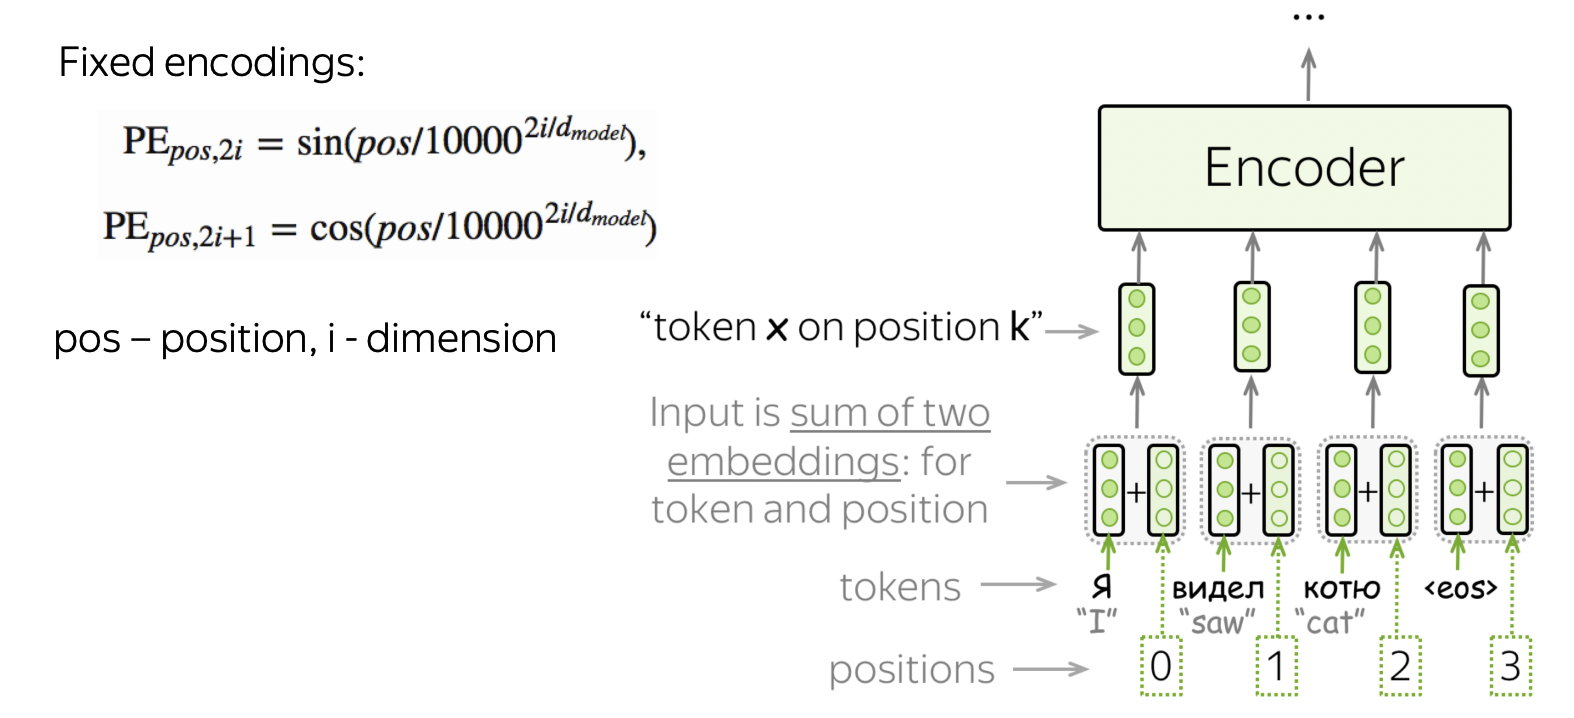
\includegraphics[width=.9\linewidth]{pos3.png}
	\end{center}
\end{frame}


\begin{transitionframe}
	\begin{center}
		\Huge Энкодер и декодер
	\end{center}
\end{transitionframe}


\begin{frame}{Что происходит в энкодере} 
		\begin{center}
			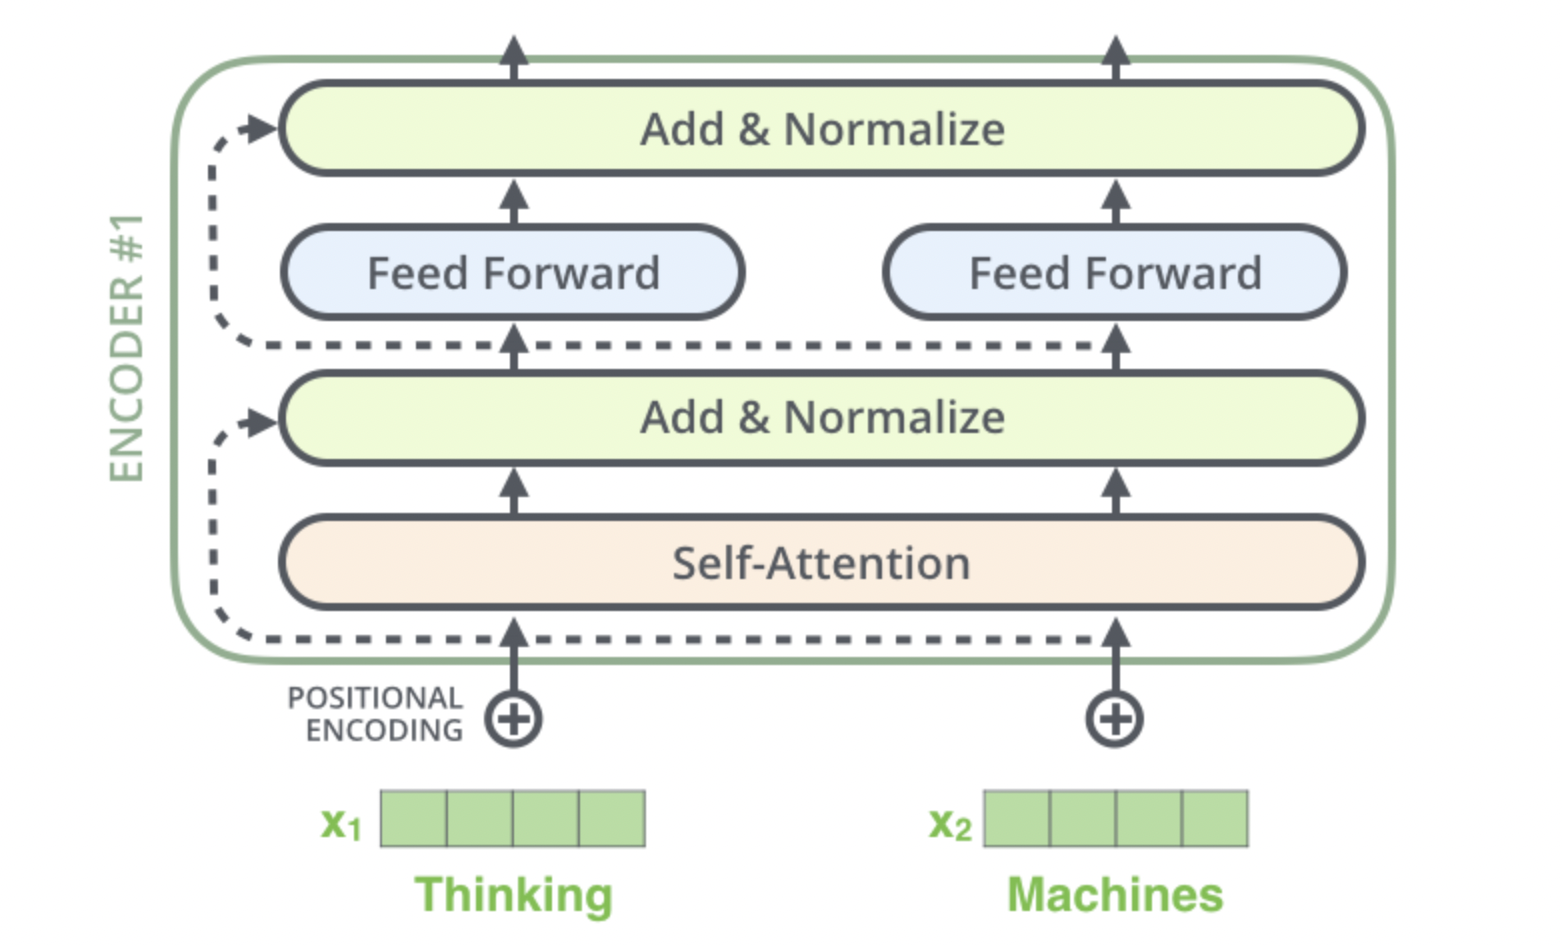
\includegraphics[width=.75\linewidth]{encoder1.png}
		\end{center}
		\vfill
		\footnotesize
		{\color{blue} \url{http://jalammar.github.io/illustrated-transformer/}}
\end{frame}


\begin{frame}{Что происходит в энкодере} 
	\begin{center}
		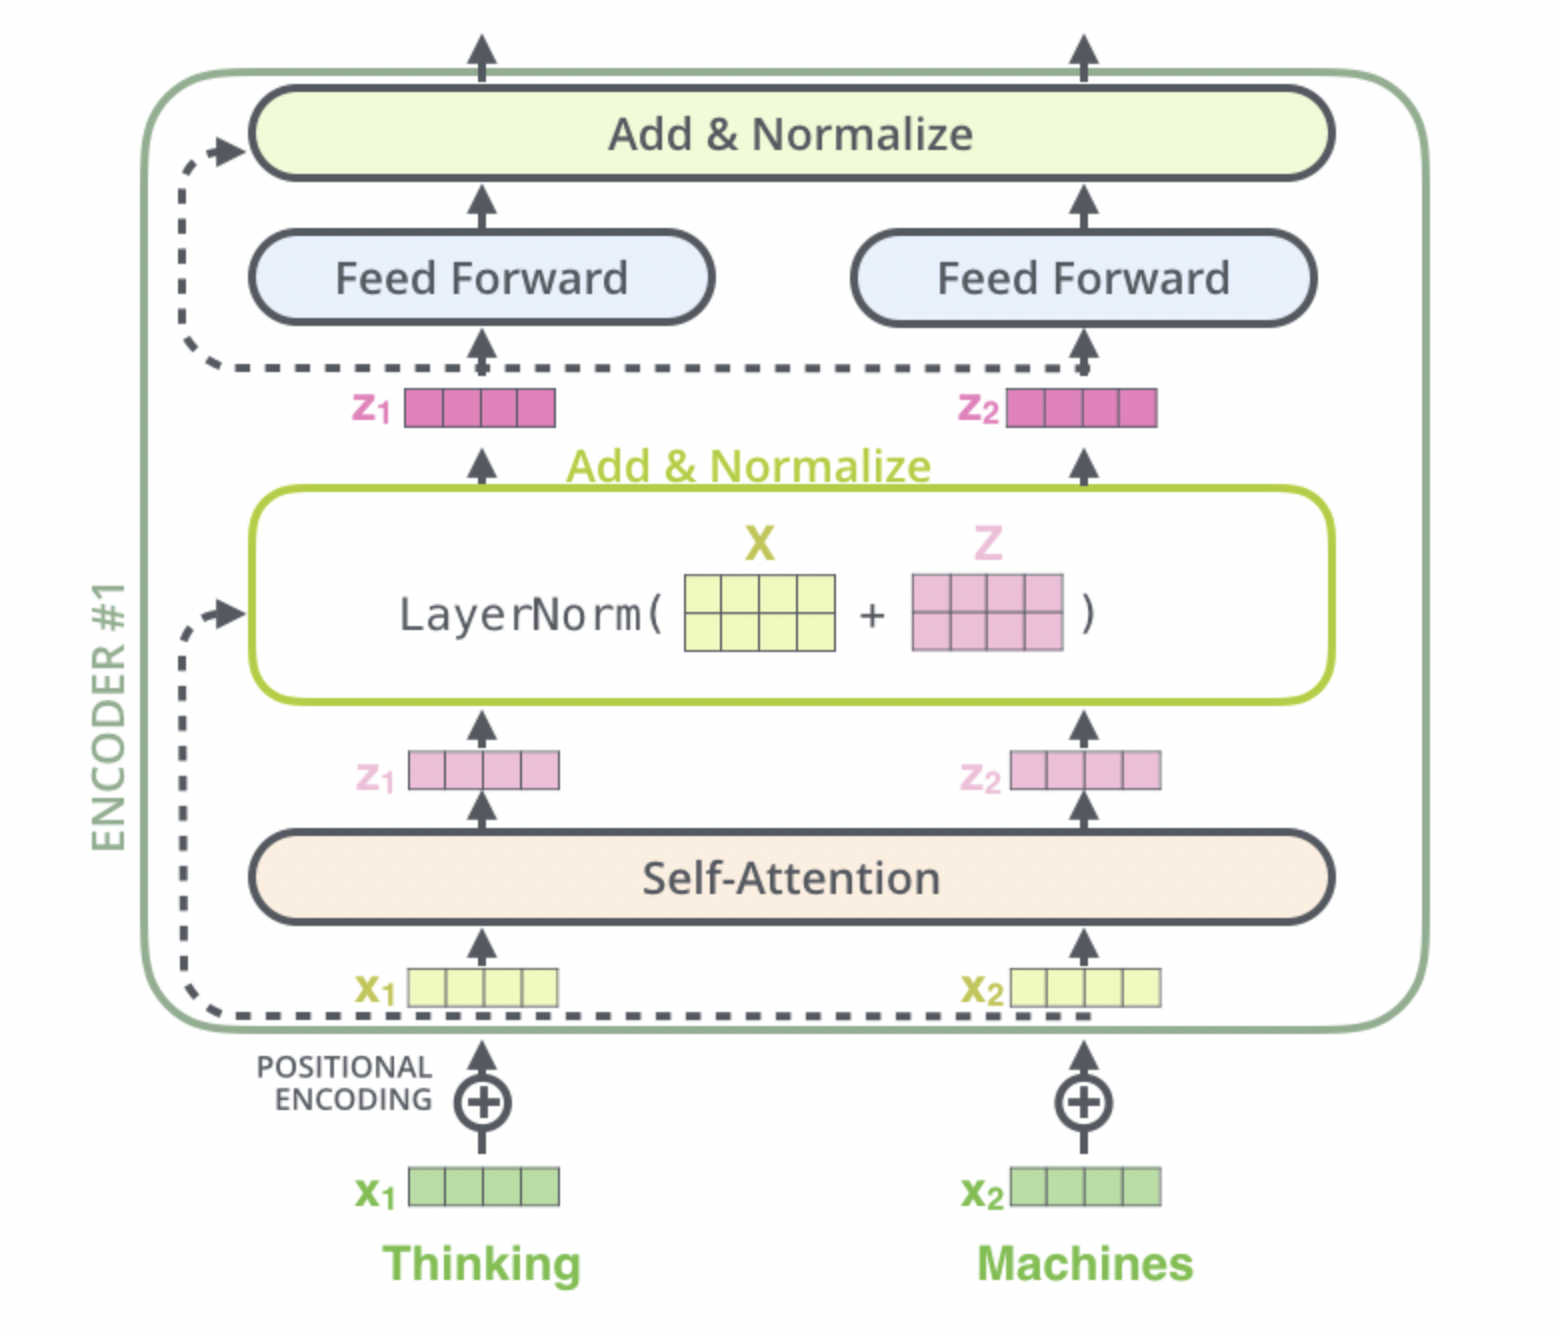
\includegraphics[width=.6\linewidth]{encoder2.png}
	\end{center}
	\vfill
	\footnotesize
	{\color{blue} \url{http://jalammar.github.io/illustrated-transformer/}}
\end{frame}


\begin{frame}{Layer Normalization} 
	\begin{center}
		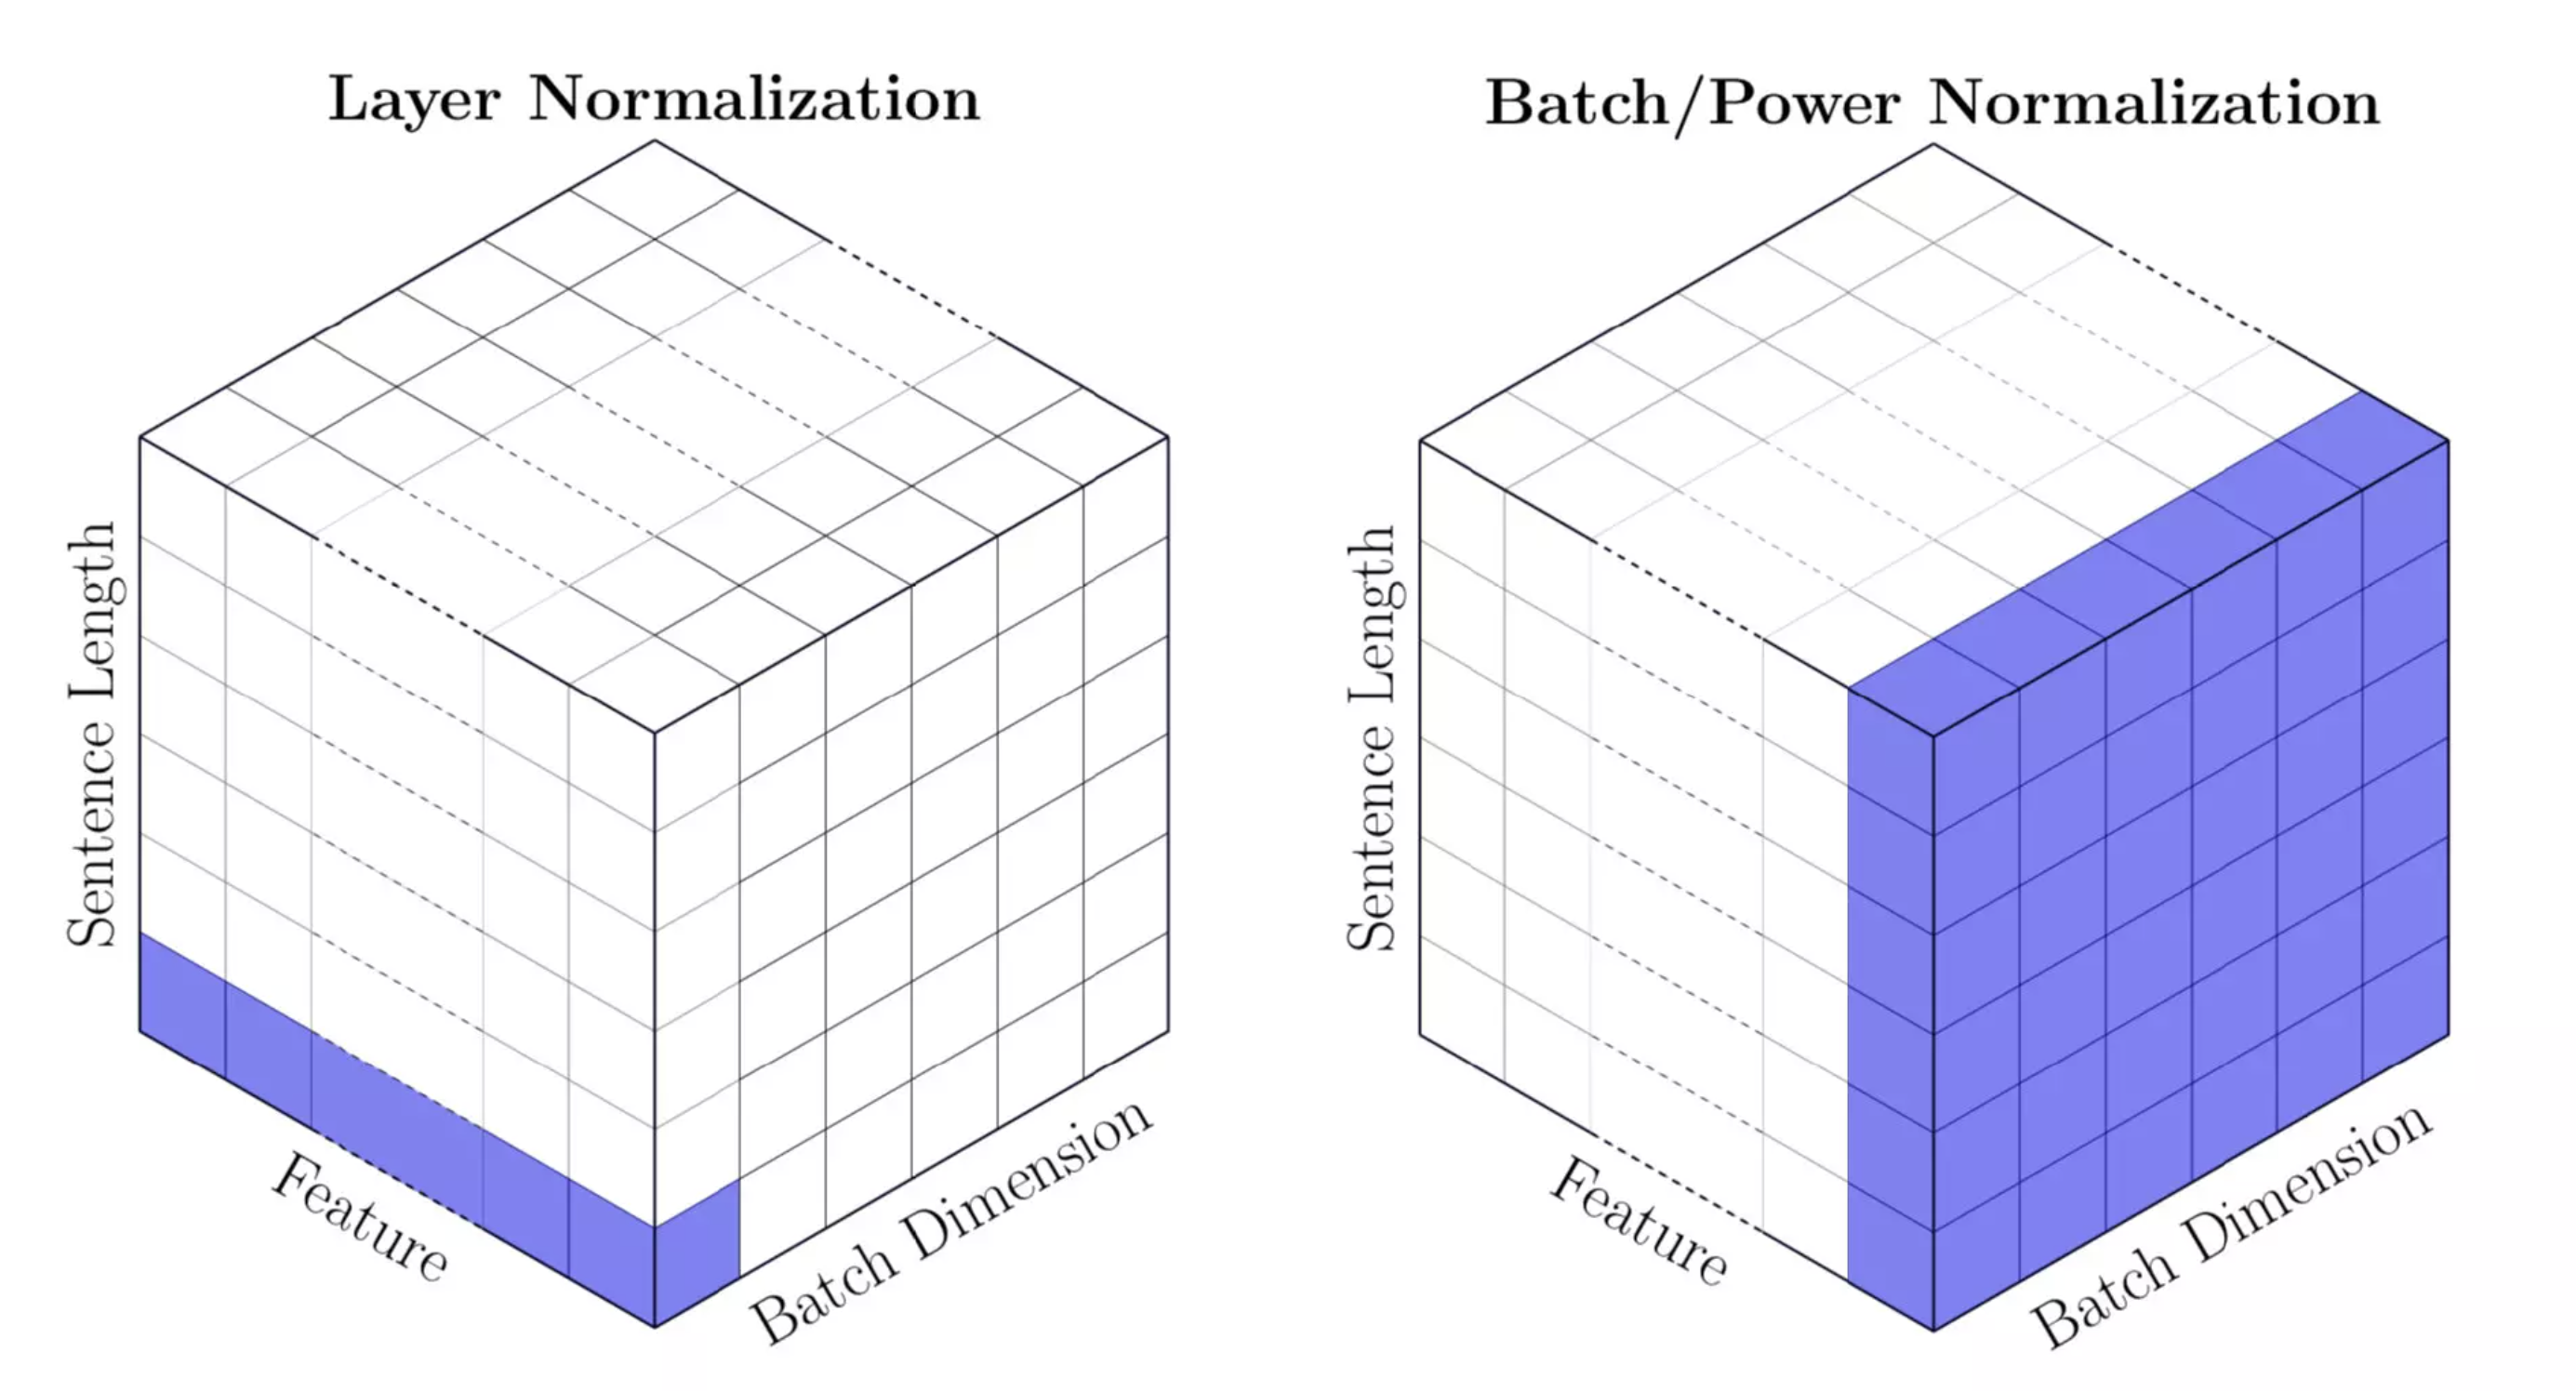
\includegraphics[width=.8\linewidth]{layer.png}
	\end{center}
\end{frame}


\begin{frame}{Две модели рядом} 
	\begin{center}
		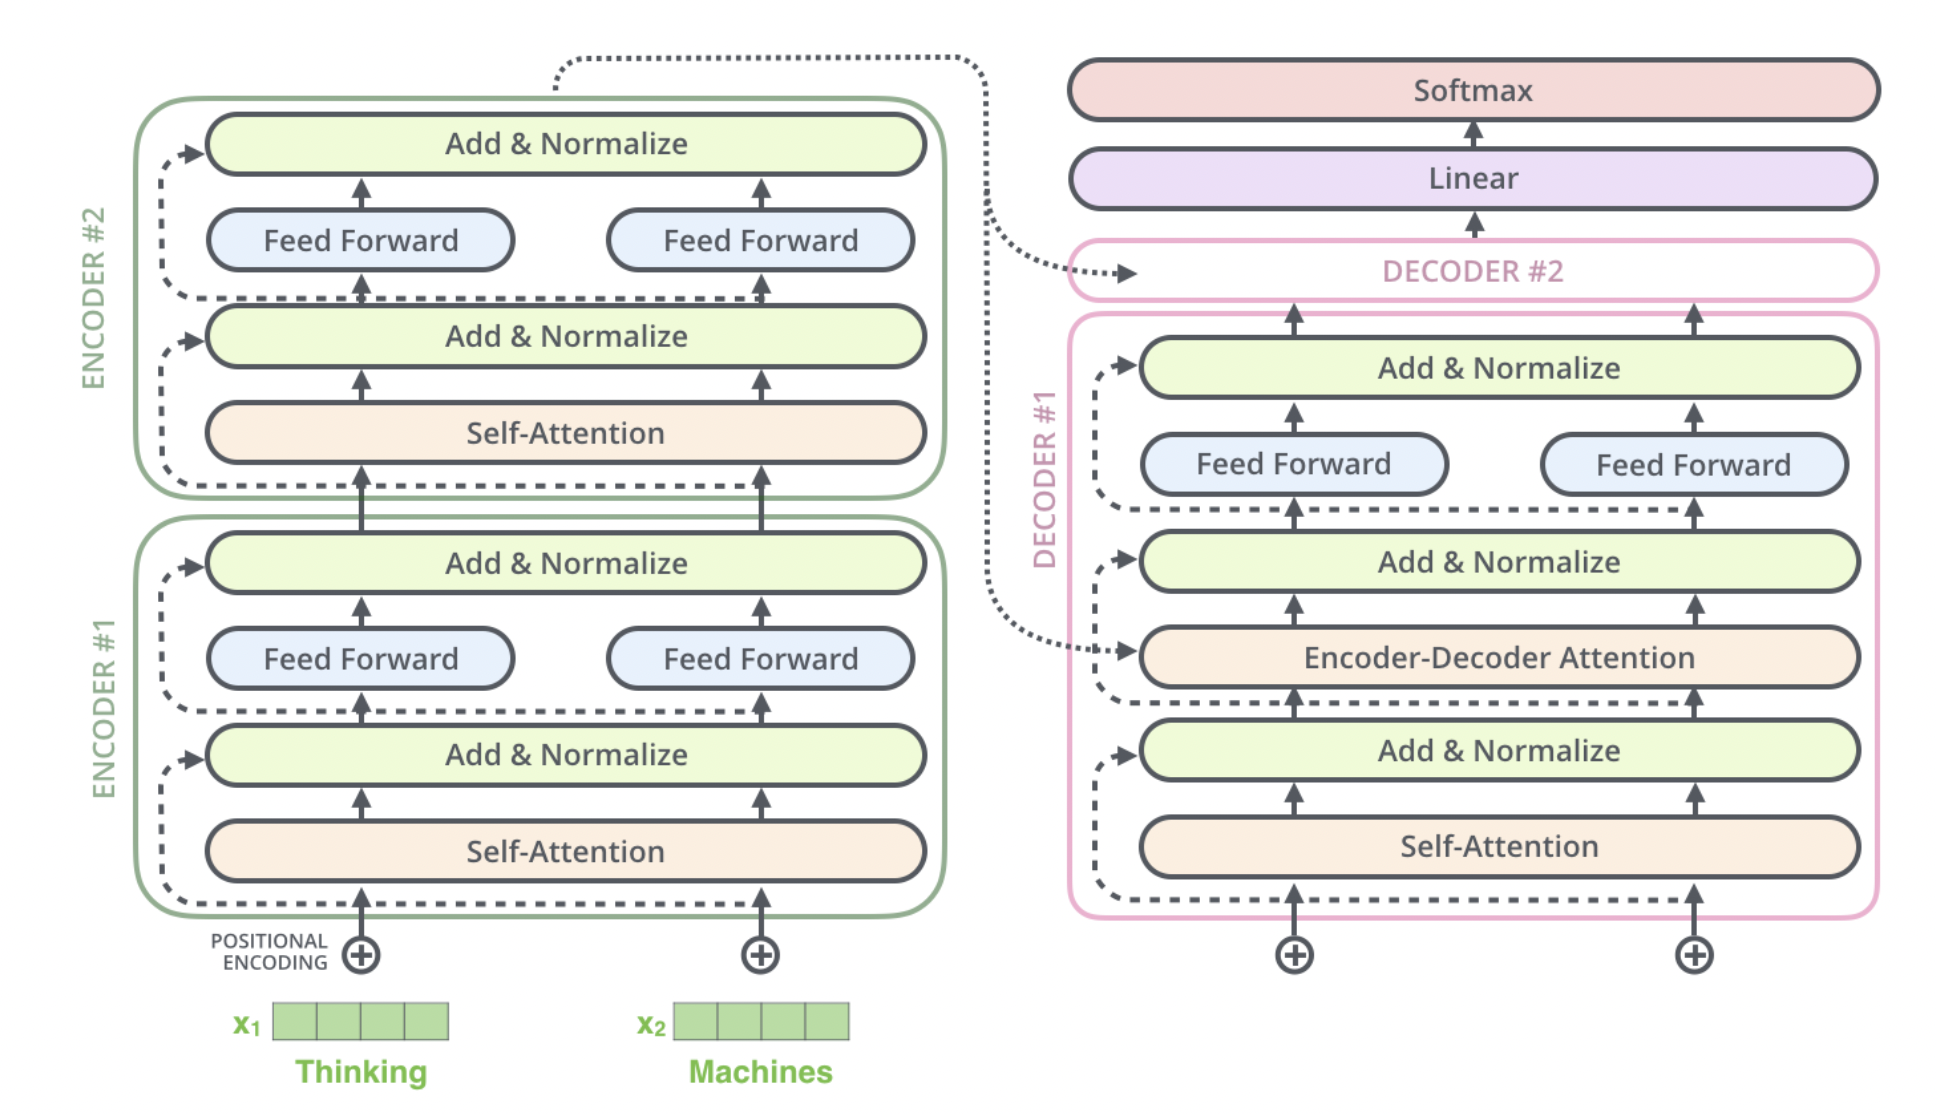
\includegraphics[width=.8\linewidth]{enc_dec.png}
	\end{center}
	\vfill
	\footnotesize
	{\color{blue} \url{http://jalammar.github.io/illustrated-transformer/}}
\end{frame}



\begin{frame}{Что происходит в декодере?} 
	\begin{center}
		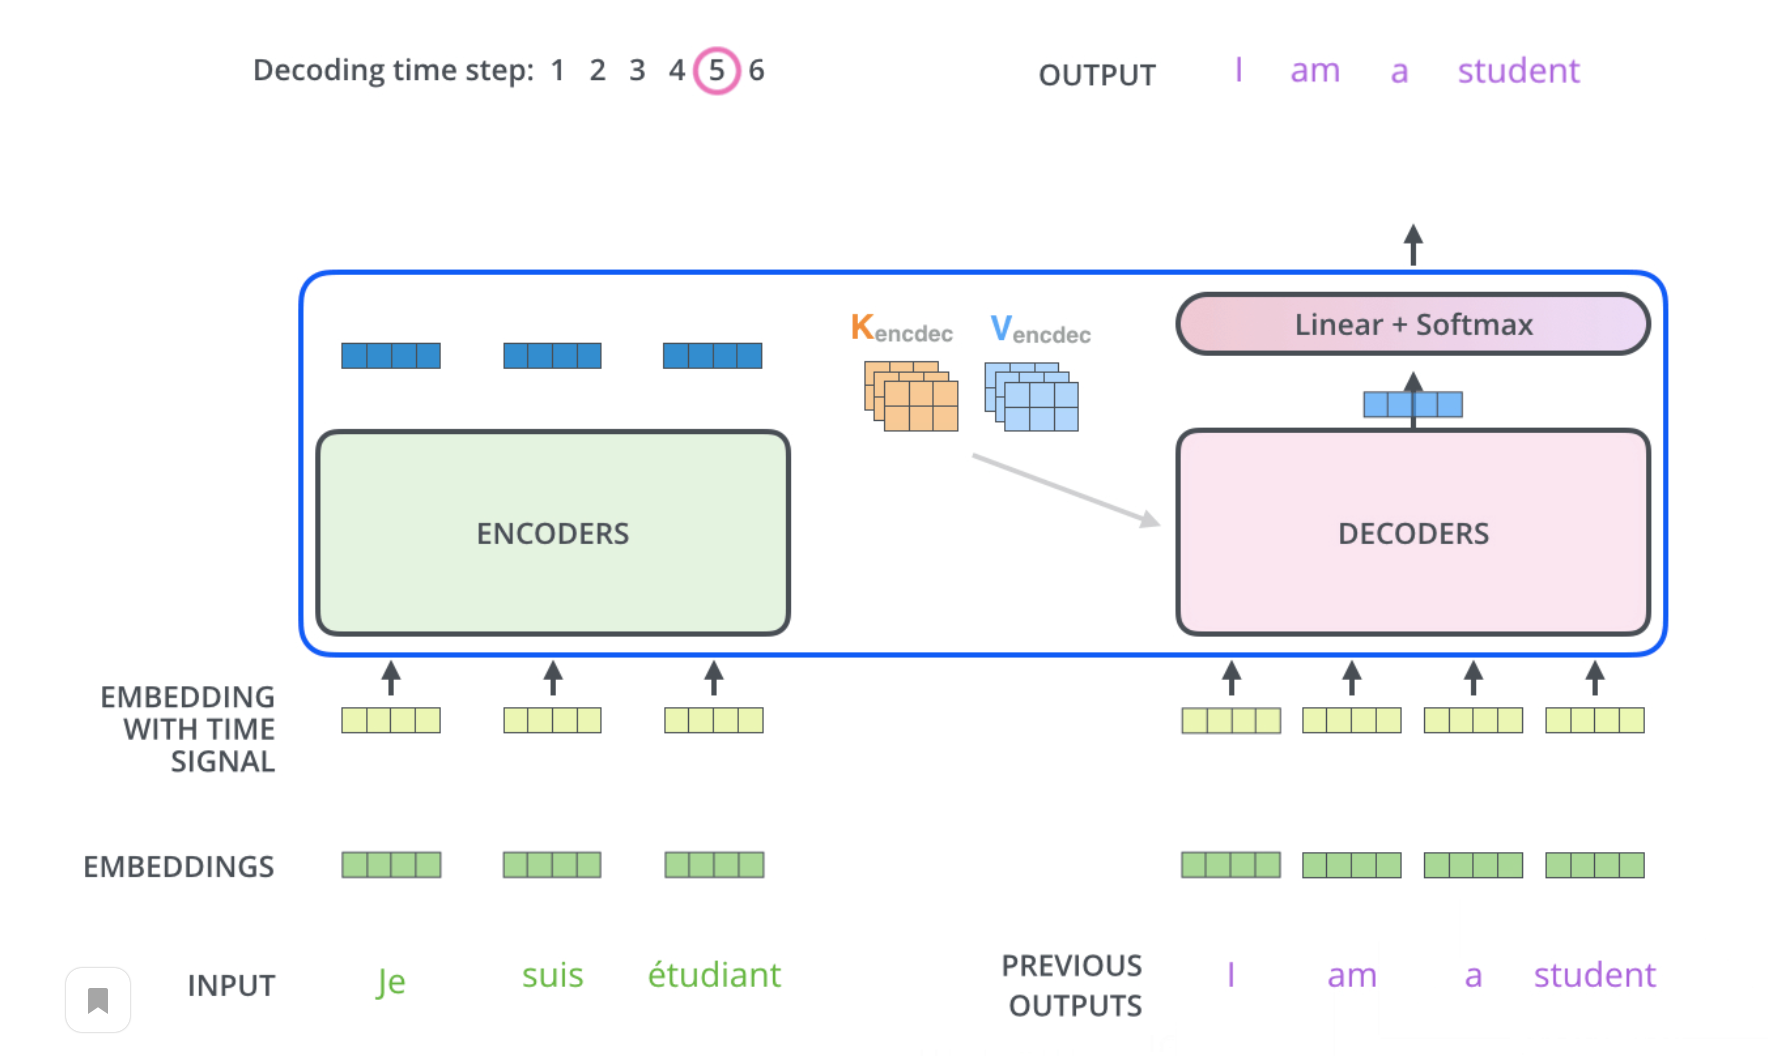
\includegraphics[width=.8\linewidth]{decoder.png}
	\end{center}
	\vfill
	\footnotesize
	{\color{blue} \url{http://jalammar.github.io/illustrated-transformer/}}
\end{frame}


\begin{frame}{Encoder-Encoder attention}
	\begin{center}
		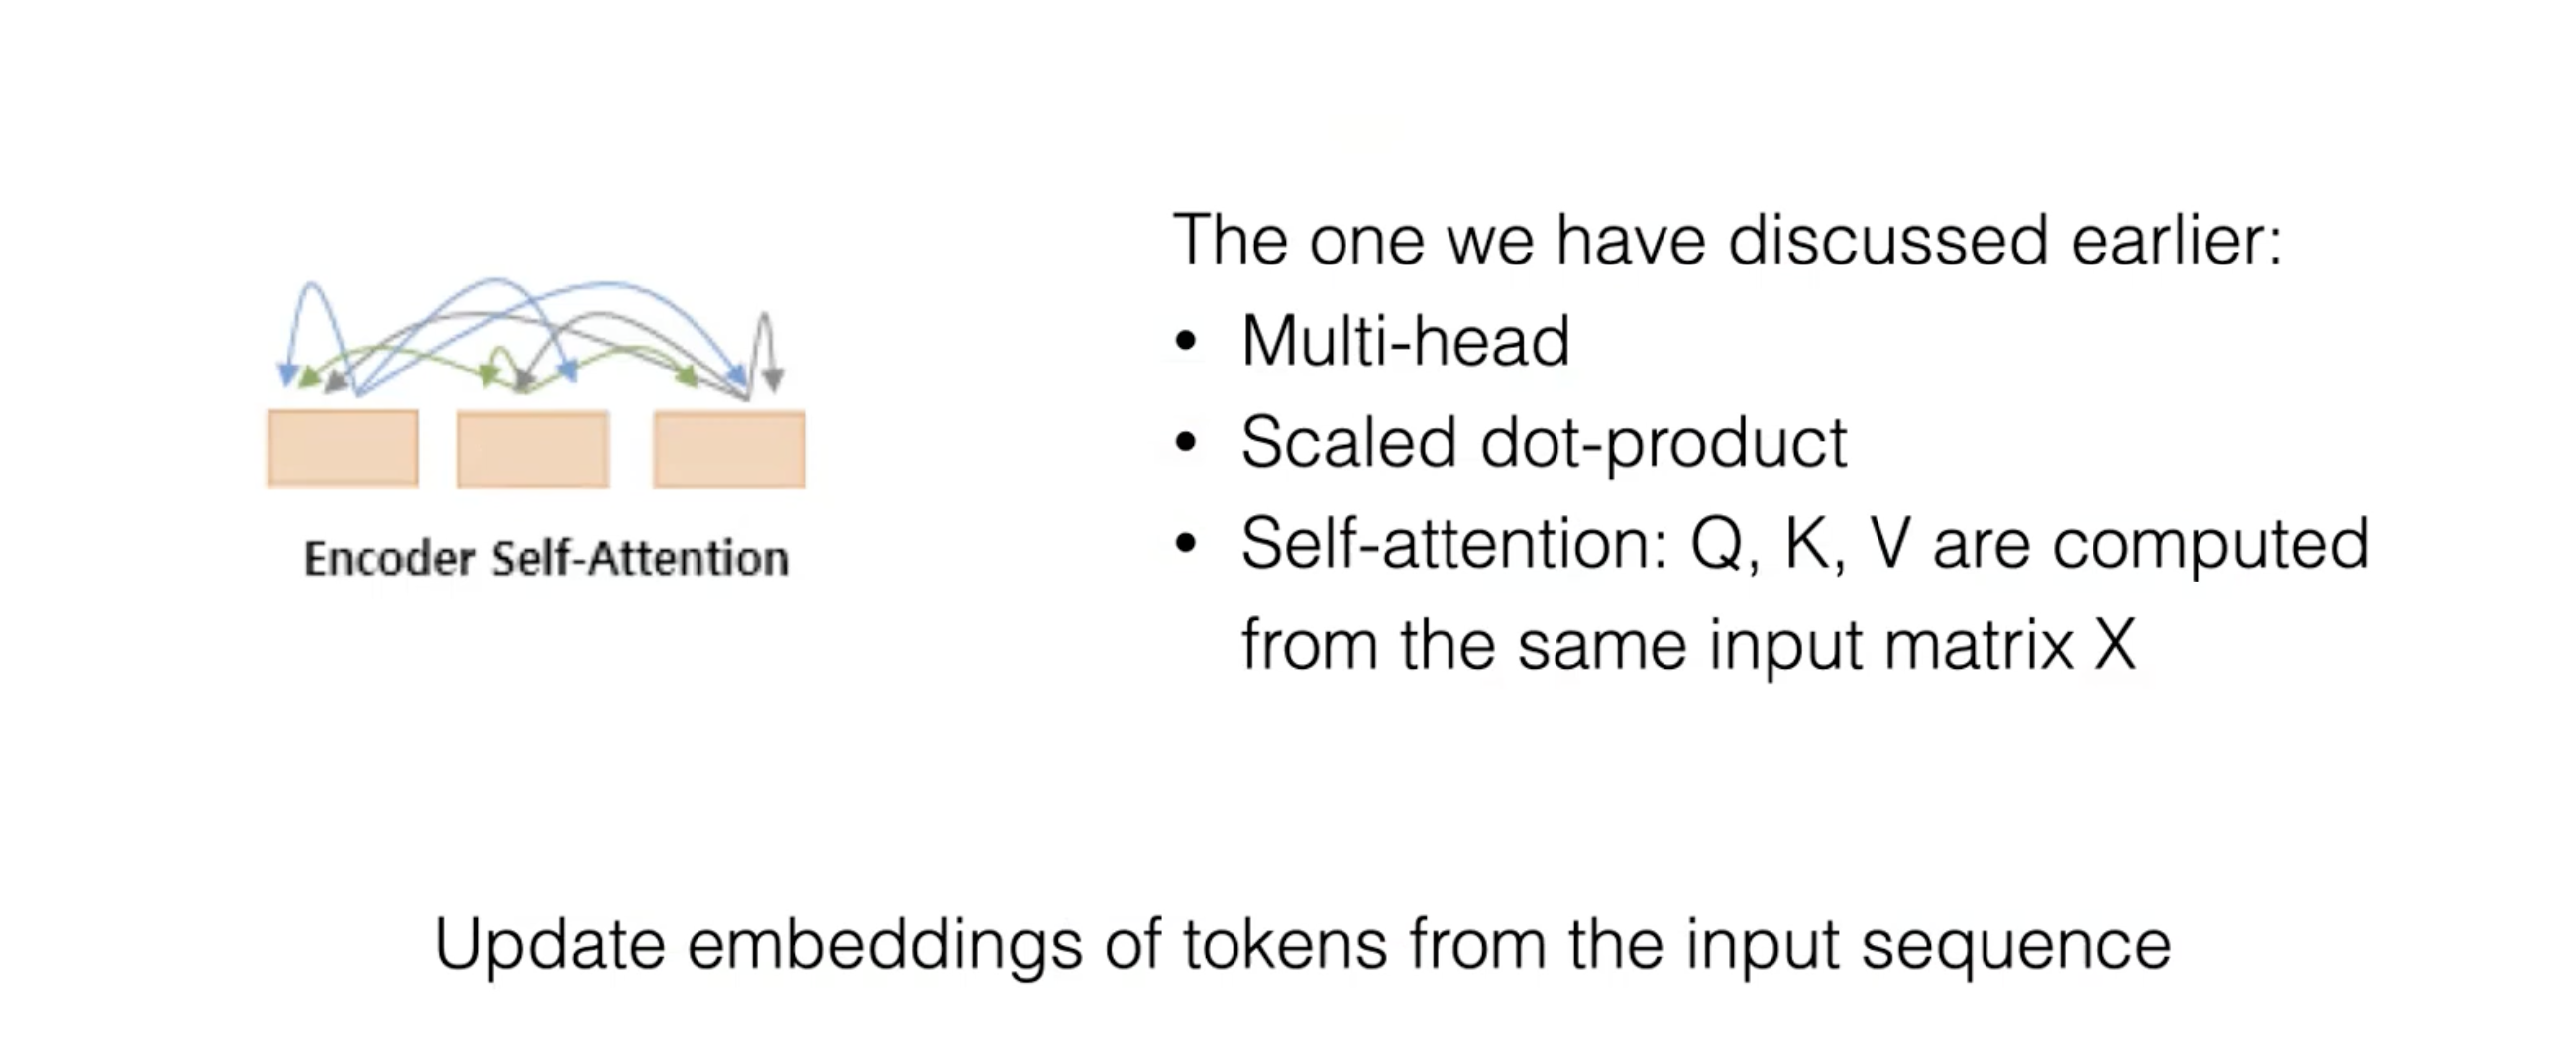
\includegraphics[width=.99\linewidth]{enc_enc_att.png}
	\end{center}
\end{frame}


\begin{frame}{Decoder-Decoder attention}
	\begin{center}
		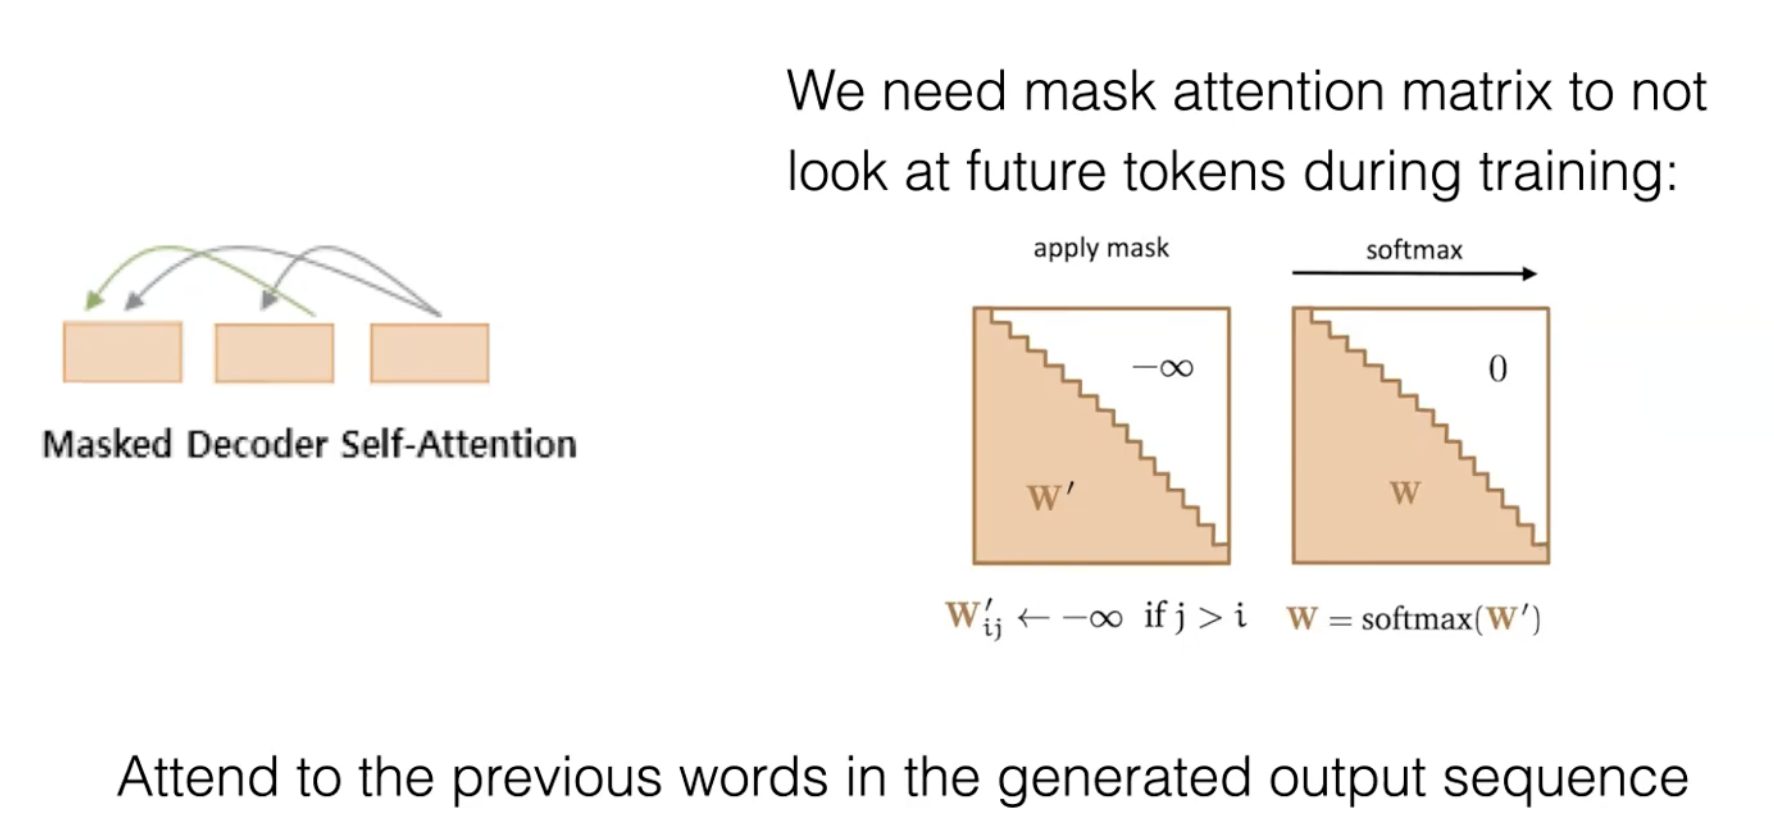
\includegraphics[width=.99\linewidth]{dec_dec_att.png}
	\end{center}
\end{frame}


\begin{frame}{Encoder-Decoder attention}
	\begin{center}
		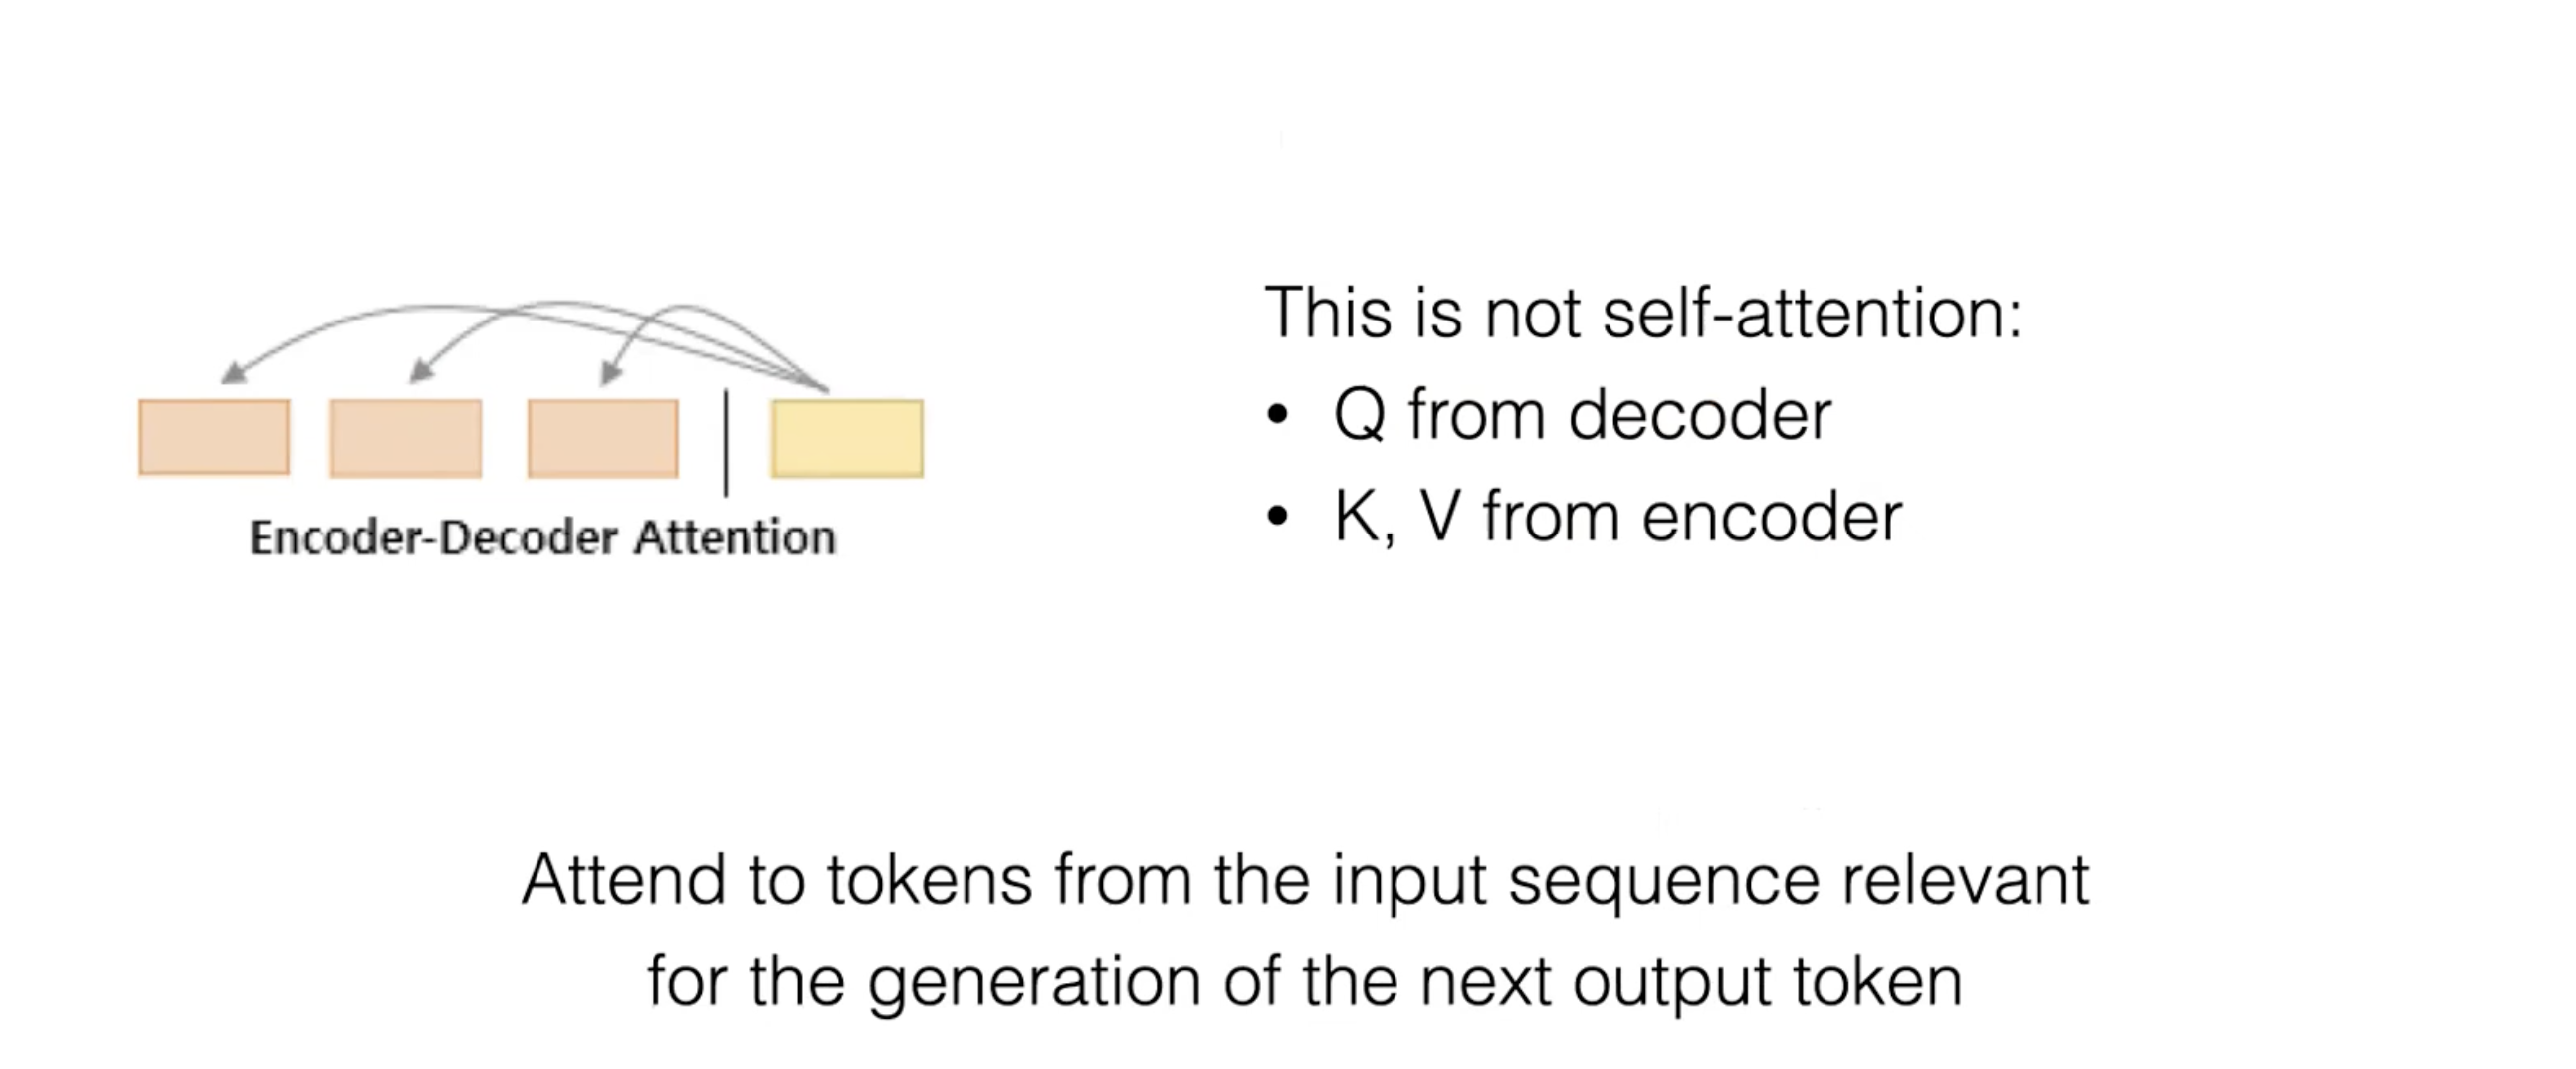
\includegraphics[width=.99\linewidth]{enc_dec_att.png}
	\end{center}
\end{frame}


\begin{transitionframe}
	\begin{center}
		\Huge Обучение 
	\end{center}
\end{transitionframe}

\begin{frame}{Trainig details}
	\begin{center}
		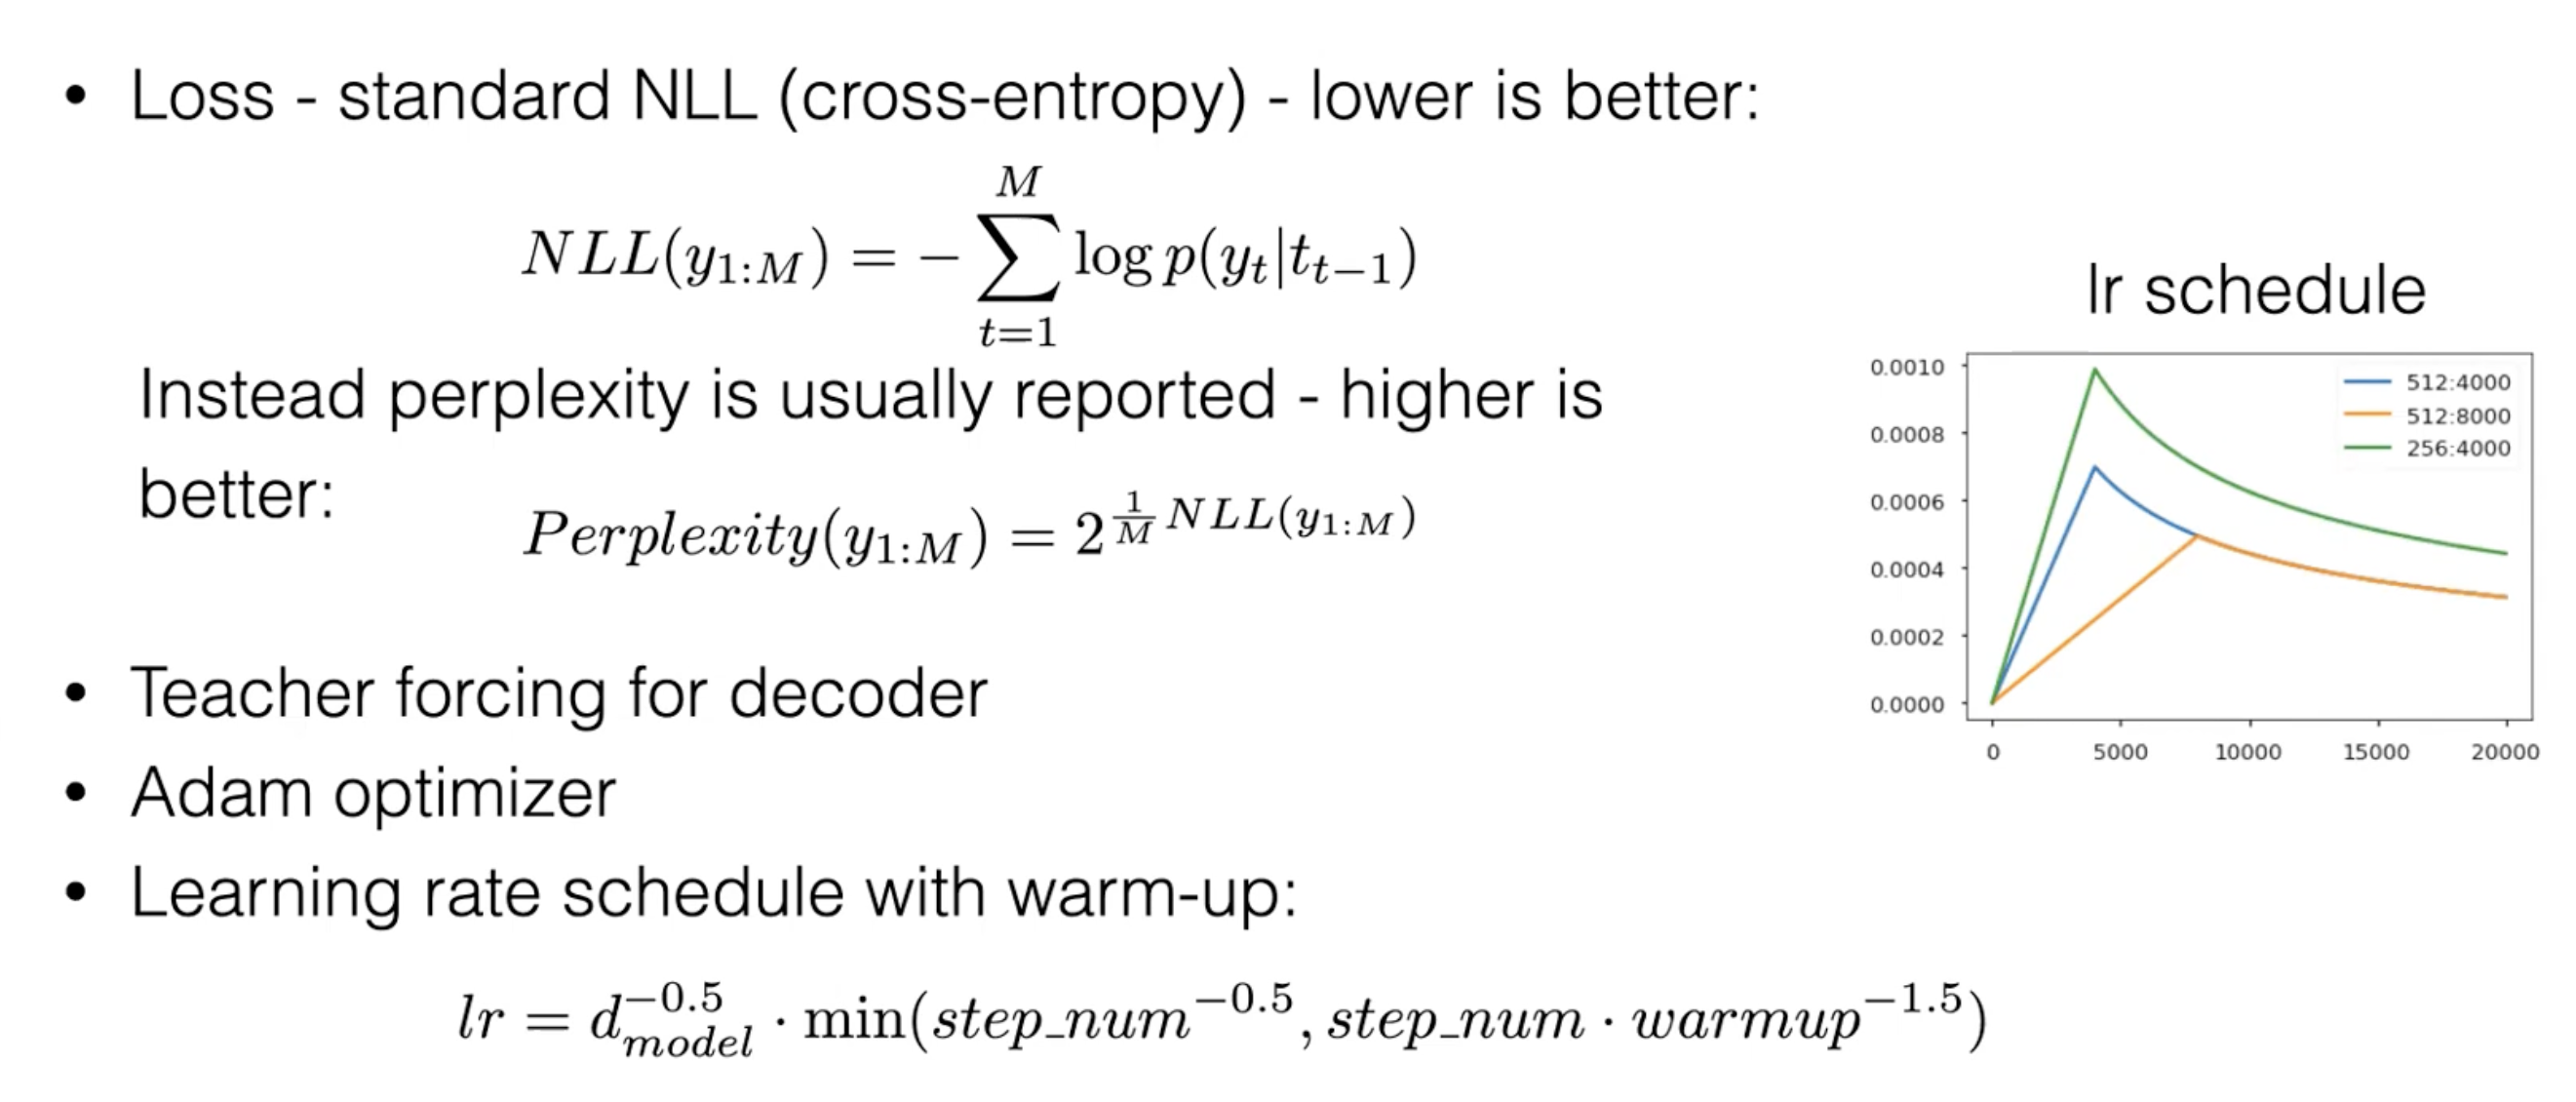
\includegraphics[width=.99\linewidth]{train01.png}
	\end{center}
\end{frame}


\begin{frame}{Trainig details}
	\begin{center}
		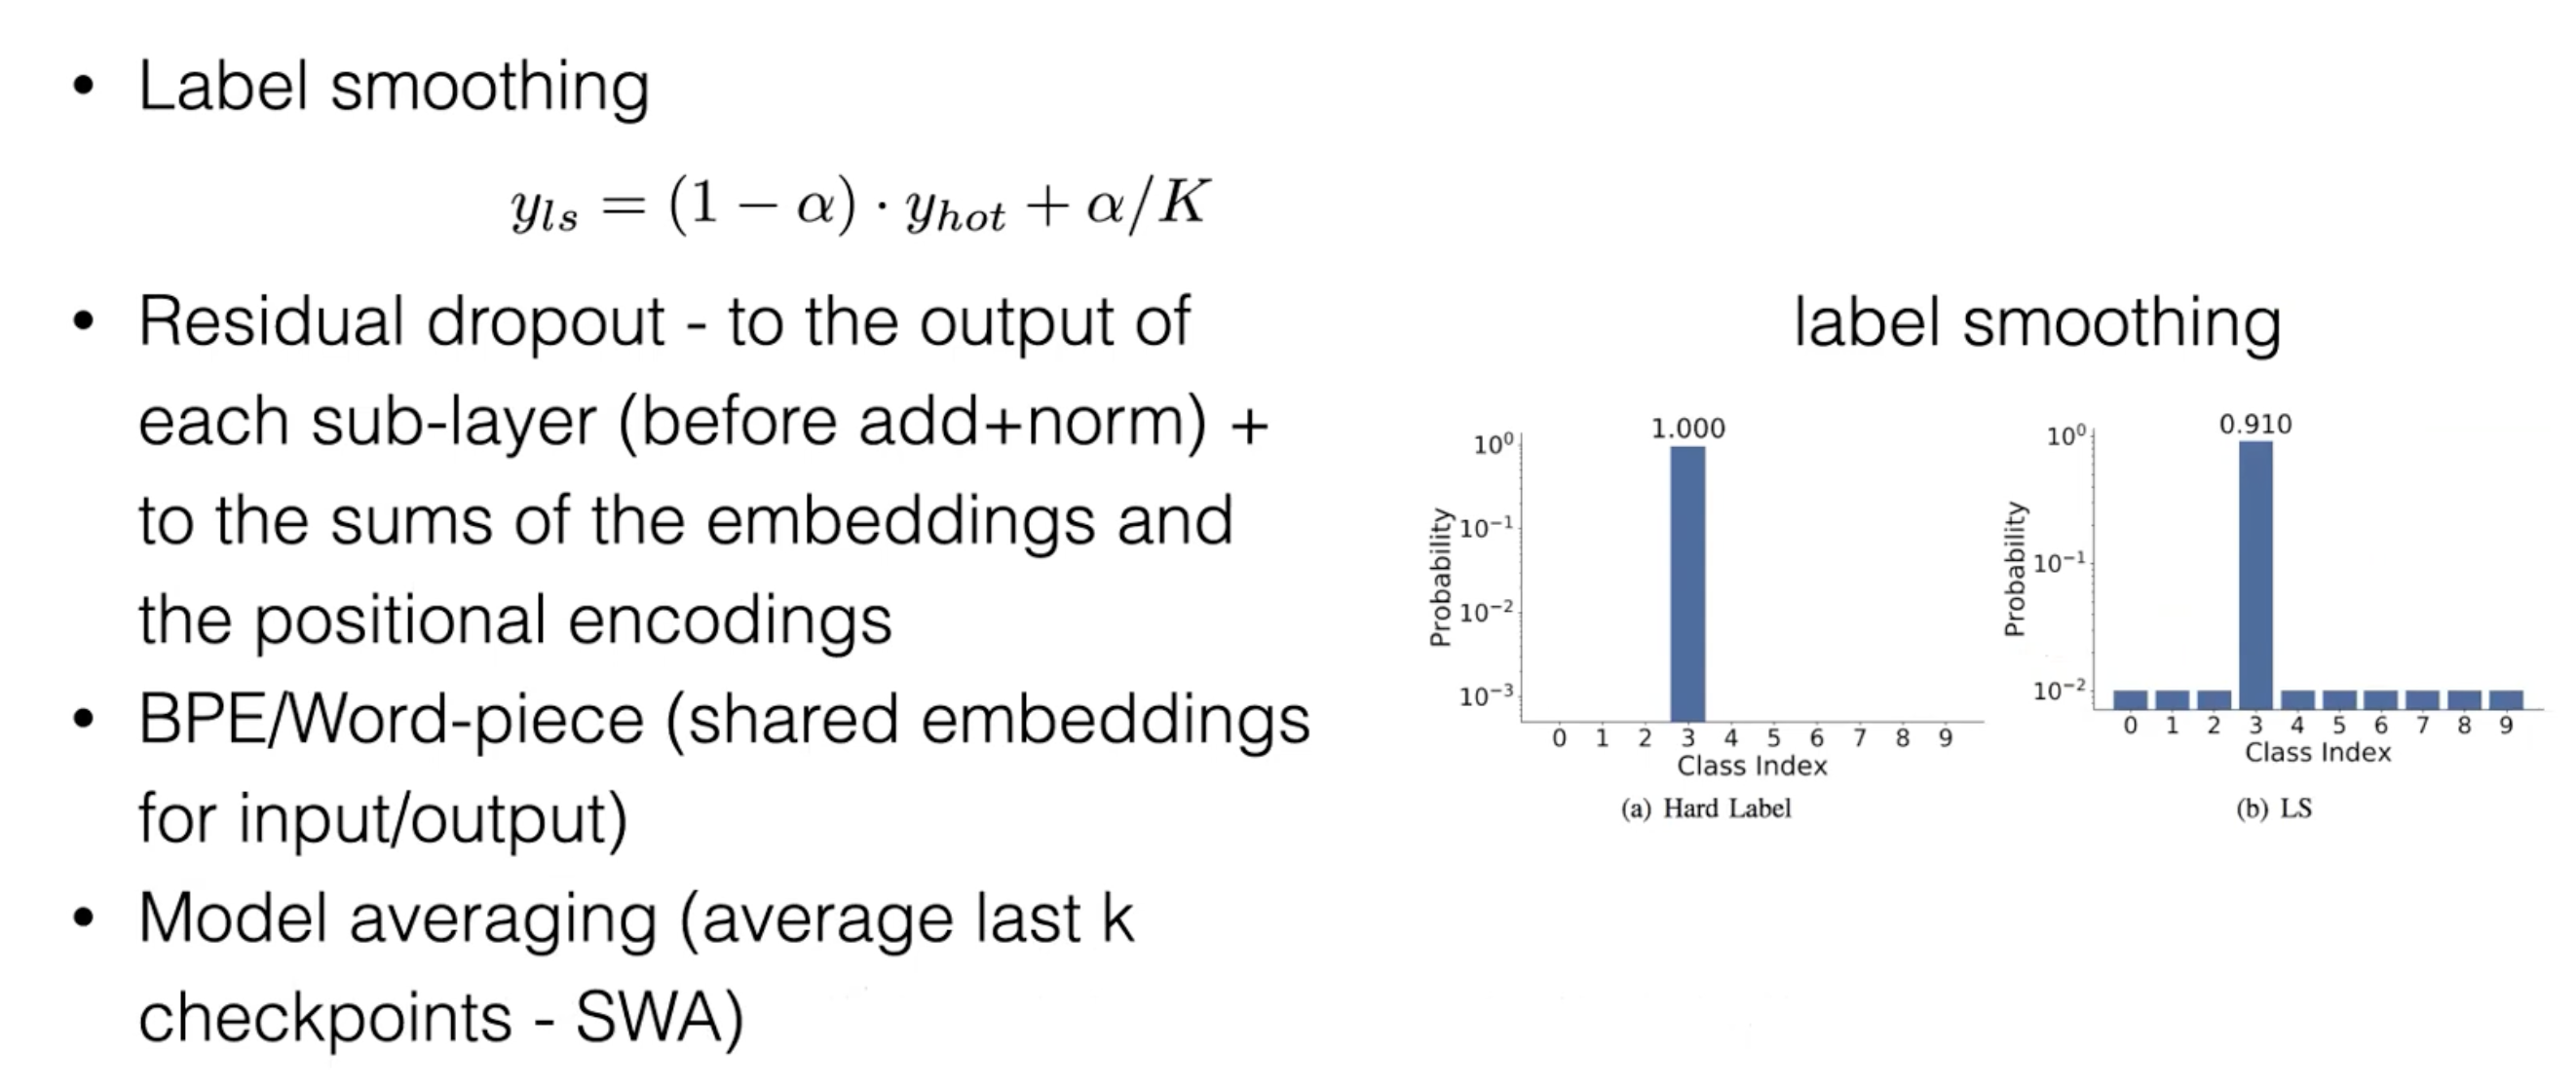
\includegraphics[width=.99\linewidth]{train02.png}
	\end{center}
\end{frame}



\begin{transitionframe}
	\begin{center}
		\Huge Contextualized Word Embeddings
	\end{center}
\end{transitionframe}

\begin{frame}{Embeddings in NPL} 
	\begin{wideitemize}
		\item  Большие объёмы неразмеченных данных в интернете в разных доменах (книги,
		новости, википедия, иные тексты из интернет-страниц)
		\item  Размеченных данных мало. Качественная разметка дорогая и долгая
		\item  Много вычислительных ресурсов, GPU, TPU, фреймворки распределённх
		вычислений
		\item Можем ли мы как-то заиспользовать имеющиеся ресурсы?
	\end{wideitemize}
\end{frame}

\begin{frame}{Individual embeddings }
	\begin{center}
			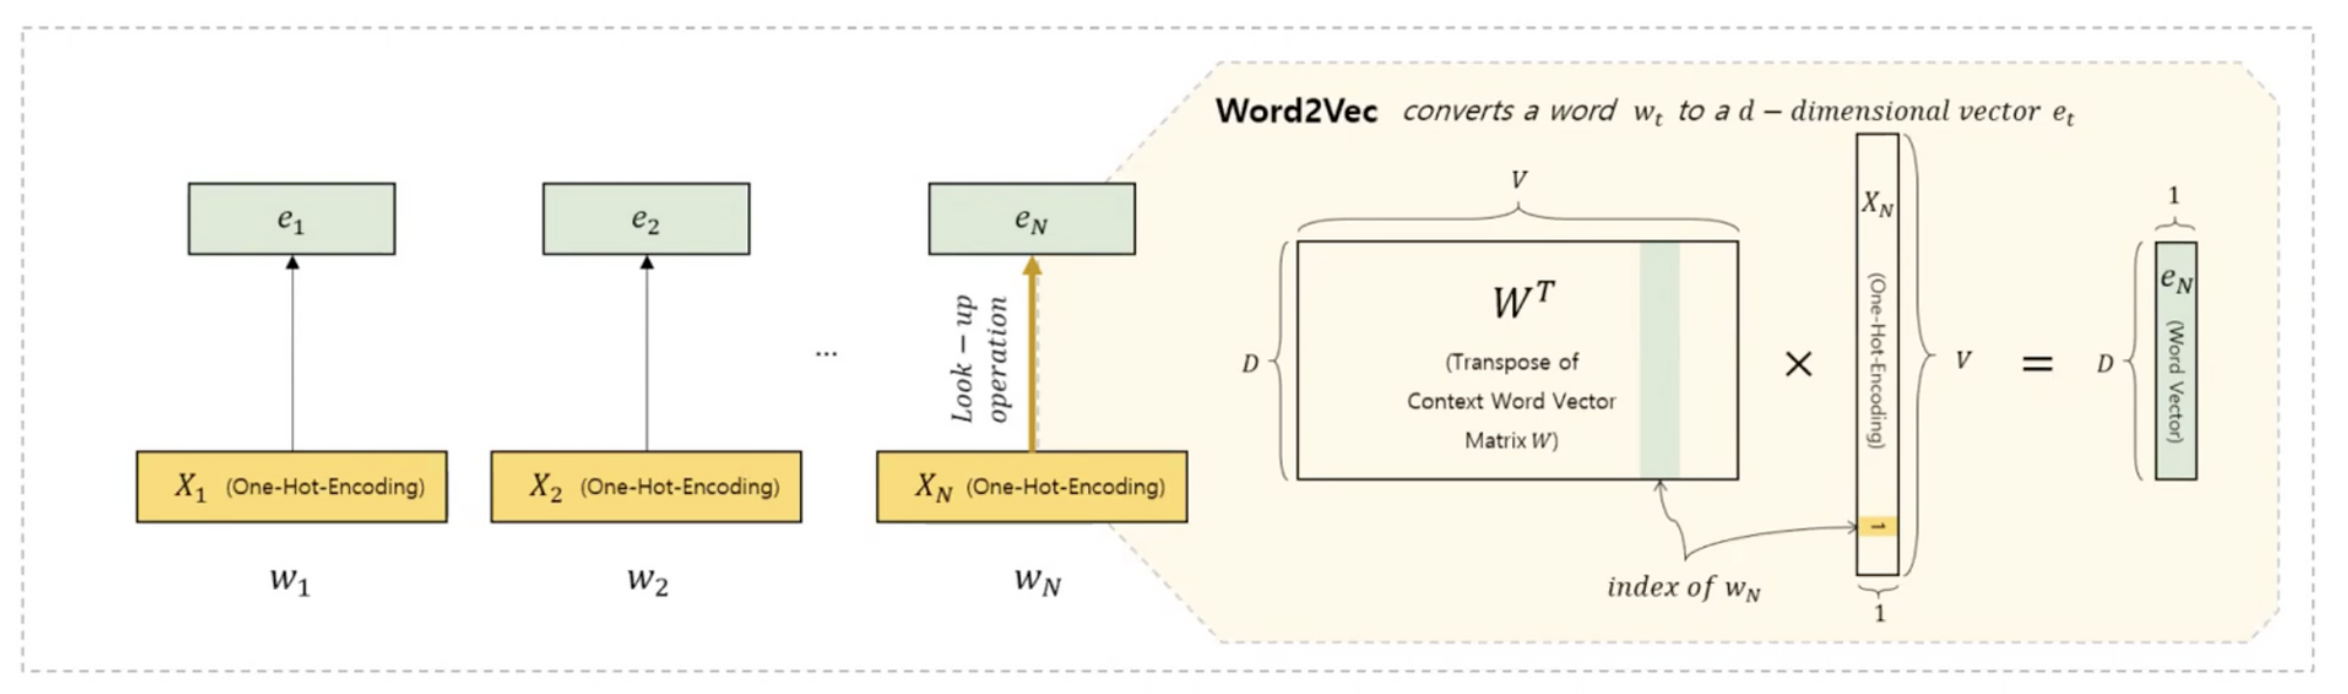
\includegraphics[width=.99\linewidth]{ind_emb.png}
	\end{center}

	\alert{word2vec, GLOVE, fasttext \ldots} 
\end{frame}

\begin{frame}{Contextualised embeddings}
	\begin{wideitemize}
		\item Обучаем большую модель трансформер на какой-нибудь unsupervised задаче на очень больших данных (очень долго, порядка нескольких недель);
		\item Дообучаем модель на конкретную задачку на малом корпусе размеченных данных (очень быстро, порядка 1 часа на одной ГПУ).
	\end{wideitemize}
\end{frame}

\begin{frame}{Contextualised embeddings}
	\begin{center}
		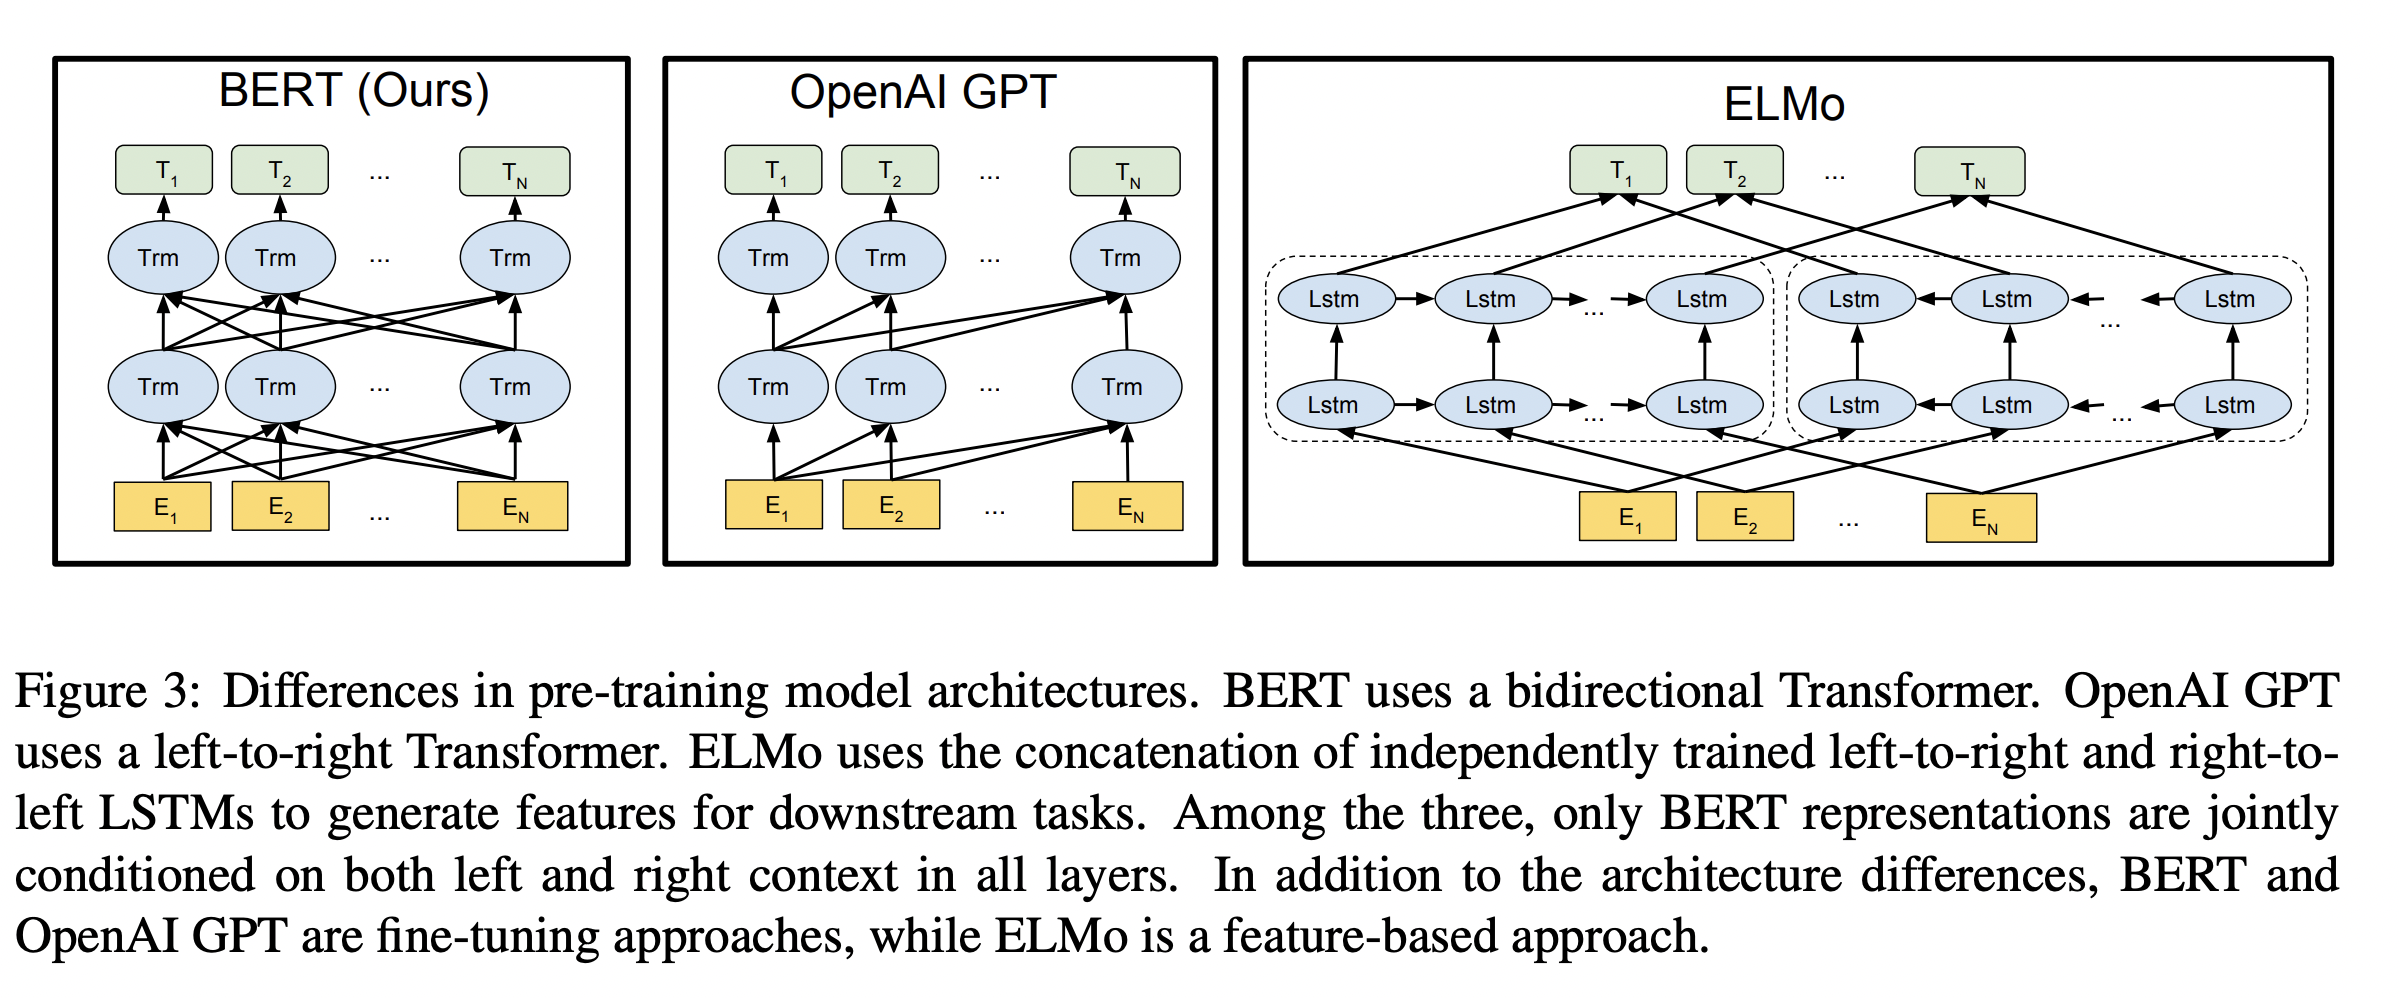
\includegraphics[width=.99\linewidth]{bert.png}
	\end{center}
	\vfill
	\footnotesize
	{\color{blue} \url{https://arxiv.org/pdf/1810.04805.pdf}}
\end{frame}


\begin{frame}{ Embeddings from Language Models (ELMo)}
	\begin{center}
		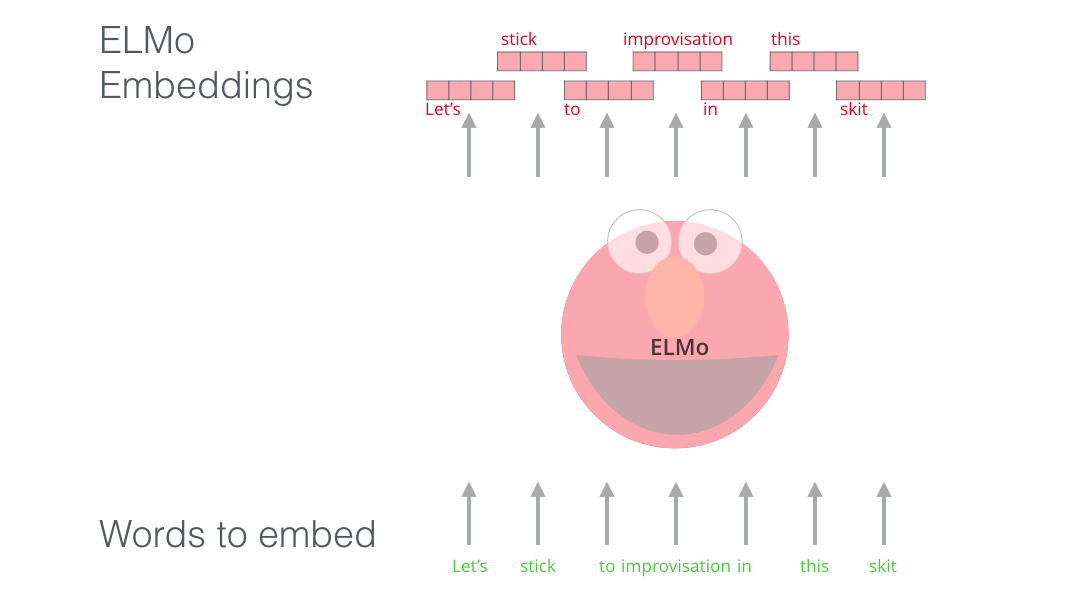
\includegraphics[width=.8\linewidth]{elmo1.png}
	\end{center}
	\vfill
	\footnotesize
	{\color{blue} \url{https://jalammar.github.io/illustrated-bert/}  } 
\end{frame}


\begin{frame}{ Embeddings from Language Models (ELMo)}
	\begin{center}
		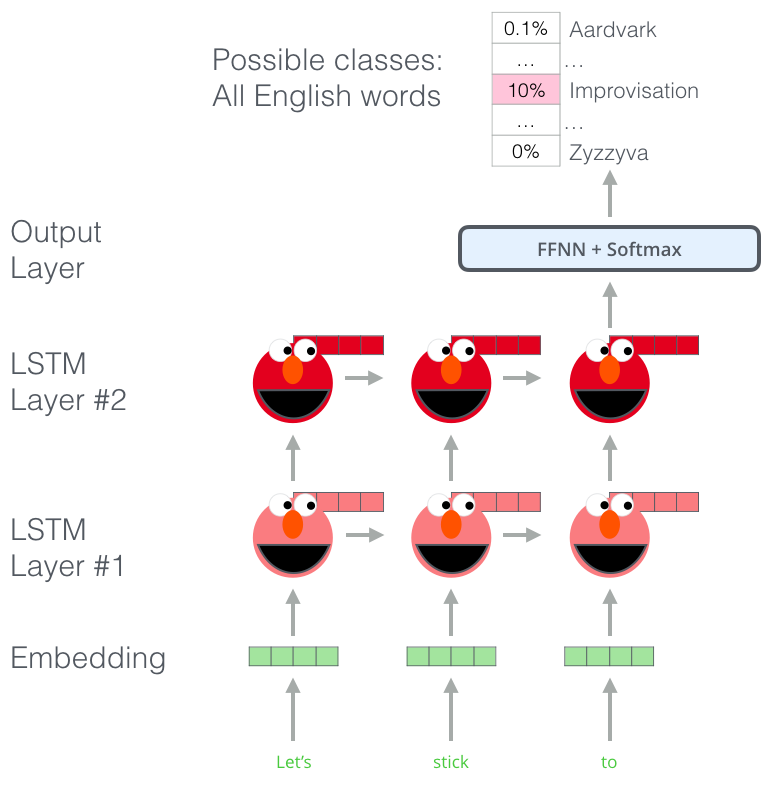
\includegraphics[width=.5\linewidth]{elmo2.png}
	\end{center}
\end{frame}

\begin{frame}{ Embeddings from Language Models (ELMo)}
	\begin{center}
		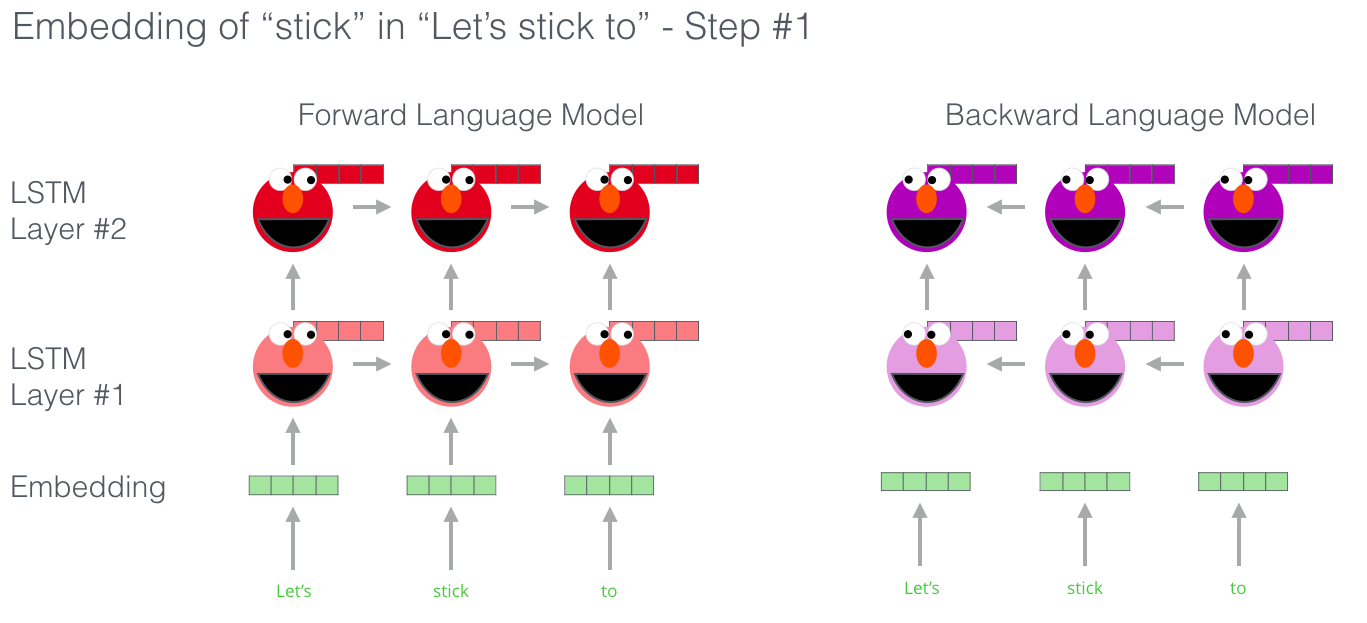
\includegraphics[width=.9\linewidth]{elmo3.png}
	\end{center}
\end{frame}

\begin{frame}{ Embeddings from Language Models (ELMo)}
	\begin{center}
		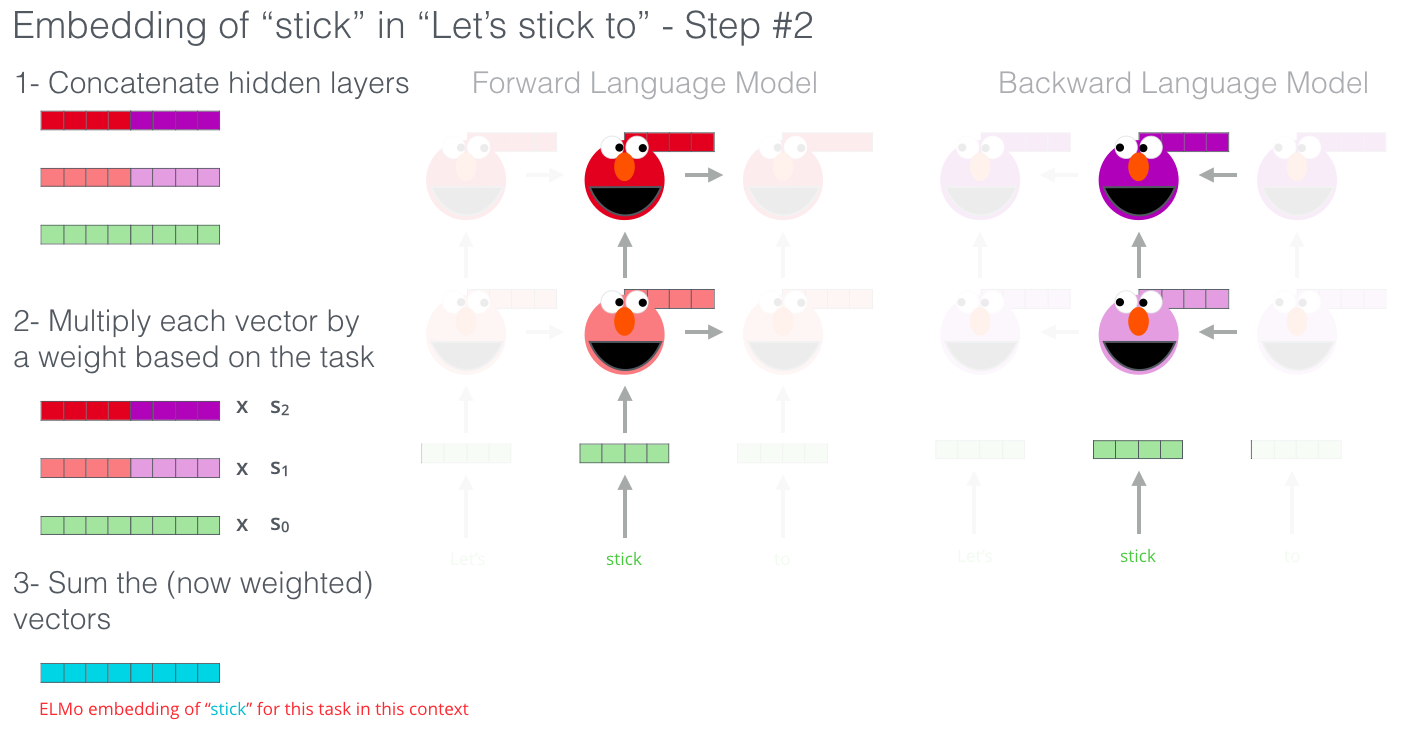
\includegraphics[width=.9\linewidth]{elmo4.png}
	\end{center}
\end{frame}


\begin{frame}{ Embeddings from Language Models (ELMo)}
	\begin{center}
		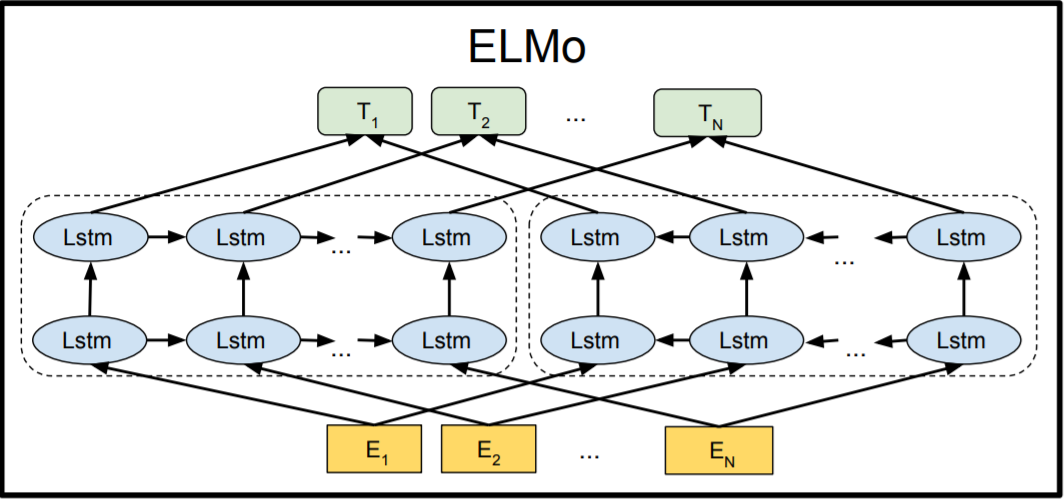
\includegraphics[width=.6\linewidth]{ elmo.png}
	\end{center}
	В качестве эмбеддинга используется вектор $[𝑇 , h_𝑙, h_𝑟]$, где $𝑇$ - токены, которые сетка выплёвывает наружу, $h_𝑙$ - итоговое скрытое состояние ячеек при проходе слева направо, $h_𝑟$ - справа налево.
	\vfill
	\footnotesize
	{\color{blue} \url{https://arxiv.org/pdf/1802.05365.pdf}  } 
\end{frame}


\begin{frame}{Особенности ELMO}
	\begin{wideitemize}
		\item  Учитывает порядок слов в тексте
		\item  Можно сгенерировать эмбеддинг для любой последовательности из токенов
		\item  Рекуррентные слои работают очень долго, хочется быстрее
	\end{wideitemize}
\end{frame}


\begin{frame}{BERT (2018)}
	\begin{wideitemize}
		\item  \alert{Bidirectional Encoder Representations from Transformers} 
		\item Предобученный на искутсвенно придуманной задаче  энкодер
		\item Его можно файн-тьюнить для решения других задач 
	\end{wideitemize}
\end{frame}


\begin{frame}{BERT (2018)}
	\begin{center}
		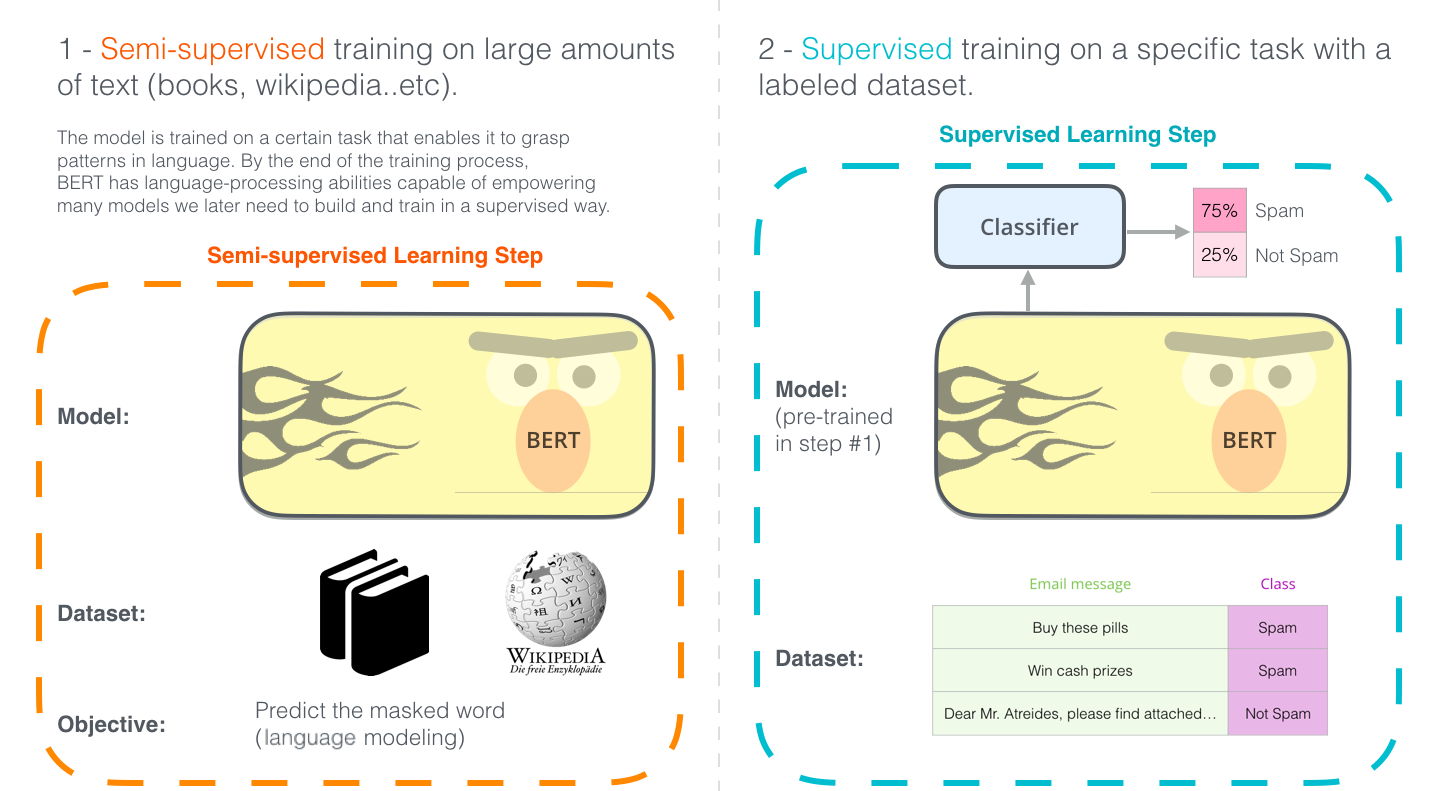
\includegraphics[width=0.8\linewidth]{BERT_stud}
	\end{center}
	\vfill
	\footnotesize
	{\color{blue} \url{http://jalammar.github.io/illustrated-bert/}}
\end{frame}


\begin{frame}{BERT}
	\begin{wideitemize}
		\item  \alert{Masked Language Model: }  выкидываем часть слов (обычно $15\%$), модель должна их восстановить:
				\begin{itemize}
					\item $80\%$ меняем на токен <MASK>
					\item $10\%$ меняем на случайные
					\item $10\%$ не меняем			
				\end{itemize}
		
		Мы предсказываем пропуски, считаем Loss по всем $15\%$. Случайные и неизменные токены позволяют не переобучиться под токен <MASK>.
				
		\item  \alert{Next Sentence Prediction:}  подаём на вход два предложения, модель должна понять в каком порядке они идут. Правда ли второе является продолжением первого. Эта задача помогает модели понять концепцию предложения.
	\end{wideitemize}
\end{frame}


\begin{frame}{CLS-токен}
	Пример токенезированного предложения:
	\begin{center}
		\alert{[CLS]} my dog is cute \alert{[SEP]} he likes play \#\#ing \alert{[SEP]}
	\end{center}

	\only<1>{
		\begin{wideitemize}
			\item \alert{[CLS]} — специальный токен, который мы добавляем к началу любого предложения, он несет информацию о всей входной последовательности (а вход состоит из двух предложений)
			
			\item  \alert{[SEP]} — специальный токен, который говорит, что слева от него первое предложение, а справа — второе
			
			\item  \alert{\#\#} — специальный токен, обозначающий, что это кусок слова
		\end{wideitemize}
	}

	\only<2>{

			\vspace{0.3cm}
			Мы токенезируем предложение, для каждого токена учим эмбеддинг. Поскольку у нас трансформер, мы добавляем к эмбеддингам слов позиционный эмбеддинг и дополнительно добавляем эмбеддинг, отвечающий за то, в каком из двух предложений мы находимся. Все три эмбеддинга суммируются.
			$$
				E = E_{word} + E_{pos} + E_{sent}
			$$

	}
\end{frame}







\begin{frame}{BERT}
		\begin{center}
			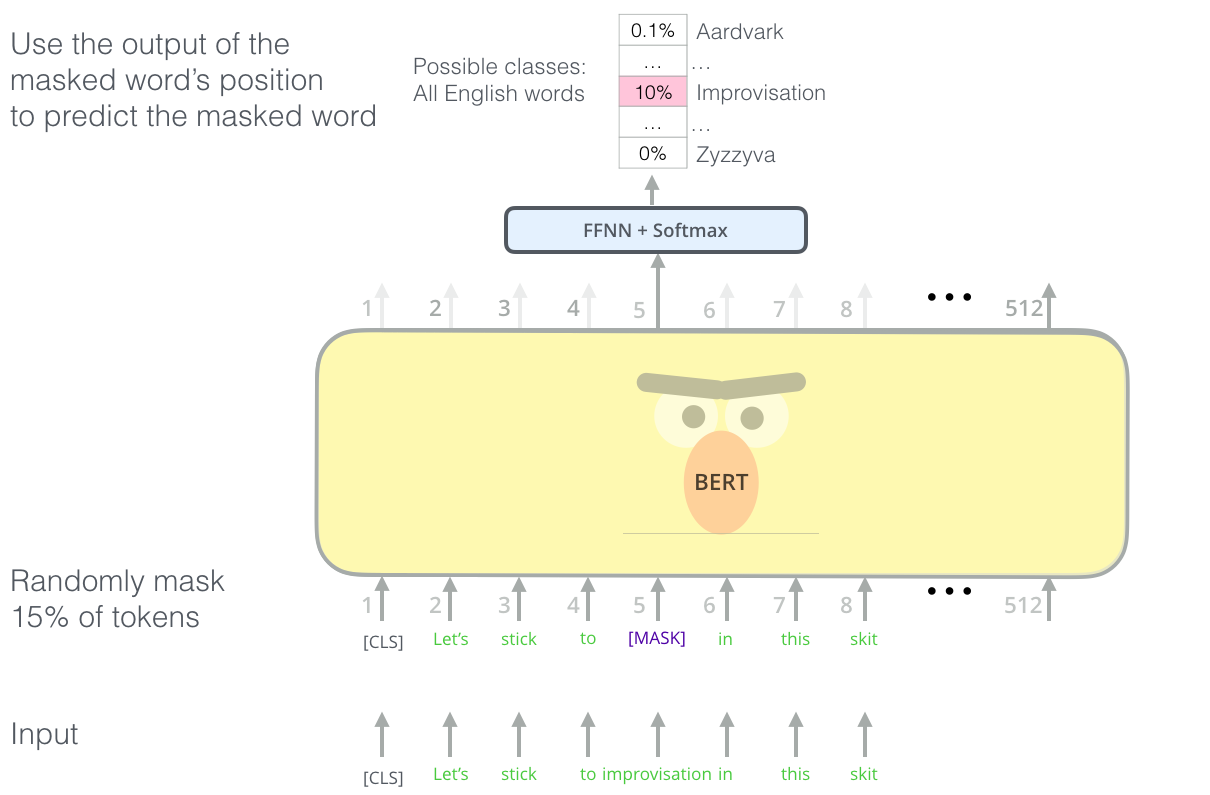
\includegraphics[width=0.7\linewidth]{pre_train_bert}
		\end{center}
		\vfill
		\footnotesize
		{\color{blue} \url{http://jalammar.github.io/illustrated-bert/}}
\end{frame}


\begin{frame}{BERT}
		\begin{center}
			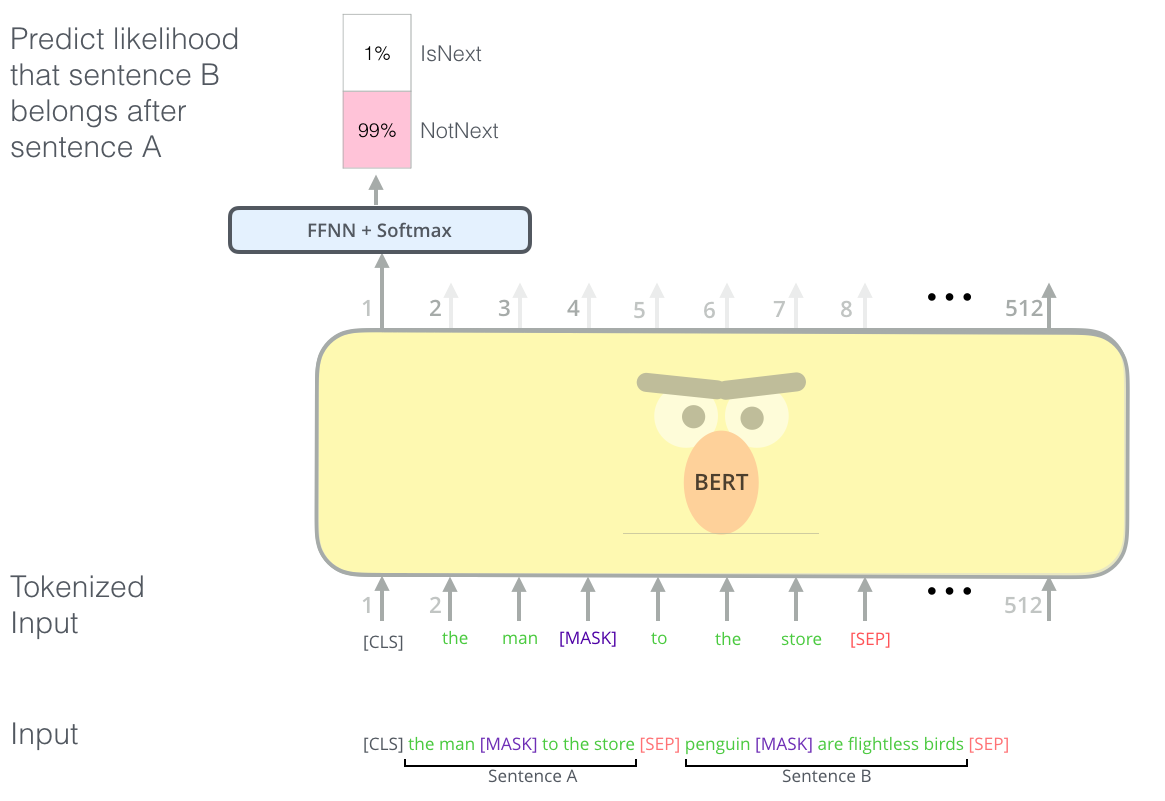
\includegraphics[width=0.65\linewidth]{bert_sent}
		\end{center}
		\vfill
		\footnotesize
		{\color{blue} \url{http://jalammar.github.io/illustrated-bert/}}
\end{frame}



\begin{frame}{Как применять (finetuning)}
	\begin{center}
		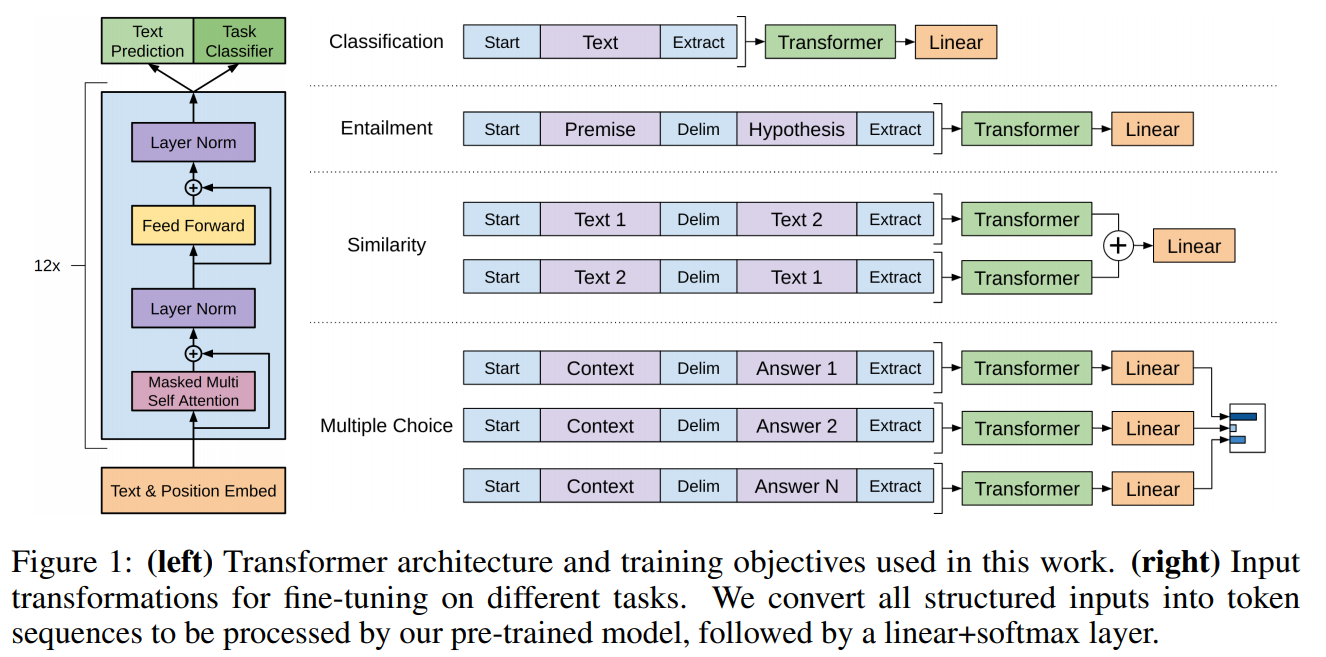
\includegraphics[width=0.9\linewidth]{images/use_models}
	\end{center}
\end{frame}


\begin{frame}{RoBERTa: A Robustly Optimized BERT (2019)}
	\alert{BERT был не дотюнен}

	\begin{wideitemize}
		\item  Взять больше данных, тренировать дольше
		\item Next sentence prediction лишний
		\item Более длинные предложения
		\item Большие батчи
		\item Динамическое маскирование
	\end{wideitemize}
	\vfill
	\footnotesize
	{\color{blue} \url{https://arxiv.org/abs/1907.11692}}
\end{frame}



\begin{frame}{GPT (Generative Pre-trained Transformer)}
	\begin{wideitemize}
		\item  Языковая модель на декодере трансформера
		\item  Умеет генерить продолжение текста. Настолько хорошо, что OpenAI
		отказался её публиковать и устроил мощный PR
		\item  Публикует понемногу, начиная с маленьких моделей
		\item  Разные языковые модели на трансформерах можно попробовать здесь: \url{
		https://transformer.huggingface.co/}
	\end{wideitemize}
\end{frame}


\begin{frame}{GPT}
	\begin{center}
	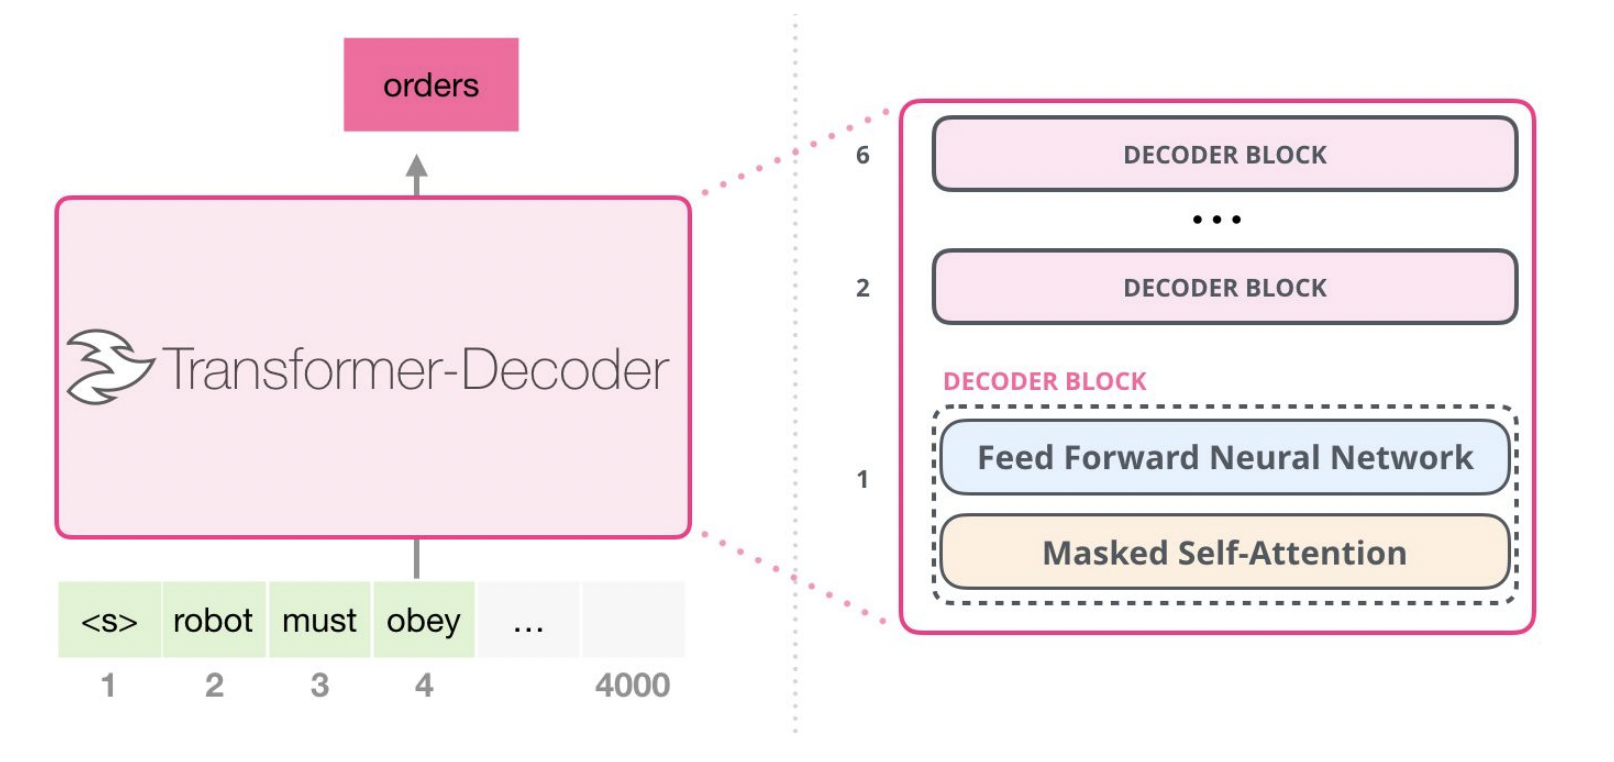
\includegraphics[width=0.9\linewidth]{masked_att_gpt.png}
\end{center}
	\vfill
	\footnotesize
	{\color{blue} \url{https://github.com/openai/gpt-2}}
\end{frame}



\begin{frame}{Language Model Zoo}
	\begin{center}
		
\includegraphics[width=.99\linewidth]{lang_zoo.png}
	\end{center}
	\vfill
	\footnotesize
	{\color{blue} \url{https://arxiv.org/pdf/1810.04805.pdf}}
\end{frame}

\end{document}
